\section{Architettura di sistema}
\subsection{Architettura di implementazione}
Il \textit{sistema}\textsubscript{\textit{G}} richiede la capacità di elaborare dati provenienti da diverse fonti in tempo reale e di fornire una visualizzazione immediata e continua di tali dati, permettendo di monitorarne gli andamenti e di rilevare eventuali anomalie. 
Per tale scopo, l'\textit{architettura}\textsubscript{\textit{G}} di \textit{sistema}\textsubscript{\textit{G}} adottata è la \textit{$\kappa$-architecture}.

\subsubsection{$\kappa$-architecture}
L'\textit{architettura}\textsubscript{\textit{G}} Kappa è un modello di elaborazione dati in streaming che offre un'alternativa all'\textit{architettura}\textsubscript{\textit{G}} Lambda. Il suo obiettivo principale è unificare l'elaborazione in tempo reale e batch (per i dati storici) all'interno di un unico \textit{stack tecnologico}\textsubscript{\textit{G}}.
\paragraph{Vantaggi}
\begin{itemize}
    \item Semplice da implementare e gestire, costi di manutenzione ridotti;
    \item Assicura coerenza tra l'analisi in tempo reale e batch.
\end{itemize}
\paragraph*{Svantaggi}
\begin{itemize}
    \item Potenziale rallentamento dell'analisi in tempo reale, meno flessibile rispetto a Lambda.
\end{itemize}

\subsubsection{Componenti di sistema}
\begin{figure}[H]
    \centering
    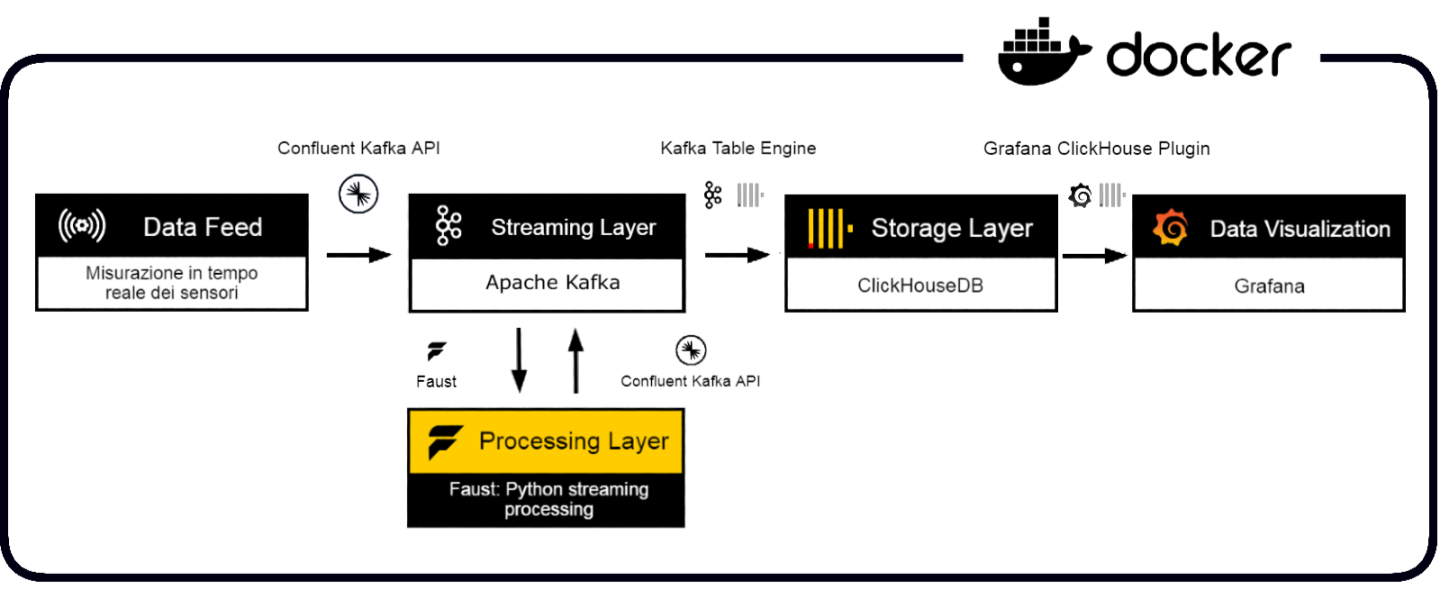
\includegraphics[width=1\textwidth]{../Images/SpecificaTecnica/Architettura_PB_microservices2.png}
    \caption{Componenti dell'architettura - Innovacity}
    \label{fig: fdf}
\end{figure}

\begin{itemize}
    \item \textbf{Data source}:Le sorgenti dati sono costituite da sensori IoT dislocati sul territorio cittadino. Questi sensori sono in grado di inviare, ad intervalli regolari, messaggi contenenti misurazioni allo streaming layer;
    \item \textbf{Streaming layer}:Lo streaming layer gestisce i dati in arrivo in tempo reale, per poi archiviarli sistematicamente nello \textit{storage}\textsubscript{\textit{G}} layer. Lo streaming Layer è composto da:
    \begin{itemize}
        \item \textbf{Apache Kafka}: \textit{Kafka}\textsubscript{\textit{G}} è un \textit{sistema}\textsubscript{\textit{G}} di messaggistica distribuito che consente di pubblicare, sottoscrivere e archiviare messaggi in tempo reale. \textit{Kafka}\textsubscript{\textit{G}} è utilizzato per ricevere i dati dai sensori IoT e renderli disponibili per l'elaborazione in tempo reale e batch.
        \item \textbf{Clickhouse Kafka table engine}:consumatore che legge i
        dati dal server \textit{Kafka}\textsubscript{\textit{G}} per persisterli nello \textit{storage}\textsubscript{\textit{G}} layer.
    \end{itemize}
    \item \textbf{Processing Layer:} Il processing Layer è costituito da Faust che consuma i dati dallo streaming layer e li processa in tempo reale. Faust è un \textit{framework}\textsubscript{\textit{G}} \textit{Python}\textsubscript{\textit{G}} che consente di scrivere applicazioni di streaming in tempo reale. Faust è utilizzato per elaborare i dati in arrivo tramite un modello per il calcolo del punteggio di salute che poi viene reso nuovamente disponibili allo streaming layer.
    \item \textbf{Storage layer}:Lo \textit{storage}\textsubscript{\textit{G}} layer è costituito da un \textit{database}\textsubscript{\textit{G}} column-oriented, \textit{ClickHouse}\textsubscript{\textit{G}}, che archivia i dati in arrivo dallo streaming layer. Questi dati sono disponibili per l'analisi e la visualizzazione in tempo reale e batch.
    \item \textbf{Data Visualization Layer}: composto da \textit{Grafana}\textsubscript{\textit{G}}, si occupa della visualizzazione dei dati elaborati ottenuti dallo \textit{storage}\textsubscript{\textit{G}} layer e della gestione delle notifiche in caso di anomalie rilevate.
\end{itemize}


\subsection{Data-flow}
Il diagramma rappresenta il percorso dei dati all'interno del sistema e le relative elaborazioni.

Vengono identificate le diverse entità coinvolte nel processo e le relazioni tra di esse, fornendo una panoramica dettagliata di come i dati vengono acquisiti, elaborati, archiviati e visualizzati.
\begin{figure}[H]
    \centering
    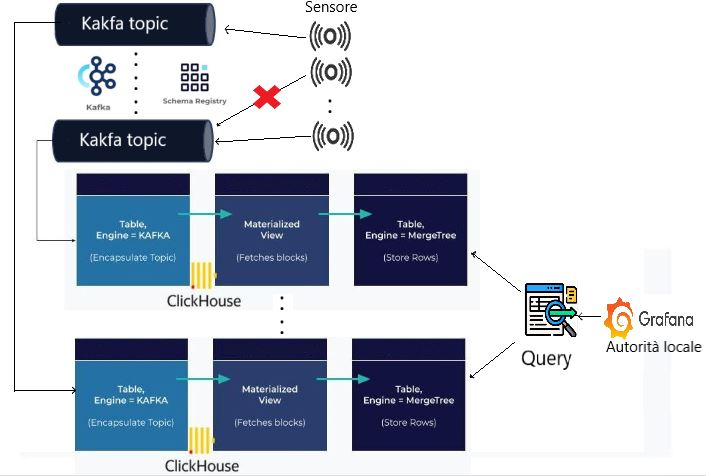
\includegraphics[width=1\textwidth]{../Images/SpecificaTecnica/data_flow.jpg}
    \caption{Data-flow - Innovacity}
    \label{fig: dataflow}
\end{figure}

\begin{enumerate}
    \item \textbf{Generazione e invio dati}:
    \begin{itemize}
        \item I dati vengono generati dai sensori IoT e inviati al broker Kafka.
    \end{itemize}
    
    \item \textbf{Serializzazione e diramazione}:
    \begin{itemize}
        \item I dati vengono serializzati secondo lo schema definito nello schema registry per il relativo topic.
        Nel caso in cui il formato del messaggio sia non conforme a quanto definito nello shcema registry questo viene scartato. A questo punto, il flusso si divide in due percorsi paralleli:
        \begin{enumerate}
            \item \textbf{Calcolo del punteggio di salute}:
            \begin{itemize}
                \item I dati di temperatura, umidità e polveri sottili vengono acquisiti da Faust per l'elaborazione.
                \item Faust applica il modello di calcolo del punteggio di salute e reinvia i dati processati a un topic dedicato in Kafka.
                \item Lo schema registry verifica la validità del messaggio prima dell'invio.
            \end{itemize}
            
            \item \textbf{Archiviazione}:
            \begin{itemize}
                \item Le misurazioni fluiscono verso ClickHouse tramite Kafka engine e materialized view per l'archiviazione.
            \end{itemize}
        \end{enumerate}
    \end{itemize}
    
    \item \textbf{Visualizzazione}:
    \begin{itemize}
        \item I dati archiviati in ClickHouse vengono interrogati da Grafana, che genera visualizzazioni per la loro presentazione.
    \end{itemize}
\end{enumerate}

\subsection{Architettura dei simulatori} \label{sec:architettura_simulatori}
Nonostante i simulatori non siano ufficialmente considerati come parte fondamentale del prodotto dalla proponente, ma necessari solamente per dimostrare il corretto funzionamento del sistema, il nostro team ha comunque scelto di dedicare alcune risorse alla progettazione di questa componente nell'ambito del progetto didattico.

Inoltre, abbiamo deciso di implementare e tenere conto delle possibili logiche dei microcontrollori associati ai sensori IoT, che possono effettuare operazioni per rendere più efficiente l'intero sistema.

Nei paragrafi successivi, verrà presentata l'architettura individuata mediante l'utilizzo di diagrammi delle classi e relative descrizioni. Inoltre, saranno motivate le scelte dei design pattern individuati e le decisioni progettuali rilevanti. Successivamente, per ogni classe, saranno illustrati metodi e attributi.

\subsubsection{Modulo simulatori sensori}
\begin{figure}[H]
    \centering
    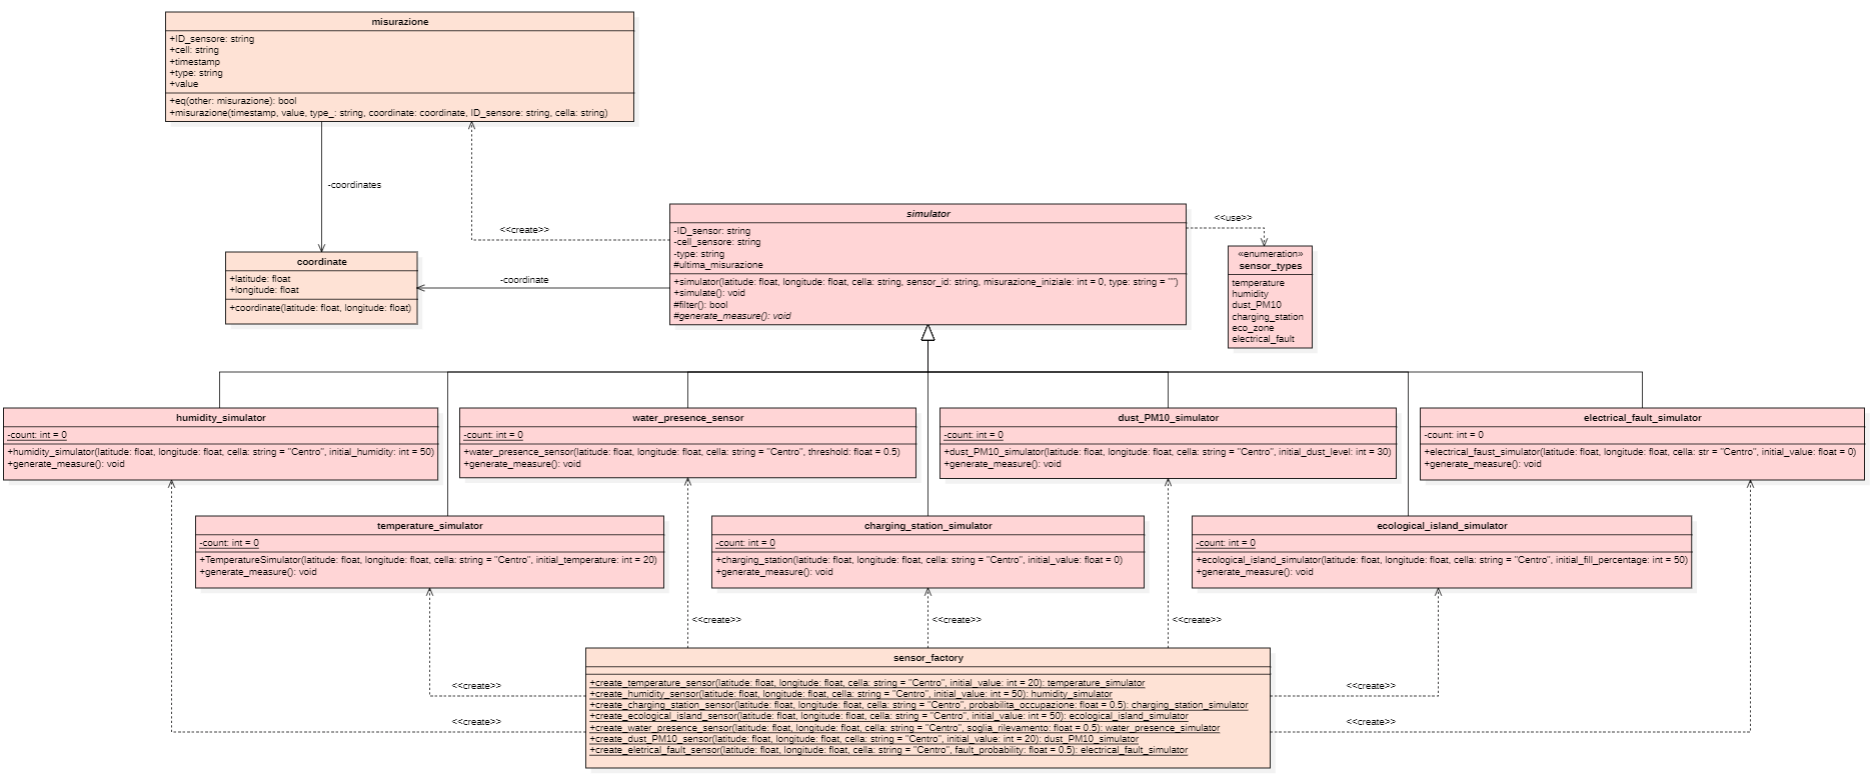
\includegraphics[width=1.1\textwidth]{../Images/SpecificaTecnica/simulatoriSensori.PNG}
    \caption{Modulo simulatori sensori - InnovaCity}
    \label{fig: Modulo_simulatori_sensori}
\end{figure}
Questo modulo si occupa della generazione di dati per diverse tipologie di sensori.
In particolare sono stati implementati simulatori per i seguenti tipi di sensori:
\begin{itemize}
    \item Sensori di temperatura;
    \item Sensori di umidità;
    \item Sensori di polveri sottili PM10;
    \item Sensori di stato occupazione colonnine di ricarica;
    \item Sensori di stato riempimento isole ecologiche;
    \item Sensori di presenza d'acqua;
    \item Sensori di guasto elettrico.
\end{itemize}
\paragraph{Design pattern Template Method} \label{sec:templateSIM}

La classe astratta \textit{simulator} implementa il design pattern \textit{Template Method}. Il metodo \textit{simulate()} fornisce lo scheletro dell'algoritmo per la generazione delle misurazioni e non può essere ridefinito nelle implementatazioni. Le classi che estendono \textit{simulator} implementano i metodi:
\begin{itemize}
    \item \textbf{\textit{generate\_measure()}:} Per la generazione semi-randomica della misurazione associata al tipo di sensore, di fatto non è richiesta una generazione di misurazioni realistiche dal prodotto, ma per poter avere una visualizzazione finale delle misurazioni non altalenanti ogni misurazione viene generata sulla base di quella precedente con una variazione limitata;
    
    \item \textbf{\textit{adapt()} - "hook method":} L'implementazione di default non modifica in alcun modo la misurazione generata. Può essere ridefinito per implementare la logica di adattamento della misurazione.
    
    Ad esempio:
    \begin{itemize}
        \item Per i sensori di polveri sottili PM10, la misurazione può essere adattata cambiando il valore dell'unità di misura µg/m³ in mg/m³ senza modifcare la logica di generazione in \textit{generate\_measure()};
        
        \item Per i sensori di temperatura, la misurazione può essere adattata cambiando il valore dell'unità di misura da °C a Fahrenheit  senza modifcare la logica di generazione in \textit{generate\_measure()};
        
        ~•~ Fahrenheit = (Celsius × 9/5) + 32
 
        \item Questo apre le porte alla possibilità di creare per una stessa tipoligia di sensore diverse implementazioni, che generano misurazioni con unità di misura diverse, senza dover modificare la logica di generazione che dichiara l'unità di misura generata di default, ma semplicemente estendendo la classe e ridefinendo il metodo \textit{adapt()} inserendo la formula di trasformazione.
        
    \end{itemize}
    \item Per garantire il rispetto del \textbf{Liskov Substitution Principle (LSP)} \textit{"Objects of a superclass should be replaceable with objects of its subtypes without altering the program's correctness."}:
    \begin{itemize}
        \item Il metodo \textit{adapt()} si limita a convertire le misurazioni senza alterare il comportamento generale del metodo \textit{simulate()} e senza modificare il tipo della misurazione generata da \textit{generate\_measure()};
        
        \item Il metodo \textit{generate\_measure()} viene reso \textbf{final} nelle concretizzazioni di \textit{simulator} impedendo la ridefinizione del comportamento.
    \end{itemize}

    In generale le postcondizioni sono piu forti nelle classi derivate, mentre non variano le precondizioni garantendo il rispetto di \textit{LSP}.
    
    Ad esempio:

    \begin{itemize}
        \item In \textit{simulator}:

        \begin{itemize}
            \item La postcondizione del metodo \textit{simulate()} in simulator è la generazione di un oggetto di tipo \textit{misurazione};
            
            \item La postcondizione del metodo \textit{generate\_measure} è la generazione del valore della misurazione.
            
            \item La postcondizione del metodo \textit{adapt()} è la possibilità di convertire il valore della misurazione.
        \end{itemize}

        \item In \textit{temperature\_simulator}, che eredita da \textit{simulator}:
        \begin{itemize}
            \item La postcondizione del metodo \textit{simulate()} è la generazione di un oggetto di tipo \textit{misurazione} di temperatura;
            
            \item La postcondizione del metodo \textit{generate\_measure} è la generazione del valore di una misurazione di temperatura;
            
            \item La postcondizione del metodo \textit{adapt()} è la possibilità di convertire il valore della misurazione ad un altra unità di misura (Kelvin, Fahrenheit).
        \end{itemize}

        \item In una possibile estensione futura \textit{temperature\_simulator\_fahrenheit}, che eredita da \textit{temperature\_simulator}:
        \begin{itemize}
            \item La postcondizione del metodo \textit{simulate()} è la generazione di un oggetto di tipo \textit{misurazione} di temperatura espresso in gradi Fahrenheit;
            
            \item La postcondizione del metodo \textit{generate\_measure} rimane invariata;
            
            \item La postcondizione del metodo \textit{adapt()} è di convertire il valore della misurazione dall'unità di misura di default a Fahrenheit.
        \end{itemize}
    \end{itemize}
\end{itemize}

Al termine delle operazioni di generazione e adattamento, il metodo \textit{simulate()} crea e restituisce un oggetto di tipo \textit{misurazione}.

Il design pattern \textit{Template Method} è stato scelto per:
\begin{itemize}
    \item Permettere una facile estensione del sistema con nuovi tipi di sensori che dovranno unicamente implementare la loro logica di generazione delle misurazioni e di adapting se necessario;
    
    \item Standardizzare i passi per la generazione delle misurazioni, garantendo coerenza e manutenibilità del codice;
    
    \item Ridurre la duplicazione del codice.
\end{itemize}

Come già esposto, una volta ottenuto lo stato del sensore, esso viene inserito in un oggetto di tipo \textit{misurazione}. Questo oggetto contiene informazioni di contesto come:
\begin{itemize}
    \item Identificativo del sensore;
    \item Cella della città in cui è presente il sensore;
    \item Timestamp della misurazione;
    \item Valore della misurazione;
    \item Coordinate;
    \item Tipologia di misurazione.
\end{itemize}

L'oggetto \textit{misurazione} viene poi ritornato al chiamante che si occuperà di inviarlo al server Kafka.
Un oggetto di tipo \textit{simulator} infatti, verrà assegnato ad ogni \textit{simulator\_thread}. Esso chiamerà ad intervalli regolari il metodo \textit{simulate()} ottenendo appunto la misurazione che invierà poi al server Kafka tramite un modulo apposito e indipendendente.

\paragraph{Design pattern Factory}
sensor\_factory implementa il design pattern \textit{Factory} per la creazione di simulatori dei sensori.
Il pattern \textit{Factory} è un pattern di tipo “Creazionale” secondo la classificazione della GoF.

I pattern di tipo creazionali si occupano della costruzione delle simulazioni dei sensori e delle problematiche che si possono originare, astraggono il processo di creazione degli oggetti, nascondono i dettagli della creazione e rendono i sistemi indipendenti da come gli oggetti sono creati e composti.

Il pattern \textit{Factory} incapsula la creazione concreta dei sensori, consentendo al client
(l’utilizzatore) di non conoscere i dettagli.

\paragraph{Classi, interfacce metodi e attributi:}
\begin{itemize}
    \item {\textbf{Classe astratta: \textit{simulator}}}
    \begin{itemize}
        \item \textbf{Attributi}: 
        \begin{itemize}
            \item \textbf{ID\_sensor: string [private]} - Identificatore univoco del sensore.
            \item \textbf{cella\_sensore: string [private]} - Identificatore della cella del sensore.
            \item \textbf{coordinate: coordinate [private]} - Coordinate geografiche del sensore.
            \item \textbf{misurazione: T [protected]} - Misurazione corrente del sensore.
            \item \textbf{type: string [private]} - Tipo di sensore.
        \end{itemize}
        \item \textbf{Metodi}:
        \begin{itemize}
            \item \textbf{simulate(): misurazione [public]} - Metodo principale per simulare la generazione di una misurazione.
            \item 
            Si basa sul design pattern Template Method:
            \begin{enumerate}
                \item Chiama generate\_measure() per generare un valore di misurazione.
                \item Chiama adapt() per effettuare adattamenti se necessari.
                \item Restituisce un oggetto \textit{misurazione} con data e ora corrente, valore misurato, tipo di sensore, coordinate e identificativo del sensore.
            \end{enumerate}
            \item \textbf{generate\_measure(): None [protected]} - Metodo astratto da implementare nelle classi concrete per generare un valore di misurazione semi-casuale coerente con la tipolgia di sensore da salvare nell'attributo \textit{misurazione}.
            \item \textbf{adapt(): void [protected]} - Fornisce un'implementazione di default che non modifica in alcun modo la misurazione generata. Può essere ridefinito per implementare la logica di adattamento della misurazione come conversioni di unità di misura.
        \end{itemize}
        \item \textbf{Note}:
        \begin{itemize}
            \item La classe \textit{simulator} è astratta e definisce il comportamento generale della simulazione della misurazione, pattern \textit{Template method}.
            \item Le classi concrete che ereditano da \textit{simulator} devono implementare il metodo astratto generate\_measure().
            \item Il metodo adapt() può essere ridefinito nelle classi concrete per implementare conversioni o adattamenti necessari.
            \item Il metodo \textit{simulate()} è final e non può essere ridefinito.
            \item Spiegazioni esaustive sono state presentate in: \ref{sec:templateSIM}
        \end{itemize}
    \end{itemize}
        
    \item{\textbf{Enumerazione: \textit{sensor\_types}}}
    \begin{itemize}
        \item \textbf{Costanti}: 
        \begin{itemize}
            \item \textbf{TEMPERATURE: string [public]} - Rappresenta la nomenclatura dei sensore di temperatura.
            \item \textbf{HUMIDITY: string [public]} - Rappresenta la nomenclatura dei sensore di umidità.
            \item \textbf{DUST\_PM10: string [public]} - Rappresenta la nomenclatura dei sensore di "polvere PM10".
            \item \textbf{CHARGING\_STATION: string [public]} - Rappresenta la nomenclatura dei sensore di stato delle colonnine di ricarica.
            \item \textbf{ECOLOGICAL\_ISLAND: string [public]} - Rappresenta la nomenclatura dei sensore di stato riempimento isole ecologica.
            \item \textbf{WATER\_PRESENCE: string [public]} - Rappresenta la nomenclatura dei sensore di presenza d'acqua.
            \item \textbf{ELECTRICAL\_FAULT: string [public]} - Rappresenta la nomenclatura dei sensore di guasti elettrici.
        \end{itemize}

        \item \textbf{Note}:
        \begin{itemize}
            \item L'enumerazione viene utilizzata per centralizzare la gestione della nomenclatura dei tipi di sensori che verrà salvata nelle misurazioni.
        \end{itemize}
    \end{itemize}
        
    \item{\textbf{Classe: \textit{temperature\_simulator}}}
    \begin{itemize}
        \item \textbf{Attributi:}
        \begin{itemize}
            \item \textbf{count: int [private, static]} - Contatore statico per generare un ID univoco per ogni istanza.
        \end{itemize}
        \item\textbf{Metodi}: 
        \begin{itemize}
            \item \textbf{generate\_measure(): None [protected,final]} - Genera una misurazione di temperatura in gradi Celsius semi-casuale e aggiorna lo stato interno con il valore della misurazione corrente.
        \end{itemize}
        \item\textbf{Note}:
        \begin{itemize}
            \item La classe \textit{temperature\_simulator} è una classe concreta che eredita dalla classe astratta \textit{simulator}.
            \item Il costruttore genera automaticamente un ID sensore univoco per ogni istanza.
            \item Dichiara di generare misurazioni di temperatura con unità di default (Gradi Celsius), possibili classi derivate possono effettuare conversioni ad altre unità di misura (Kelvin,Fahrenheit) tramite il metodo \textit{adapt()}, senza dover modificare la logica di generazione.
        \end{itemize}
    \end{itemize}
    
    \item{\textbf{Classe: \textit{humidity\_simulator}}}
    \begin{itemize}
        \item\textbf{Attributi:}
        \begin{itemize}
            \item \textbf{count: int [private, static]} - Contatore statico per generare un ID univoco per ogni istanza.
        \end{itemize}
        \item \textbf{Metodi}: 
        \begin{itemize}
            \item \textbf{generate\_measure(): None [protected,final]} - Genera una misurazione di umidità in percentuale semi-casuale e aggiorna lo stato interno con il valore della misurazione corrente.
        \end{itemize}
        \item \textbf{Note}:
        \begin{itemize}
        \item La classe \textit{humidity\_simulator} è una classe concreta che eredita dalla classe astratta \textit{simulator}.
        \item Il costruttore genera automaticamente un ID sensore univoco per ogni istanza.
        \item Dichiara di generare misurazioni di umidità con unità di default (Percentuale), possibili classi derivate possono effettuare conversioni ad altre unità di misura (g/m³) tramite il metodo \textit{adapt()}, senza dover modificare la logica di generazione.
        \end{itemize}
    \end{itemize}

    \item{\textbf{Classe: \textit{charging\_station\_simulator}}}
    \begin{itemize}
        \item \textbf{Attributi}: 
        \begin{itemize}
            \item \textbf{count: int [private, static]} - Contatore statico per generare un ID univoco per ogni istanza.
        \end{itemize}
        \item \textbf{Metodi}:
        \begin{itemize}
            \item \textbf{generate\_measure(): None [protected,final]} - Genera lo stato della colonnina di ricarica (Occupato: \textsc{True}, Libero: \textsc{False}) basata su una probabilità di transizione e aggiorna lo stato interno con il valore della misurazione corrente.
        \end{itemize}
        \item \textbf{Note}:
        \begin{itemize}
            \item La classe \textit{charging\_station\_simulator} è una classe concreta che eredita dalla classe astratta \textit{simulator}.
            \item Il costruttore genera automaticamente un ID sensore univoco per ogni istanza.
            \item Implementa il metodo astratto \textit{generate\_measure()} per generare una misurazione basata sulla probabilità di transizione.
        \end{itemize}
    \end{itemize}

    \item{\textbf{Classe: \textit{dust\_PM10\_simulator}}}
    \begin{itemize}
        \item \textbf{Attributi}: 
        \begin{itemize}
            \item \textbf{count: int [private, static]} - Contatore statico per generare un ID univoco per ogni istanza.
        \end{itemize}
        \item \textbf{Metodi}: 
        \begin{itemize}
            \item \textbf{generate\_measure(): None [protected,final]} - Genera una variazione di quantità di polvere PM10 semi-casuale e aggiorna lo stato interno con il valore della misurazione corrente.
        \end{itemize}
        \item \textbf{Note}:
        \begin{itemize}
            \item La classe \textit{dust\_PM10\_simulator} è una classe concreta che eredita dalla classe astratta \textit{simulator}.
            \item Il costruttore genera automaticamente un ID sensore univoco per ogni istanza.
            \item Dichiara di generare misurazioni di polvere PM10 in con unità di default (µg/m³), possibili classi derivate possono effettuare conversioni ad altre unità di misura (mg/m³) tramite il metodo \textit{adapt()}, senza dover modificare la logica di generazione.
        \end{itemize}
    \end{itemize}

    \item{\textbf{Classe: \textit{electrical\_fault\_simulator}}}
    \begin{itemize}
        \item \textbf{Attributi}: 
        \begin{itemize}
            \item \textbf{count: int [private, static]} - Contatore statico per generare un ID univoco per ogni istanza.
        \end{itemize}
        \item \textbf{Metodi}: 
        \begin{itemize}
            \item \textbf{generate\_measure(): None [protected,final]} - Genera lo stato di una centralina elettrica (Guasto verificato: \textsc{True}, Operativa: \textsc{False}) basandosi su una probabilità di guasto e aggiorna lo stato interno con il valore della misurazione corrente.
        \end{itemize}
        \item \textbf{Note}:
        \begin{itemize}
            \item La classe \textit{electrical\_fault\_simulator} è una classe concreta che eredita dalla classe astratta \textit{simulator}.
            \item Il costruttore genera automaticamente un ID sensore univoco per ogni istanza.
        \end{itemize}
    \end{itemize}

    \item{\textbf{Classe: \textit{ecological\_island\_simulator}}}
    \begin{itemize}
        \item \textbf{Attributi}: 
        \begin{itemize}
            \item \textbf{count: int [private, static]} - Contatore statico per generare un ID univoco per ogni istanza.
        \end{itemize}
        \item \textbf{Metodi}: 
        \begin{itemize}
            \item \textbf{generate\_measure(): None [protected,final]} - Genera una misurazione della percentuale di riempimento di un isola ecologica e aggiorna lo stato interno con il valore della misurazione corrente.
        \end{itemize}
        \item \textbf{Note}:
        \begin{itemize}
            \item La classe \textit{ecological\_island\_simulator} è una classe concreta che eredita dalla classe astratta \textit{simulator}.
            \item Il costruttore genera automaticamente un ID sensore univoco per ogni istanza.
        \end{itemize}
    \end{itemize}

    \item{\textbf{Classe: \textit{water\_presence\_sensor}}}
    \begin{itemize}
        \item \textbf{Attributi}: 
        \begin{itemize}
            \item \textbf{count: int [private, static]} - Contatore statico per generare un ID univoco per ogni istanza.
        \end{itemize}
        \item \textbf{Metodi}: 
        \begin{itemize}
            \item \textbf{generate\_measure(): None [protected,final]} - Genera una misurazione basata sulla soglia di presenza dell'acqua (Acqua rilevata: \textsc{True}, Acqua non rilevata: \textsc{False}) e aggiorna lo stato interno con il valore della misurazione corrente.
        \end{itemize}
        \item \textbf{Note}:
        \begin{itemize}
            \item La classe \textit{ecological\_island\_simulator} è una classe concreta che eredita dalla classe astratta \textit{simulator}.
            \item Il costruttore genera automaticamente un ID sensore univoco per ogni istanza.
        \end{itemize}
    \end{itemize}

    \item{\textbf{Classe: \textit{misurazione}}}
    \begin{itemize}
        \item \textbf{Attributi}: 
        \begin{itemize}
            \item \textbf{timestamp: datetime [private]} - Timestamp della misurazione.
            \item \textbf{value: T [private]} - Valore della misurazione.
            \item \textbf{type: string [private]} - Tipo della misurazione.
            \item \textbf{coord: coordinate [private]} - Coordinate della misurazione.
            \item \textbf{ID\_sensore: string [private]} - ID del sensore che ha effettuato la misurazione.
            \item \textbf{cella: string [private]} - Cella in cui è stata effettuata la misurazione.
        \end{itemize}
        \item \textbf{Metodi}: 
        \begin{itemize}
            \item \textbf{\_\_eq\_\_(other: misurazione): bool [public]} - Ridefinizione dell'operatore di uguaglianza per confrontare due oggetti \textit{misurazione}.
        \end{itemize}
    \end{itemize}

    \item{\textbf{Classe: \textit{coordinate}}}
    \begin{itemize}
        \item \textbf{Attributi}: 
        \begin{itemize}
            \item \textbf{latitude: float [private]} - Latitudine della coordinata.
            \item \textbf{longitude: float [private]} - Longitudine della coordinata.
        \end{itemize}
        \item \textbf{Metodi}: 
        \begin{itemize}
            \item \textbf{\_\_eq\_\_(other: coordinate):bool [public]} - Ridefinizione dell'operatore di uguaglianza per confrontare due oggetti \textit{coordinate}.
        \end{itemize}
    \end{itemize}

    \item{\textbf{Classe: \textit{sensor\_factory}}}
    \begin{itemize}
        \item \textbf{Metodi}: 
        \begin{itemize}
            \item \textbf{create\_temperature\_sensor(latitude: float, longitude: float, cella: string, initial\_value: float): temperature\_simulator [public, static]} - Crea un simulatore di temperatura.

            \item \textbf{create\_humidity\_sensor(latitude: float, longitude: float, cella: string, initial\_value: float): humidity\_simulator [public, static]} - Crea un simulatore di umidità.
            
            \item \textbf{create\_charging\_station\_sensor(latitude: float, longitude: float, cella: string, probabilita\_occupazione: float): charging\_station\_simulator [public, static]} - Crea un simulatore di stazione di ricarica.
            
            \item \textbf{create\_ecological\_island\_sensor(latitude: float, longitude: float, cella: string, initial\_value: float): ecological\_island\_simulator [public, static]} - Crea un simulatore di isola ecologica.
            
            \item \textbf{create\_water\_presence\_sensor(latitude: float, longitude: float, cella: string, soglia\_rilevamento: float): water\_presence\_sensor [public, static]} - Crea un sensore di presenza d'acqua.
            
            \item \textbf{create\_dust\_PM10\_sensor(latitude: float, longitude: float, cella: string, initial\_value: float): dust\_PM10\_simulator [public, static]} - Crea un simulatore di polvere PM10.
            
            \item \textbf{create\_eletrical\_fault\_sensor(latitude: float, longitude: float, cella: string, fault\_probability: float): electrical\_fault\_simulator [public, static]} - Crea un simulatore di guasto elettrico.
        \end{itemize}
    \textbf{Note}:
        \begin{itemize}
            \item Implementazione del pattern Factory;
            \item Fornisce metodi per la creazione di simulatori di sensori;
            \item Astrae il processo di creazione dei sensori, nascondendo i dettagli della creazione.
        \end{itemize}
    \end{itemize}
\end{itemize}

\subsubsection{Modulo Writers} \label{sec:writersModule}

\begin{figure}[H]
    \centering
    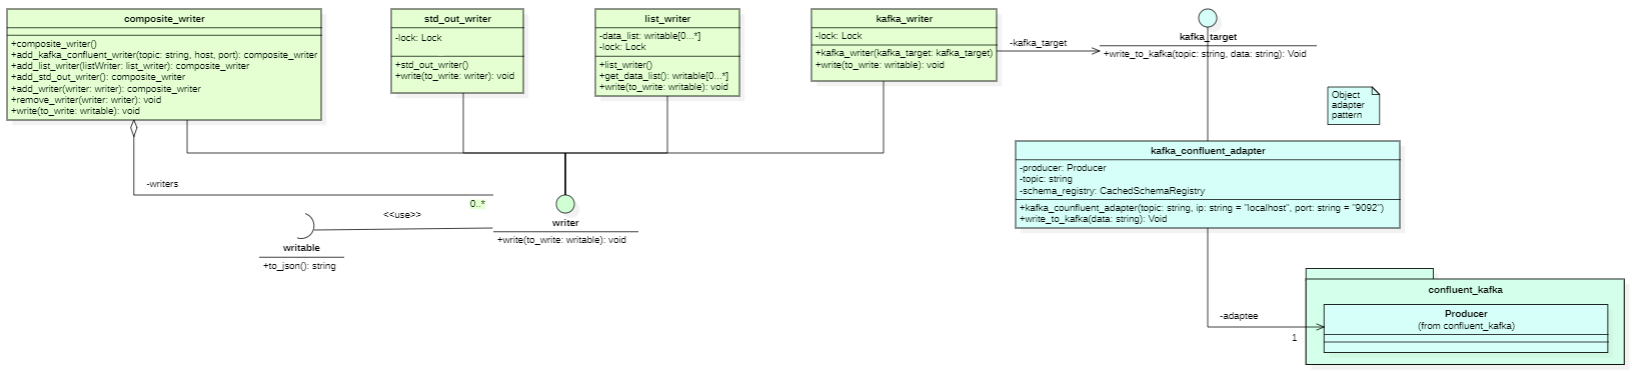
\includegraphics[width=1.1\textwidth]{../Images/SpecificaTecnica/writerModule.PNG}
    \caption{Modulo writers - InnovaCity}
    \label{fig: writersModule}
\end{figure}

Questo modulo si occupa della scrittura e/o invio di informazioni a diverse tipologie di servizi e vuole essere completamentemente indipendendente e non influenzato dal modulo della simulazione dei sensori, così da poter consentire un suo riutilizzo.
Per quanto riguarda la scrittura in Kafka, l'impiego della connessione allo Schema Registry (vedi sezione \S\ref{sec:schema_registry}) consente la convalida del formato del messaggio prima della sua scrittura nei topic Kafka. Questa pratica permette di ridurre il carico di rete nel caso di messaggi malformati, consentendo un filtraggio "alla fonte".

\paragraph{Design pattern Strategy + Composite:}
Il modulo presenta un'interfaccia \textit{writer} che offre il metodo di scrittura \textit{write()} di oggetti che implementano \textit{writable}.
Questo metodo è implementato da diverse classi concrete che rappresentano i vari servizi a cui è possibile inviare le informazioni.
L'approccio adottato implementa il design pattern \textit{Strategy} per la scrittura/invio dei dati su diverse piattaforme/servizi e il design pattern \textit{Composite} per la scrittura ad uno o più servizi in modo uniforme.
Nello specifico sono state implentate tre strategie di scrittura: la prima, (\textit{kafka\_writer}), atta a permettere al simulatore di inviare messaggi a topic Kafka,  la seconda (\textit{std\_out\_writer}) atta a permettere di stampare gli \textit{writable} su terminale e la terza (\textit{list\_writer}) per il salvataggio su una lista degli \textit{writable}.
L'utilizzo del design pattern Composite e Strategy in questo caso ha diverse motivazioni:

\begin{enumerate}
    \item \textit{kafka\_writer}, atta a permettere al simulatore di inviare messaggi a Kafka;
    \item \textit{std\_out\_writer}, atta a permettere di stampare i \textit{writable} su terminale;
    \item \textit{list\_writer} per il salvataggio su una lista degli oggetti di tipo \textit{writable}.
\end{enumerate}
L'utilizzo dei design pattern Composite e Strategy in questo caso ha diverse motivazioni:
\begin{itemize}
    \item \textbf{Gestione uniforme dei servizi}: Il pattern Strategy consente di definire una famiglia di algoritmi, incapsularli e renderli intercambiabili. In questo caso, i servizi di scrittura sono trattati come algoritmi intercambiabili, consentendo di scrivere informazioni su diversi servizi senza dover conoscere i dettagli di implementazione di ciascuno.
    \item \textbf{Gestione gerarchica dei servizi}: Il pattern Composite consente di trattare gli oggetti singoli e le loro composizioni (gruppi di oggetti) allo stesso modo. \\
    Nel contesto del modulo, potrebbe esserci la necessità di gestire non solo singoli servizi, ma anche gruppi di servizi. Ad esempio, potrebbe essere utile inviare informazioni al servizio Kafka e contemporaneamente stamparle nel terminale e memorizzarle in un'apposita lista per il testing. Il Composite consente di comporre questi servizi in modo gerarchico e trattarli uniformemente.
\end{itemize}

\paragraph{Design pattern Object Adapter:}
Nello specifico, la classe \textit{kafka\_writer} realizza la sua funzionalità attraverso l'utilizzo del design pattern \textit{Adapter}, nella sua variante \textit{Object Adapter}. Tale scelta è stata motivata dall'impiego della classe \textit{Producer} della libreria \textit{confluent\_kafka}, la quale potrebbe subire variazioni non controllabili da noi. Per garantire la capacità di rispondere prontamente a tali cambiamenti senza dover modificare la classe \textit{kafka\_writer} o altri parti di sistema, si è optato per l'utilizzo di questo pattern, trasferendo così la complessità derivante da tali modifiche proprio nell'adapter.
Inoltre grazie all'interfaccia \textit{kafka\_target}, si è garantita la possibilità di estendere il sistema con nuovi metodi di scrittura su Kafka o l'utilizzo di nuove librerie senza dover modificare la classe \textit{kafka\_writer} ma solamente aggiungendo una nuova classe adapter che implementi \textit{kafka\_target}.

\paragraph{Classi: metodi e attributi}

\begin{itemize}
    \item{\textbf{Interfaccia: \textit{writable}}}
    \begin{itemize}
        \item\textbf{Metodi}: 
        \begin{itemize}
            \item \textbf{to\_json(): string [public, abstract]} - Metodo astratto che deve essere implementato nelle sottoclassi per convertire l'oggetto in una stringa JSON.
        \end{itemize}
        \item\textbf{Note}:
        \begin{itemize}
            \item L'interfaccia \textit{writable} definisce un insieme di metodi che una classe deve implementare perchè possa essere utilizzata dalle strategie di scrittura.
        \end{itemize}
    \end{itemize}
    \item{\textbf{Interfaccia: \textit{writer}}}
     \begin{itemize}
        \item \textbf{Metodi:}
         \begin{itemize}
            \item \textbf{write(to\_write: writable): None [public, abstract]} - Metodo astratto che deve essere implementato nelle sottoclassi per scrivere un oggetto writable.
        \end{itemize}
        \item\textbf{Note}:
        \begin{itemize}
            \item L'interfaccia \textit{writer} definisce il metodo che una classe deve implementare perchè possa essere utilizzata come strategia di scrittura. Rappresenta il componente "\textit{strategy}" del pattern "\textit{Strategy}";
            \item Rappresenta l'interfaccia "\textit{Component}" del pattern \textit{Composite} che descrive le operazioni comuni sia agli elementi semplici che a quelli complessi dell'albero.
        \end{itemize}
    \end{itemize}
    \item{\textbf{Classe: \textit{composite\_writer}}}
    \begin{itemize}
    \item\textbf{Attributi}:
        \begin{itemize}
        \item \textbf{writers: writer [private]} - Lista di oggetti \textit{writer}.
    \end{itemize}
    \item \textbf{Metodi: }
    \begin{itemize}
        \item \textbf{add\_writer(writer: ): composite\_writer [public]} - Aggiunge un oggetto che implementa \textit{writer} alla lista writers.
        \item \textbf{add\_kafka\_confluent\_writer(topic: string, host: string, port: int, schema\_registry\_url: string): composite\_writer [public]} - Crea un \textit{kafka\_writer} con un \textit{kafka\_confluent\_adapter} e lo aggiunge alla lista writers. Ritorna se stesso per permettere operazione concatenate.
        \item \textbf{add\_stdOut\_writer(): composite\_writer [public]} - Crea un \textit{std\_out\_writer} e lo aggiunge alla lista writers. Ritorna se stesso per permettere operazione concatenate.
        \item \textbf{add\_list\_writer(writer\_list: list\_writer): composite\_writer [public]} - Aggiunge un \textit{list\_writer} alla lista writers. Ritorna se stesso per permettere operazione concatenate.
        \item \textbf{remove\_writer(writer: writer): composite\_writer [public]} - Rimuove un \textit{writer} dalla lista writers.  Ritorna se stesso per permettere operazione concatenate.
        \item \textbf{write(to\_write: writable): \textit{composite\_writer} [public]} - Chiama il metodo write su ogni writer nella lista writers passando come attributo il \textit{writable} ricevuto.
    \end{itemize}
    \item\textbf{Note}:
        \begin{itemize}
            \item La classe è la componente "Composite" del pattern \textit{Composite}, ovvero l'elemento che può avere sottoelementi;
            \item Dopo aver ricevuto una richiesta, il contenitore (detto composite) delega il lavoro ai suoi sottoelementi: foglie o altri contenitori.
        \end{itemize}
    \end{itemize}
    \item{\textbf{Classe: \textit{std\_out\_writer}}}
    \begin{itemize}
    \item\textbf{Attributi}:
        \begin{itemize}
        \item \textbf{lock:threading.Lock [private]} - Lock per garantire l'accesso esclusivo alla stampa ed un esecuzione Thread safe.
    \end{itemize}
    \item \textbf{Metodi: }
    \begin{itemize}
        \item \textbf{write(to\_write: writable): None [public]} - Stampa l'oggetto writable come stringa JSON nella console;
    \end{itemize}
    \item\textbf{Note}:
        \begin{itemize}
            \item La classe è una strategia di scrittura del pattern \textit{Strategy} ma anche la componente "Leaf" del pattern \textit{Composite}, ovvero l'elemento base che non ha sottoelementi.
        \end{itemize}
    \end{itemize}
    \item{\textbf{Classe: \textit{list\_writer}}}
    \begin{itemize}
    \item\textbf{Attributi}:
        \begin{itemize}
        \item \textbf{data\_list:list [private]} - Lista per memorizzare gli oggetti writable.
        \item \textbf{lock:threading.Lock [private]} - Lock per garantire l'accesso esclusivo alla lista ed un esecuzione Thread safe.
    \end{itemize}
    \item \textbf{Metodi: }
    \begin{itemize}
        \item \textbf{write(to\_write: writable): None [public]} - Aggiunge l'oggetto writable alla lista.
        \item \textbf{get\_data\_list(): list [public]} - Restituisce la lista di oggetti writable.
    \end{itemize}
    \item\textbf{Note}:
        \begin{itemize}
            \item La classe è una strategia di scrittura del pattern \textit{Strategy} ma anche la componente "Leaf" del pattern \textit{Composite}, ovvero l'elemento base che non ha sottoelementi.
        \end{itemize}
    \end{itemize}
    \item{\textbf{Classe: \textit{kafka\_writer}}}
    \begin{itemize}
    \item\textbf{Attributi}:
        \begin{itemize}
        \item \textbf{lock:threading.Lock [private]} - Lock per garantire l'accesso esclusivo alla scrittura su Kafka ed un esecuzione Thread safe.
        \item \textbf{kafka\_target:kafka\_target [private]} - Riferimento ad un implementazione di kafka\_target per effettuare l'effettiva scrittura in Kafka tramite librerie.
    \end{itemize}
    \item \textbf{Metodi: }
    \begin{itemize}
        \item \textbf{write(to\_write: writable): None [public]} - Scrive l'oggetto \textit{writable} come stringa JSON su Kafka.
    \end{itemize}
    \item\textbf{Note}:
        \begin{itemize}
            \item La classe è una strategia di scrittura del pattern \textit{Strategy} ma anche la componente "Leaf" del pattern \textit{Composite}, ovvero l'elemento base che non ha sottoelementi.
            \item La costruzione dell'oggetto \textit{kafka\_writer} richiede un riferimento ad un oggetto che implementi l'interfaccia kafka\_target.
        \end{itemize}
    \end{itemize}
    \item{\textbf{Interfaccia: kafka\_target}}
    \begin{itemize}
        \item \textbf{Metodi: }
        \begin{itemize}
            \item \textbf{write\_to\_kafka(data: string): None [public, abstract]} - Metodo astratto che deve essere implementato nelle sottoclassi per scrivere dati su Kafka.
        \end{itemize}
        \item\textbf{Note}:
        \begin{itemize}
            \item La classe è una interfaccia che fornisce un contratto per le operazioni di scrittura/invio a topic Kafka.
            \item Rappresenta il componente Target del pattern \textit{Object Adapter}.
        \end{itemize}
    \end{itemize}
    \item{\textbf{Classe: \textit{KafkaConfluentAdapter}}}
    \begin{itemize}
        \item\textbf{Attributi}:
        \begin{itemize}
            \item \textbf{topic:string [private]} - Il topic su cui scrivere in Kafka;
            \item \textbf{producer:Producer [private]} - Il producer Kafka per inviare messaggi;
            \item \textbf{schema\_registry:CachedSchemaRegistryClient [private]} - Consente di interagire con Confluent Schema Registry in modo efficiente, memorizza in cache gli schemi recuperati da Schema Registry, riducendo le chiamate di rete e migliorando la velocità di accesso agli schemi.
        \end{itemize}
    \end{itemize}
    \item \textbf{Metodi: }
    \begin{itemize}
        \item \textbf{write\_to\_kafka(data: string): None [public]} - Scrive i dati su Kafka dopo averli validati rispetto allo schema registrato per il topic di destinazione.
    \item\textbf{Note}:
        \begin{itemize}
            \item La classe è un'implementazione concreta dell'interfaccia \textit{kafka\_target}, utilizzando la libreria \textit{confluent-kafka} per interagire con Kafka;
            \item Rappresenta il componente "Adapter" del pattern \textit{Object Adapter};
            \item Il Producer kafka rappresenta la componente "service" del pattern \textit{Object Adapter};
            \item Prima di inviare il messaggio (ovvero la misurazione) controlla che sia nel formato/schema corretto per il topic di destinazione evintando cosi sovraccarico inutile di rete;
            \item Nel caso in cui il formato del messaggio sia scorretto questo viene scartato.
        \end{itemize}
    \end{itemize}
\end{itemize}

\subsubsection{Modulo Threading/Scheduling}
\begin{figure}[H]
    \centering
    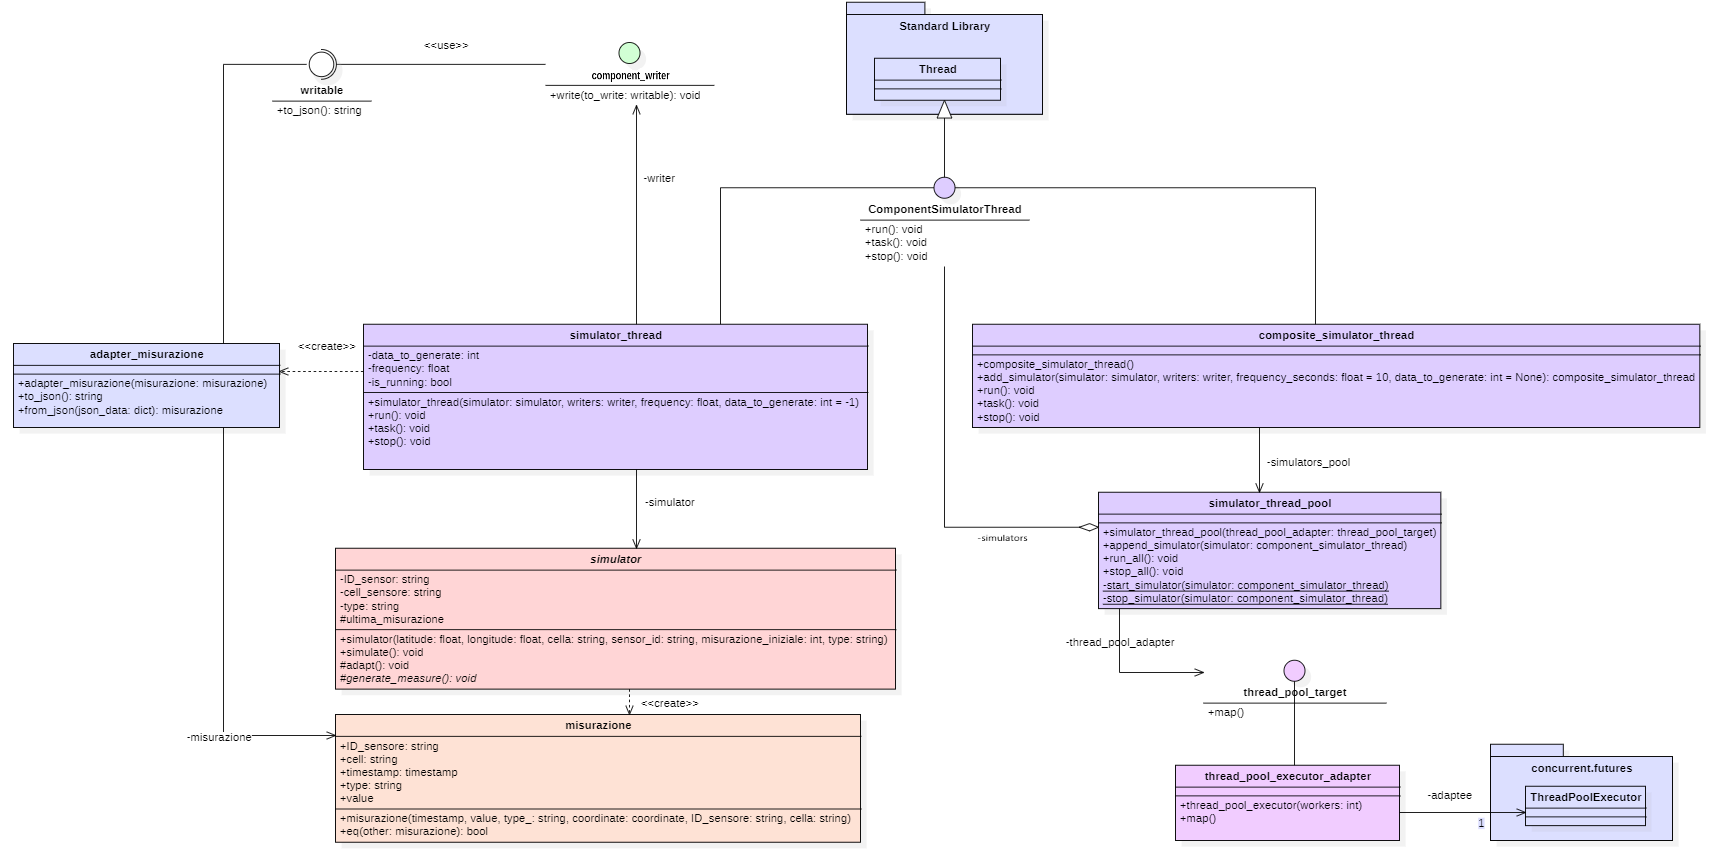
\includegraphics[width=1.1\textwidth]{../Images/SpecificaTecnica/simulatorThread.PNG}
    \caption{Modulo Threading/Scheduling simulatori sensori - InnovaCity}
    \label{fig: Modulo_simulatori_sensori_thread}
\end{figure}
Questo modulo si propone di gestire la logica di pianificazione per il recupero dei dati dai simulatori dei sensori e di inviare/scrivere tali dati utilizzando il modulo Writer. Funge da orchestratore per i due moduli appena descritti, offrendo la possibilità di configurare la frequenza di campionamento o il numero di misurazioni da eseguire. Inoltre, incorpora una logica di ottimizzazione, simile a quella impiegata dai microcontrollori dei sensori nella realtà, al fine di evitare la trasmissione di dati ridondanti, inviando solo i cambiamenti di stato dei sensori.

\paragraph*{Dependecy Inversion principle}
Il modulo è stato progettato per rispettare il principio di inversione delle dipendenze. Infatti, la classe \textit{simulator\_thread\_pool} è stata progettata per essere indipendente dalla libreria di gestione dei thread utilizzata, consentendo di sostituirla senza dover modificare il codice di \textit{simulator\_thread\_pool}.
Inoltre, i componenti del modulo sono progettati per essere indipendenti dai dettagli di implementazione dei simulatori e degli "writers", consentendo di sostituire i simulatori e gli "writers" senza dover modificare il codice.
In sintesi, i moduli di alto livello (Modulo Writer e simulatori) non dipendono da moduli di basso livello che incorporano funzioni di utilità.(Modulo Threading)
Sia i moduli di alto livello che quelli di basso livello dipendono da astrazioni (interfacce o classi astratte).


\paragraph{Design pattern Composite:}
Come per il modulo di scrittura anche questo è sviluppato secondo il pattern Composite che permette di gestire un singolo Thread di esecuzione o un gruppo di Thread in modo uniforme.
\paragraph{Design pattern Object Adapter:}
Inoltre, considerando l'impiego di più thread per un esecuzione parallela, per delegare l'orchestrazione delle operazioni, si è fatto ricorso alle ThreadPool. Al fine di evitare modifiche dirette al codice di \textit{simulator\_thread\_pool}, è stato adottato il pattern \textit{Object Adapter} per adattare la ThreadPool di Python a un'interfaccia comune con cui \textit{simulator\_thread\_pool} possa interagire. Questo approccio consente di modificare la logica o la libreria utilizzata per la gestione dei thread senza richiedere modifiche al codice di \textit{simulator\_thread\_pool}, ma semplicemente aggiungendo una nuova classe adapter che implementi \textit{thread\_pool\_target}.

Un'altra implementazione del pattern \textit{Object Adapter} viene impiegata per adattare gli oggetti \textit{misurazione} del modulo dei \textit{Simulatori} agli oggetti \textit{writable} del modulo \textit{Writers}. La classe \textit{adapter\_misurazione}, implementando l'interfaccia \textit{writable}, fornisce un'implementazione del metodo \textit{to\_json()} che consente di convertire un oggetto \textit{misurazione} nel formato JSON, compatibile con il formato definito nello Schema Registry e riconosciuto da Kafka.
\ref*{sec:formatoMessaggi}


\paragraph{Classi: metodi e attributi}

\begin{itemize}
    \item{\textbf{Interfaccia: \textit{component\_simulator\_thread}}}
    \begin{itemize}
        \item \textbf{Metodi: }
        \begin{itemize}
            \item \textbf{run(): None [public, abstract]} - Metodo astratto che deve essere implementato nelle sottoclassi per definire il comportamento del thread quando viene avviato.
            \item \textbf{task(): None [public, abstract]} - Metodo astratto che deve essere implementato nelle sottoclassi per definire il compito specifico che il thread deve eseguire.
            \item \textbf{stop(): None [public, abstract]} - Metodo astratto che deve essere implementato nelle sottoclassi per definire come fermare il thread.
        \end{itemize}
        \item\textbf{Note}:
        \begin{itemize}
            \item Eredita le proprietà e i metodi della classe \textit{Thread} della \textit{Standard Library};
            \item \textit{component\_simulator\_thread} è un interfaccia di threading per la simulazione sensori, fornendo un contratto per le operazioni di avvio, esecuzione del compito e arresto;
            \item Rappresenta il componente "Component" del pattern \textit{Composite},descrive le operazioni comuni sia ai singoli Thread sia a composizioni di questi;
            \item L'utilizzatore dei simulatori può lavorare allo stesso modo con elementi semplici (singoli Thread) o complessi (insiemi di Thread in forma di albero).
        \end{itemize}
    \end{itemize}
    \item{\textbf{Classe: \textit{simulator\_thread}}}
    \begin{itemize}
        \item\textbf{Attributi}:
        \begin{itemize}
            \item \textbf{simulator:\textit{simulator} [private]} - Il simulatore da utilizzare per generare i dati.
            \item \textbf{frequency:float [private]} - La frequenza con cui generare i dati.
            \item \textbf{is\_running:bool [private]} - Flag per controllare se il thread è in esecuzione.
            \item \textbf{data\_to\_generate:int [private]} - Il numero di dati da generare.
            \item \textbf{writers:writer [private]} - L'oggetto implementazione di \textit{writer} per scrivere i dati generati. (Singolo o albero - Composite pattern)
        \end{itemize}
        \item \textbf{Metodi: }
        \begin{itemize}
            \item \textbf{run(): None [public]} - Avvia il thread del simulatore.
            \item \textbf{task(): None [public]} - Definisce il compito specifico che il thread deve eseguire, contiene la logica per generare il numero di misurazioni richieste con l'intervallo specificato alla costruzione.
            Inoltre evita l'invio di misurazioni consecutive uguali cosi da ridurre il carico scartando dati ridondanti e deducibili inviando agli \textit{"Writers"} solo i cambi di stato del sensore da cui acquisisce la misurazione.
            All'interno del metodo, la misurazione restituita dal simulatore, viene adattata ad un oggetto \textit{writable} tramite \textit{adapter\_misurazione} ed inviata agli \textit{"Writers"}.
            \item \textbf{stop(): None [public]} - Ferma il thread del simulatore.
        \end{itemize}
        \item\textbf{Note}:
        \begin{itemize}
            \item La classe è un'implementazione concreta dell'interfaccia \textit{component\_simulator\_thread};
            \item Utilizza un oggetto \textit{\textit{simulator}} per generare dati a una certa frequenza e un oggetto che implementa\textit{component\_writer} per scrivere i dati generati;
            \item Rappresenta il componente Leaf del pattern \textit{Composite};
            \item Se data\_to\_generate < 0 => Genera misurazioni finchè il thread non viene interroto dall'esterno.
            \item Sebbene i simulatori non siano considerati dalla proponente parte del prodotto, la logica di ottimizzazione per inviare solo i cambi di stato dei sensori viene implementata nella realtà IoT. Di conseguenza, è stata presa la decisione di replicarla. È importante notare che questa logica non è incorporata nel Simulatore del sensore, il quale ha unicamente il compito semantico di generare dati come un vero sensore. Invece, essa è implementata in \textit{simulator\_thread}, il quale agisce in modo simile a un microcontrollore, responsabile sia della gestione dell'intervallo di campionamento che della logica per l'invio delle misurazioni;
            \item Nel corso dello sviluppo futuro, potrebbe risultare vantaggioso considerare l'implementazione di un pattern \textit{Strategy} per gestire la strategia/criterio di invio dei dati, che possa distinguere tra un invio continuo e la trasmissione solo in caso di cambiamenti di stato. Tuttavia, al momento della decisione, si è optato per non includerlo al fine di evitare un'eccessiva complessità nell'architettura, nota come sovraingegnerizzazione. Tale scelta è stata dettata dalla volontà di mantenere un equilibrio tra la completezza del sistema e la sua semplicità, favorendo un'implementazione più diretta e immediata delle funzionalità richieste.
        \end{itemize}
    \end{itemize}
    \item{\textbf{Classe: \textit{adapter\_misurazione}}}
    \begin{itemize}
        \item\textbf{Attributi}:
        \begin{itemize}
            \item \textbf{misurazione:\textit{misurazione} [private]} - L'oggetto \textit{misurazione} da adattare.
        \end{itemize}
        \item \textbf{Metodi: }
        \begin{itemize}
            \item \textbf{to\_json(): string [public]} - Converte l'oggetto \textit{misurazione} in una stringa JSON conforme a quanto definito in \ref{sec:formatoMessaggi}.
            \item \textbf{from\_json(json\_data: dict): Misurazione [staticmethod, public]} - Crea un oggetto \textit{misurazione} da un dizionario JSON.
        \end{itemize}
        \item\textbf{Note}:
        \begin{itemize}
            \item La classe è un'implementazione concreta dell'interfaccia \textit{writable}. Fornisce metodi per convertire un oggetto \textit{misurazione} in un formato JSON e viceversa;
            \item Rappresenta la come componente "Adapter" del pattern \textit{Object Adapter}.
        \end{itemize}
    \end{itemize}
    \item{\textbf{Classe: \textit{composite\_simulator\_thread}}}
    \begin{itemize}
        \item\textbf{Attributi}:
        \begin{itemize}
            \item \textbf{simulator\_executor:simulator\_thread\_pool [private]} - L'executor per gestire l'esecuzione di più Thread dei simulatori.
        \end{itemize}
        \item \textbf{Metodi: }
        \begin{itemize}
            \item \textbf{add\_simulator(simulator: \textit{simulator}, writers: component\_writer, frequency: float, data\_to\_generate: int): SimulatorExecutorFactory [public]} - Aggiunge un simulatore all'executor.
            \item \textbf{add\_simulator\_thread(thread\_simulator: component\_simulator\_thread): SimulatorExecutorFactory [public]} - Aggiunge un \textit{simulator\_thread} all'executor.
            \item \textbf{run(): None [public]} - Avvia tutti i \textit{simulator\_thread} nell'executor.
            \item \textbf{stop(): None [public]} - Ferma tutti i \textit{simulator\_thread} nell'executor.
            \item \textbf{task(): None [public]} - Avvia tutti i \textit{simulator\_thread} nell'executor.
        \end{itemize}
        \item\textbf{Note}:
        \begin{itemize}
            \item La classe è un'implementazione concreta dell'interfaccia \textit{component\_simulator\_thread}, utilizzando un oggetto \textit{simulator\_thread\_pool} per gestire l'esecuzione di vari simulatori;
            \item Rappresenta il componente "Composite" del pattern \textit{Composite}.
        \end{itemize}
    \end{itemize}
    \item{\textbf{Classe: \textit{simulator\_thread\_pool}}}
    \begin{itemize}
        \item\textbf{Attributi}:
        \begin{itemize}
            \item \textbf{simulators:List[component\_simulator\_thread] [private]} - La lista dei \textit{component\_simulator\_thread} da eseguire. (Singoli Thread o alberi di Thread)
            \item \textbf{thread\_pool\_adapter:thread\_pool\_target [private]} - Thread pool per gestire l'esecuzione parallela dei simulatori.
        \end{itemize}
        \item \textbf{Metodi: }
        \begin{itemize}
            \item \textbf{run\_all(): None [public]} - Avvia tutti i simulatori nel thread pool, utilizzando l'interfaccia fornita da \textit{thread\_pool\_target} per l'esecuzione controllata di attività in parallelo.
            Per farlo utilizza il metodo \textit{map()} di \textit{thread\_pool\_target} per mappare la funzione statica \textit{start\_simulator()} per ogni \textit{component\_simulator\_thread} in \textit{simulators};
            \item \textbf{stop\_all(): None [public]} - Ferma tutti i simulatori nel thread pool, utilizzando l'interfaccia fornita da \textit{thread\_pool\_target} per l'esecuzione controllata di attività in parallelo.
            Per farlo utilizza il metodo \textit{map()} di \textit{thread\_pool\_target} per mappare la funzione statica \textit{stop\_simulator()} per ogni \textit{component\_simulator\_thread} in \textit{simulators};
            \item \textbf{append\_simulator(simulator: component\_simulator\_thread): None [public]} - Aggiunge un \textit{component\_simulator\_thread} al thread pool.
            \item \textbf{start\_simulator(simulator: component\_simulator\_thread): None [private,static]} - Avvia un \textit{component\_simulator\_thread}.
            \item \textbf{stop\_simulator(simulator: component\_simulator\_thread): None [private,static]} - Ferma un \textit{component\_simulator\_thread}.
        \end{itemize}
        \item\textbf{Note}:
        \begin{itemize}
            \item La classe gestisce un pool di thread per l'esecuzione di vari simulatori, utilizzando un oggetto che implementa\textit{thread\_pool\_target} per gestire l'esecuzione dei simulatori;
            \item I metodi \textit{run\_all()} e \textit{stop\_all()} utilizzano l'interfaccia fornita da \textit{thread\_pool\_target} per mappare rispettivamente la funzione statica \textit{start\_simulator()} e \textit{stop\_simulator()} per ogni \textit{component\_simulator\_thread} in \textit{simulators};
            \item Grazie all'utilizzo di \textit{thread\_pool\_target} è possibile estendere il sistema con nuovi metodi di esecuzione controllata di attività in parallelo o l'utilizzo di nuove librerie senza dover modificare la classe \textit{simulator\_thread\_pool} ma solamente aggiungendo una nuova classe adapter che implementi \textit{thread\_pool\_target}.
        \end{itemize}
    \end{itemize}
    \item{\textbf{Interfaccia: \textit{thread\_pool\_target}}}
    \begin{itemize}
        \item\textbf{Metodi: }
        \begin{itemize}
            \item \textbf{map(func, iterable): [abstractmethod]} - Un metodo astratto che deve essere implementato nelle implementazioni. Questo metodo applica la funzione `func` a ogni elemento nell'`iterable`.
        \end{itemize}
        \item\textbf{Note}:
        \begin{itemize}
            \item L'interfaccia rappresenta la componente "Target" del pattern \textit{Object Adapter} fornendo un contratto per le operazioni di esecuzione controllata di attività in parallelo.
        \end{itemize}
    \end{itemize}
    \item{\textbf{Classe: \textit{thred\_pool\_executor\_adapter}}}
    \begin{itemize}
        \item\textbf{Attributi}:
        \begin{itemize}
            \item \textbf{executor:concurrent.futures.ThreadPoolExecutor [private]} - L'executor della thread pool per gestire l'esecuzione dei thread dalla libreria \textit{concurrent.futures}. 
        \end{itemize}
        \item \textbf{Metodi: }
        \begin{itemize}
            \item \textbf{map(func, iterable): [public]} - Applica la funzione `func` a ogni elemento nell' `iterable` utilizzando l'executor del thread pool (\textit{executor}).
        \end{itemize}
        \item\textbf{Note}:
        \begin{itemize}
            \item La classe è un'implementazione concreta dell'interfaccia \textit{thread\_pool\_target}, utilizzando un oggetto \textit{concurrent.futures.ThreadPoolExecutor} per gestire l'esecuzione dei thread.
            \item Rappresenta il componente "Adapter" del pattern \textit{Object Adapter}.
            \item Adatta l'oggetto ThreadPoolExecutor dalla libreria \textit{concurrent.futures}
            \item Al momento della costruzione deve essere fornito il parametro intero "workers" ovvero
            Il numero massimo di thread che è possibile utilizzare per eseguire le task indicate.
        \end{itemize}
    \end{itemize}
\end{itemize}


\subsubsection{Progettazione - Panoramica UML }
\begin{figure}[H]
    \centering
    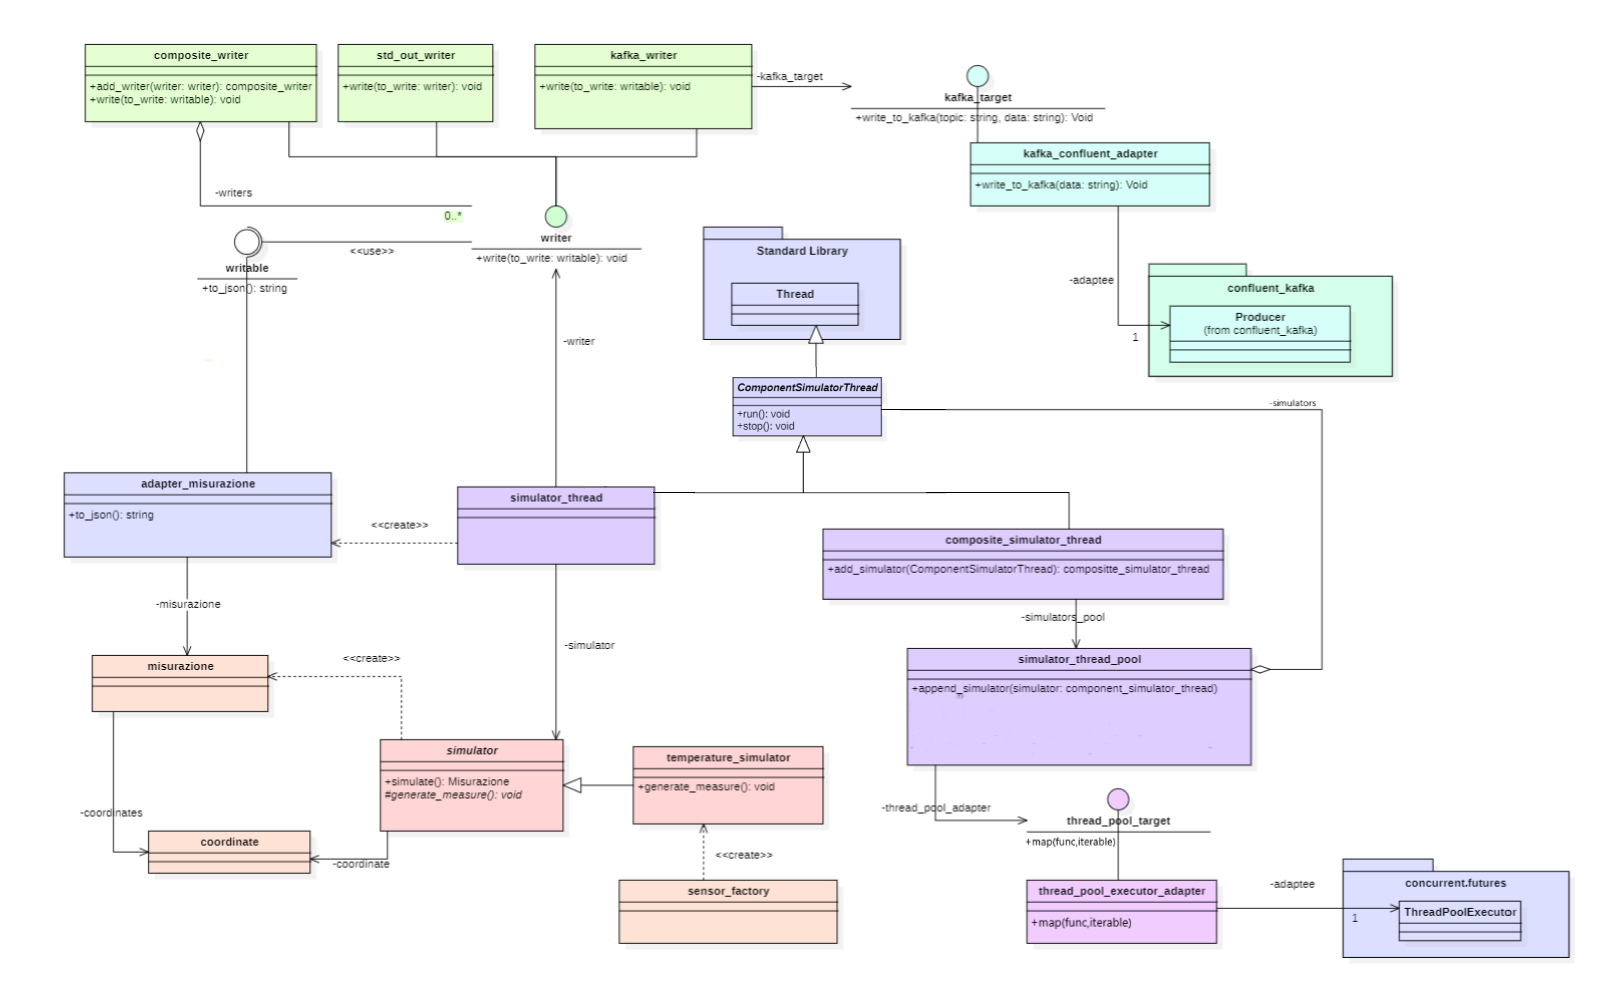
\includegraphics[width=1.1\textwidth]{../Images/SpecificaTecnica/progettazioneCompSimulatori.PNG}
    \caption{Panoramica progettazione simulatori sensori UML - InnovaCity}
    \label{fig: panor_sim}
\end{figure}
L'immagina vuole mostrare sinteticamente la struttura dei moduli \textit{Simulatori}, \textit{Writers} e \textit{Threading/Scheduling} e le relazioni tra le classi principali di questi moduli. In particolare, si evidenzia la presenza del pattern \textit{Composite} per la gestione di più servizi di scrittura e di più thread di esecuzione, il pattern \textit{Strategy} per la scrittura su diversi servizi e il pattern \textit{Object Adapter} per adattare le ThreadPool di Python e gli oggetti Misurazione ai writer. 
Viene riportato solo il sensore di temperatura come implementazione concreta di \textit{simulator} in quanto le altre implementazioni sono analoghe nel loro dominio.
\subsection{Kafka}
\subsubsection{Kafka topic}
I topic in \textit{Kafka}\textsubscript{\textit{G}} possono essere considerati come le tabelle di un \textit{database}\textsubscript{\textit{G}}, utili per separare logicamente diversi tipi di messaggi o eventi che vengono inseriti nel \textit{sistema}\textsubscript{\textit{G}}. Noi li utilizziamo per separare le diverse misurazioni dei sensori, quindi per ogni tipo di \textit{sensore}\textsubscript{\textit{G}} è presente un topic dedicato. Ciò ci consente di creare all'interno di \textit{ClickHouse}\textsubscript{\textit{G}} delle "tabelle consumatrici" che acquisiscono automaticamente i dati. Questo è possibile grazie alla separazione logica dei topic, che garantisce che tutti i messaggi all'interno di ciascun topic abbiano lo stesso formato.
\subsubsection{Formato messaggi} \label{sec:formatoMessaggi}
La struttura di un messaggio contenente le informazioni della misurazione è la seguente in formato Json e rispetta il contratto definito nello Schema Registry, vedi sez.\ref{sec:schema_registry}, in particolare \ref{sec:schema_registry_sez_schema}:
\begin{lstlisting}[style=code]
    {
      "timestamp": "AAAA-MM-DD HH:MM:SS.sss", 
      "value": "Valore della misurazione",  
      "type": "Tipologia Simulatore",
      "latitude": "Latitudine",
      "longitude": "Longitudine",
      "ID_sensore": "\textit{ID}\textsubscript{\textit{G}} \textit{sensore}\textsubscript{\textit{G}}",
      "cella": "Partizione della citt\`{a} dove \`{e} presente il sensore" 
     }
\end{lstlisting}
Mentre la struttura di un messaggio contenente le informazioni di una misurazione del punteggio di salute è la seguente in formato Json:
\begin{lstlisting}[style=code]
    {
      "timestamp": "AAAA-MM-DD HH:MM:SS.sss", 
      "value": "Valore della misurazione",  
      "type": "Tipologia Simulatore",
      "cella": "Cella relativa al punteggio di salute"
    }
\end{lstlisting}


Sebbene le misurazioni vengano divise in topic diversi a seconda della tipoligia di \textit{sensore}\textsubscript{\textit{G}} che ha effettuato la misurazione si è comunque deciso di inviare e salvare il campo della tipoligia di misurazione per i seguenti motivi:
\begin{itemize}
    \item \textbf{Backup e ripristino dei dati:} Se per qualche motivo si dovesse perdere la struttura dei topic o occorre ripristinare i dati in un altro \textit{sistema}\textsubscript{\textit{G}}, il campo type può aiutare a identificare il tipo di \textit{sensore}\textsubscript{\textit{G}} che ha effettuato la misurazione, anche se i dati sono stati conservati insieme in un unico topic.
    \item \textbf{Flessibilità futura:} 
    \begin{itemize}
        \item Potrebbero sorgere esigenze future che richiedono l'analisi dei dati provenienti da diversi tipi di sensori all'interno dello stesso topic. In questo caso, il campo type sarebbe utile per distinguere le misurazioni provenienti da sensori diversi;
        \item includere il campo type potrebbe essere particolarmente utile se si prevede di supportare diverse unità di misura per una stessa tipologia di \textit{sensore}\textsubscript{\textit{G}} in futuro. Ad esempio, potrebbe essere necessario gestire misurazioni di temperatura in gradi Celsius, Fahrenheit o Kelvin. In tal caso, includendo il campo type, si può associare ad ogni misurazione l'unità di misura corretta.
    \end{itemize}
\end{itemize}
    

\subsubsection{Kafka patterns}
\paragraph{Pattern di Pub/Sub}
\begin{itemize}
    \item \textbf{Descrizione:} Il \textit{pattern}\textsubscript{\textit{G}} Pub/Sub (Publish/Subscribe) permette ai producer di inviare messaggi a topic e ai consumer di ricevere messaggi da tali topic.
    \item \textbf{Funzione in Kafka:} Decoupling tra producer e consumer, favorendo la scalabilità e l'asincronia.
    \item \textbf{Esempio:} Un \textit{sensore}\textsubscript{\textit{G}} invia dati a \textit{Kafka}\textsubscript{\textit{G}} come producer. I dati vengono pubblicati su un topic specifico, e più consumer, come un'applicazione di analisi in tempo reale e un \textit{sistema}\textsubscript{\textit{G}} di archiviazione, si iscrivono al topic.
\end{itemize}

\paragraph{Partizionamento}
\begin{itemize}
    \item \textbf{Descrizione:} Distribuisce i messaggi su più partizioni all'interno di un topic per migliorare la scalabilità e le prestazioni.
    \item \textbf{Funzione in Kafka:} Permette di distribuire il carico di lavoro su più \textit{broker}\textsubscript{\textit{G}} e di aumentare la resilienza ai guasti.
    \item \textbf{Esempio:} I dati di un \textit{sensore}\textsubscript{\textit{G}} possono essere partizionati in base al tipo di \textit{sensore}\textsubscript{\textit{G}} o alla posizione geografica.
\end{itemize}

\paragraph{Replicazione}
\begin{itemize}
    \item \textbf{Descrizione:} Duplica i dati su più \textit{broker}\textsubscript{\textit{G}} per garantire la disponibilità e la tolleranza ai guasti.
    \item \textbf{Funzione in Kafka:} I messaggi vengono replicati su un numero configurabile di \textit{broker}\textsubscript{\textit{G}} per massimizzare la ridondanza.
    \item \textbf{Esempio:} Se un \textit{broker}\textsubscript{\textit{G}} fallisce, i dati sono ancora disponibili su altri \textit{broker}\textsubscript{\textit{G}}.
\end{itemize}



\paragraph{Leader Election}
\begin{itemize}
    \item \textbf{Descrizione:} Algoritmo per eleggere un leader per ogni partizione, responsabile dell'ordinamento e della replica dei messaggi.
    \item \textbf{Funzione in Kafka:} Garantisce la coerenza dei dati e la gestione efficiente delle partizioni.
    \item \textbf{Esempio:} Un leader viene eletto per ogni partizione del topic, garantendo che solo un \textit{broker}\textsubscript{\textit{G}} riceva e replichi i messaggi per quella partizione.
\end{itemize}


\paragraph{Log Compaction}
\begin{itemize}
    \item \textbf{Descrizione:} Rimuove i messaggi obsoleti da un topic per ottimizzare l'utilizzo dello \textit{storage}\textsubscript{\textit{G}}.
    \item \textbf{Funzione in Kafka:} Le vecchie versioni dei messaggi vengono eliminate dopo un periodo di tempo configurabile.
    \item \textbf{Esempio:} I messaggi di \textit{sensore}\textsubscript{\textit{G}} con valori vecchi possono essere compattati per risparmiare spazio di archiviazione.
\end{itemize}

\paragraph{Altri Pattern}
Oltre a quelli sopra elencati, \textit{Kafka}\textsubscript{\textit{G}} implementa altri \textit{pattern}\textsubscript{\textit{G}} come:
\begin{itemize}
    \item \textbf{Consumer Group}: Raggruppamento di consumer che collaborano per ricevere messaggi da un topic.
    \item \textbf{Coordinated Commit}: Meccanismo per garantire che tutti i consumer in un gruppo ricevano correttamente tutti i messaggi di una partizione.
    \item \textbf{Rate Limiting}: Controllo del numero di messaggi che possono essere inviati o ricevuti da un topic in un determinato intervallo di tempo.
    \item \textbf{Dead Letter Queue (DLQ)}: Coda speciale dove vengono inviati i messaggi che non possono essere elaborati correttamente.
    \item \textbf{Monitoring \& Metrics}: Fornisce un'ampia gamma di metriche per monitorare le prestazioni e l'utilizzo del \textit{sistema}\textsubscript{\textit{G}}.
\end{itemize}

\paragraph{Conclusione}
L'utilizzo di questi design \textit{pattern}\textsubscript{\textit{G}} rende \textit{Kafka}\textsubscript{\textit{G}} una \textit{piattaforma}\textsubscript{\textit{G}} di messaggistica robusta, scalabile e affidabile per una varietà di casi d'uso. L'implementazione di questi \textit{pattern}\textsubscript{\textit{G}} permette di ottenere un'\textit{architettura}\textsubscript{\textit{G}} efficiente e performante per l'elaborazione dati in streaming.
\subsection{Schema Registry} \label{sec:schema_registry}
\paragraph{Documentazione} \href{https://docs.confluent.io/platform/current/schema-registry/index.html}{https://docs.confluent.io/platform/current/schema-registry/index.html} (Consultato 25/03/2024)


Schema Registry fornisce un repository centralizzato per la gestione e la convalida degli schemi relativi ai dati dei messaggi degli argomenti, nonché per la serializzazione e la deserializzazione dei dati sulla rete. I produttori e i consumatori degli argomenti Kafka possono sfruttare gli schemi per garantire la coerenza e la compatibilità dei dati mentre questi ultimi si evolvono nel tempo. Il Schema Registry rappresenta un elemento chiave per la governance dei dati, poiché contribuisce ad assicurare la qualità dei dati, la conformità agli standard, la tracciabilità dell'origine dei dati, le capacità di audit, la collaborazione tra team, protocolli di sviluppo delle applicazioni efficienti e le prestazioni del sistema.


\begin{figure}[H]
    \centering
    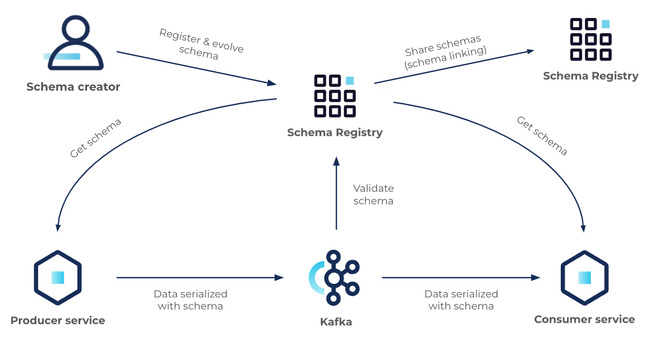
\includegraphics[width=0.9\textwidth]{../Images/SpecificaTecnica/schemaRegistry.jpg}
    \caption{Schema Registry Overview - Confluent Documentation}
    \label{fig:schemaReg}
  \end{figure}
La convalida del formato dei messaggi è un passo fondamentale per garantire l'integrità e l'affidabilità dei dati in un sistema di messaggistica come Apache Kafka. Schema Registry offre un potente strumento per la convalida dei messaggi in Kafka, fornendo diversi vantaggi:
\begin{enumerate}
    \item \textbf{Convalida dei messaggi:} Schema Registry convalida i messaggi in base allo schema registrato per il topic. I messaggi non validi vengono scartati.
    \item \textbf{Maggiore affidabilità:} La convalida dei messaggi aiuta a prevenire errori e a garantire che i dati siano conformi allo schema definito. Questo riduce il rischio di corruzione dei dati e di errori di elaborazione nei sistemi a valle.
    \item \textbf{Interoperabilità:} Schema Registry facilita la comunicazione tra diversi sistemi che producono e consumano messaggi Kafka. Definendo un formato comune per i messaggi, i sistemi possono interoperare senza problemi, anche se sono sviluppati in linguaggi di programmazione diversi o utilizzano librerie client differenti.
    \item \textbf{Evolutività:} Schema Registry permette di evolvere gli schemi dei messaggi nel tempo in modo compatibile. Ciò significa che è possibile aggiungere nuovi campi o modificare la struttura dei messaggi senza interrompere i sistemi esistenti.
    \item \textbf{Migliore debug:} La convalida dei messaggi fornisce informazioni utili in caso di errori, facilitando l'identificazione del problema e la sua risoluzione.
    \item \textbf{Sicurezza:} La convalida dei messaggi può essere utilizzata per proteggere il sistema da messaggi malformati o dannosi.
    
\end{enumerate}

Come funziona la convalida del formato dei messaggi con Schema Registry:
\begin{itemize}
    \item \textbf{Definizione dello schema:} Vengono definiti gli schemi per i messaggi Kafka utilizzando il formato JSON Schema e registrati in Schema Registry.
    \item \textbf{Produzione dei messaggi:} I producer Kafka inviano messaggi conformi allo schema definito. I messaggi possono essere inviati in topic specifici.
    \item \textbf{Convalida dei messaggi:} Schema Registry convalida i messaggi in base allo schema registrato per il topic. I messaggi non validi vengono scartati.
    \item \textbf{Consumo dei messaggi:} I consumer Kafka ricevono solo messaggi validi. I messaggi possono essere elaborati in modo affidabile dai sistemi a valle.
\end{itemize}

\subsubsection{Schema dei messaggi}\label{sec:schema_registry_sez_schema}
I messaggi nei topic dedicati allo streaming delle misurazioni dei sensori devono essere nel seguente formato per superare la convalida definita da contratto nello Schema Registry.
\paragraph{Misurazioni dei senori}
\begin{lstlisting}[style=code]
    {
        "type": "record",
        "name": "Misurazione",
        "fields": [
          {
            "name": "timestamp",
            "type": "string"
          },
          {
            "name": "value",
            "type": "float"
          },
          {
            "name": "type",
            "type": "string"
          },
          {
            "name": "latitude",
            "type": "float"
          },
          {
            "name": "longitude",
            "type": "float"
          },
          {
            "name": "ID_sensore",
            "type": "string"
          },
          {
            "name": "cella",
            "type": "string"
          }
        ]
      }
\end{lstlisting}


\paragraph{Misurazioni del punteggio di salute}
I messaggi nel topic dedicato allo streaming delle misurazioni dei punteggi di salute devono essere nel seguente formato per superare la convalida definita da contratto nello Schema Registry.
\begin{lstlisting}[style=code]
    {
        "type": "record",
        "name": "MisurazioneSalute",
        "fields": [
          {
            "name": "timestamp",
            "type": "string"
          },
          {
            "name": "value",
            "type": "float"
          },
          {
            "name": "type",
            "type": "string"
          },
          {
            "name": "cella",
            "type": "string"
          }
        ]
      }
    \end{lstlisting}

\subsection{Faust - Processing Layer} \label{sec:faust}
\subsubsection{Introduzione}
\paragraph*{Premessa}

Per soddisfare il requisito opzionale del calcolo del punteggio di salute, si è scelto di utilizzare Faust, una libreria Python ispirata al modello di Kafka Streams. Faust facilita l'elaborazione di flussi di dati distribuiti in tempo reale, rendendola ideale per questo caso d'uso.
Offre un'interfaccia di alto livello che astrae le complessità di Kafka, rendendo la raccolta dati semplice e intuitiva.
Inolltre Faust è progettato per essere scalabile e può essere utilizzato per gestire grandi volumi di dati.

\paragraph*{Calcolo del Punteggio}
Il punteggio di salute rappresenta un indicatore sintetico del benessere generale di una città, misurandolo in base a diversi aspetti chiave. In questo caso, le tre tipologie di misurazioni considerate sono:
\begin{itemize}
    \item Temperatura;
    \item Umidità;
    \item Livello di polveri sottili (PM10).
\end{itemize}

Il calcolo del punteggio avviene in due fasi:
\begin{enumerate}
    \item \textbf{Incrementi}: 
    \begin{itemize}
        \item A intervalli regolari, si calcolano incrementi al punteggio di salute basandosi sulle misurazioni acquisite nell'intervallo precedente.
        \item Ciascuna tipologia di misurazione ha un suo algoritmo di calcolo dell'incremento, basato su soglie predefinite di benessere.
    \end{itemize}
    \item \textbf{Punteggio Finale}:
    \begin{itemize}
        \item Il punteggio di salute finale si ottiene sommando gli incrementi calcolati per le tre tipologie di misurazioni.
        \item Punteggi più alti indicano un minore stato di benessere, con la necessità di interventi per migliorare la qualità della vita.
    \end{itemize}
\end{enumerate}


\subsubsection{Componenti Faust \& Processing Layer}
\begin{itemize}
    \item \textbf{Applicazione Faust:}
    \begin{lstlisting}[style=code]
        faust.App(<nome_app>, broker=<broker_kafka>)
    \end{lstlisting} 
    \begin{itemize}
        \item Un'applicazione Faust è un programma Python che elabora flussi di dati in tempo reale da Kafka.
        \item \textbf{nome\_app}: Identifica l'applicazione.
        \item \textbf{broker\_kafka}: Indirizzo del broker Kafka (hostname:porta).
    \end{itemize}
    \item \textbf{Topic:}
    \begin{lstlisting}[style=code]
        app.topic(<nome_topic>, value_type=<tipo_dato>)
    \end{lstlisting}  
    \begin{itemize}
        \item \textbf{nome\_topic}: Nome del topic Kafka.
        \item \textbf{tipo\_dato:} Classe che rappresenta il tipo di dato del topic (es. FaustMeasurement).
        \item Nel caso si voglia aggiungere altri topic da cui consumare dati basterà aggiungerne prima del parametro value\_type.
    \end{itemize}
    \item \textbf{Tipo di dato atteso:}
     \begin{lstlisting}[style=code]
        class FaustMeasurement(faust.Record)
    \end{lstlisting}  
    \begin{itemize}
        \item È una classe che eredita da \textbf{faust.Record}.
        \item \textbf{faust.Record} è una classe fornita dalla libreria Faust che semplifica la definizione di record per la rappresentazione dei dati in streaming.
        \item Rappresenta una singola misurazione proveniente da un sensore. Viene usata nella applicazione Faust per definire il tipo di dati atteso nei topic Kafka.
    \end{itemize}
    \item \textbf{Modello per il calcolo del punteggio di salute:}:
    \begin{itemize}
        \item \textbf{Processore di misurazioni}: 
        Tramite il pattern \textit{Object Adapter} e l'interfaccia \textit{Processor} l'app faust invia le misurazioni ottenute dai topic al modello per il calcolo del punteggio di salute che verrà adattato come \textit{Processor.}
    \end{itemize}
    \item \textbf{Agente di elaborazione}: 
    \begin{lstlisting}[style=code]
        @app.agent(<topic>).
    \end{lstlisting}  
    \begin{itemize}
        \item Funzioni asincrone che elaborano i dati dai topic;
        \item Ricevono un iteratore di oggetti del tipo specificato per il topic;
        \item Eseguono l'elaborazione desiderata su ogni misurazione.
    \end{itemize}
    \item \textbf{Interfaccia Processor}:
    \begin{itemize}
        \item Per l'incapsulamento di logiche di elaborazione.
        \item Utilizzata dagli agenti di elaborazione per inviare le misurazioni al modello per il calcolo del punteggio di salute.
    \end{itemize}
    \item \textbf{Task aggiuntivo} (opzionale): 
    \begin{lstlisting}[style=code]
    @app.task()
        \end{lstlisting}  
    \begin{itemize}
        \item Definisce una funzione eseguita una sola volta all'avvio dell'applicazione.
    \end{itemize}
\end{itemize}

\subsubsection{Modello per il calcolo del punteggio di salute}
\begin{figure}[H]
    \centering
    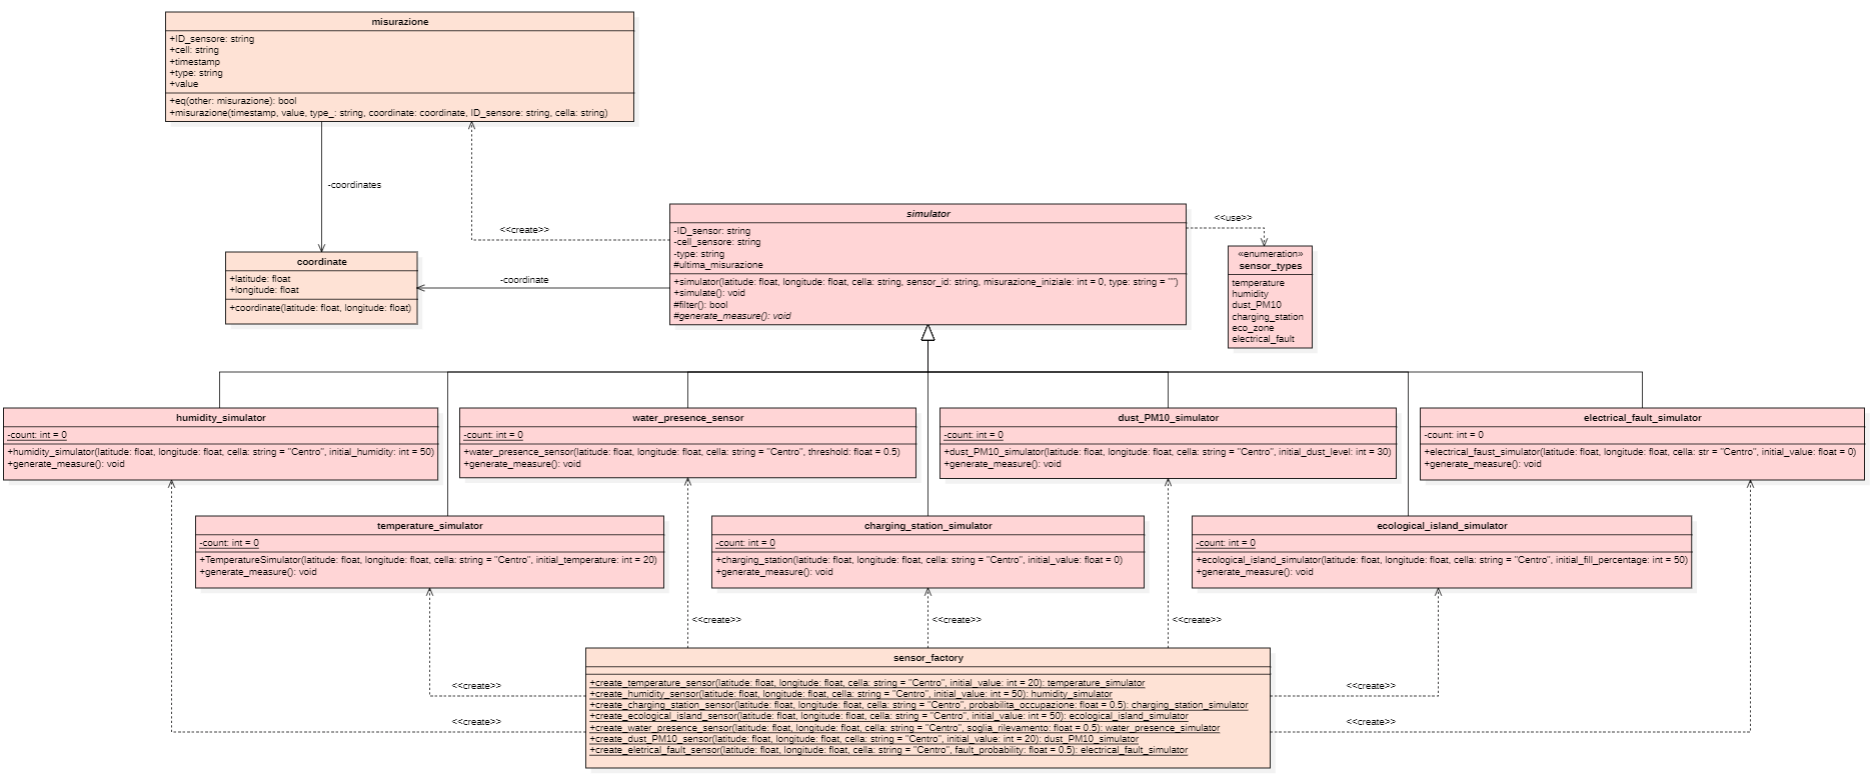
\includegraphics[width=1\textwidth]{../Images/SpecificaTecnica/simulatoriSensori.PNG}
    \caption{Modulo simulatori sensori - Innovacity}
    \label{fig: fddf}
\end{figure}

Il processo per il calcolo del punteggio di salute riceve le letture dei sensori attraverso gli agenti di elaborazione dell'applicazione Faust, i quali sono in ascolto sui topic Kafka relativi alle misurazioni di temperatura, umidità e polveri sottili PM10. Ad intervalli regolari, il sistema calcola il punteggio di salute della città basandosi su tali misurazioni. Una volta effettuato il calcolo, il risultato è reso disponibile in un topic Kafka dedicato.
Il modello che racchiude la logica per il calcolo, richiamato a intervalli regolari, è quello attualmente preso in esame.

In sintesi, il modello:
\begin{itemize}
    \item Riceve le misurazioni di temperatura, umidità e polveri sottili dall'agente dell'app Faust.
    \item Riceve da un thread la richiesta ad intervalli regolari di calcolare i punteggi di salute per le celle della città con le misurazioni ottenute in tempo reale.
\end{itemize}

In accordo con l'architettura esagonale, la logica del modello è completamente disaccoppiata dai suoi utilizzatori, i quali interagiscono con il modello tramite specifiche classi adapter. Questo approccio promuove la separazione delle preoccupazioni e favorisce la modularità del sistema. Gli adapter fungono da ponte tra il modello e gli utilizzatori, consentendo una comunicazione fluida e senza dipendenze dirette. Così, eventuali cambiamenti nella logica del modello possono essere implementati senza influenzare gli utilizzatori, garantendo una maggiore flessibilità e manutenibilità del sistema nel suo complesso.

Il presente modulo è concepito per fornire la logica relativa al puro calcolo del punteggio di salute della città. Tale calcolo si basa su un modello che tiene conto delle misurazioni di temperatura, umidità e polveri sottili PM10. Il modello è stato progettato al fine di determinare un punteggio di salute per ciascuna cella della città in cui sono presenti misurazioni delle suddette tipologie.

\paragraph*{Design Pattern Strategy}

Il modello per il calcolo del punteggio di salute è stato ideato mediante l'utilizzo del design pattern Strategy. Tale pattern consente di definire una famiglia di algoritmi, di incapsularli e renderli intercambiabili. Ciò permette di variare l'algoritmo impiegato per il calcolo del punteggio di salute senza incidere sui processi di elaborazione dell'applicazione Faust o sugli altri componenti del sistema. In particolare, l'interfaccia \textit{HealthAlgorithm} stabilisce il contratto che deve essere rispettato da tutti gli algoritmi per il calcolo del punteggio di salute.


Inoltre, un'implementazione del pattern \textit{Strategy} è presente anche negli "Incrementatori". Questi, a partire dalle misurazioni fornite, restituiscono un incremento al punteggio di salute della città. Tale incremento è determinato in base a delle soglie predefinite di temperatura, umidità e polveri sottili PM10, le quali sono definite di default in \textit{health\_constants} ma possono essere impostate al momento della costruzione. In particolare, l'interfaccia \textit{Incrementer} specifica il contratto che deve essere rispettato da tutti gli incrementatori. Vengono implementati tre incrementatori, uno per il calcolo dell'incremento di temperatura, uno per l'umidità e uno per le polveri sottili PM10, come strategie del pattern.

\paragraph{Classi: metodi e attributi}
\begin{itemize}
    \item{\textbf{Interfaccia: \textit{HealthAlgorithm}}}
    \begin{itemize}
    \item \textbf{Metodi: }
    \begin{itemize}
        \item \textbf{generate\_new\_health\_score(): List[MisurazioneSalute] [abstractmethod]} - Un metodo astratto che deve essere implementato nelle sottoclassi. Questo metodo dovrebbe generare un nuovo punteggio di salute.
    \end{itemize}
    \item\textbf{Note}:
        \begin{itemize}
            \item L'interfaccia definisce il contratto per un algoritmo di salute. Le sottoclassi devono implementare il metodo \textit{generate\_new\_health\_score};
            \item Rappresenta la componente "Strategy" del pattern omonimo.
            \item Per rispettare il Single responsibility principle, noto anche come principio di coesione, è stata divisa dalla logica di buffering delle misurazioni presente nella classe astratta \textit{HealthProcessorBuffer} poiché l'utilizzatore \textit{HealthCalculatorThread} non utilizza i metodi per il buffering.
        \end{itemize}
    \end{itemize}
    \item\textbf{Classe astratta: \textit{HealthProcessorBuffer}}
    \begin{itemize}
    \item\textbf{Attributi}:
        \begin{itemize}
        \item \textbf{lista\_misurazioni:lista\_misurazioni [private]} - Una lista di oggetti Misurazione.
        \item \textbf{lock:threading.Lock [private]} - Un oggetto lock per gestire l'accesso concorrente alla lista di misurazioni.
    \end{itemize}
    \item \textbf{Metodi: }
    \begin{itemize}
        \item \textbf{add\_misurazione(timestamp, value, type\_, latitude, longitude, ID\_sensore, cella): None [public]} - Aggiunge una nuova misurazione alla lista di misurazioni.
        \item \textbf{clear\_list(): None [public]} - Svuota la lista di misurazioni.
    \end{itemize}
    \item\textbf{Note}:
        \begin{itemize}
               \item La classe astratta definisce un buffer di misurazioni per effettuare il processing su un set di misurazioni. Tale buffer contiene una lista di misurazioni e fornisce metodi per aggiungere misurazioni, ottenere la lista di misurazioni e svuotare la lista.
                \item La logica di buffering e quella dell'algoritmo per il calcolo del punteggio di salute vengono separate in due astrazioni per rispettare il principio di Single Responsibility. Gli utilizzatori di questa classe, i \textit{Processor}, sono interessati esclusivamente al metodo per l'invio del dato al buffer.
                \item La classe astratta definisce un'interfaccia per la comunicazione con gli utilizzatori esterni al modello.
        \end{itemize}
    \end{itemize}
    \item{\textbf{Classe: \textit{HealthCalculator}}}
    \begin{itemize}
    \item\textbf{Attributi}:
        \begin{itemize}
        \item \textbf{tmpInc:TemperatureIncrementer [private]} - Utilizzato per il calcolo dell'incremento di temperatura;
        \item \textbf{umdInc:HumidityIncrementer [private]}; - Utilizzato per il calcolo dell'incremento di umidità;
        \item \textbf{dstPm10Inc:DustPM10Incrementer [private]} - Utilizzato per il calcolo dell'incremento di PM10;
        \item \textbf{temperature\_measure\_type\_naming:string [private]} - Nomenclatura dei tipi di misurazione di temperatura.
        \item \textbf{humidity\_measure\_type\_naming:string [private]} - Nomenclatura dei tipi di misurazione di umidità.
        \item \textbf{ dtsPm10\_measure\_type\_naming:string [private]} - Nomenclatura dei tipi di misurazione di PM10.
        \item \textbf{ healthScore\_measure\_type\_naming:string [private]} - Nomenclatura dei tipi di misurazione di punteggio di salute.
        \item \textbf{lock [private]} - Un oggetto lock per gestire l'accesso concorrente.
    \end{itemize}
    \item \textbf{Metodi: }
    \begin{itemize}
        \item \textbf{generate\_new\_health\_score(): List[MisurazioneSalute] [public]} - Genera e restituisce una nuova lista di punteggi di salute, uno per ogni cella della città di cui sono state fornite misurazioni.
        \item \textbf{calcola\_incremento\_tmp(cella: str, lista\_misurazioni): int [private]} - Calcola e restituisce l'incremento della temperatura.
        \item \textbf{calcola\_incremento\_umd(cella: str, lista\_misurazioni): int [private]} - Calcola e restituisce l'incremento dell'umidità.
        \item \textbf{calcola\_incremento\_dstPm10(cella: str, lista\_misurazioni): int [private]} - Calcola e restituisce l'incremento della polvere PM10.
    \end{itemize}
    \item\textbf{Note}:
        \begin{itemize}
            \item La classe implementa l'interfaccia \textit{HealthAlgorithm} e la classe astratta \textit{HealthProcessorBuffer} per calcolare il punteggio di salute tramite la strategia concreta definita in \textit{generate\_new\_health\_score()} che genera una nuova lista di punteggi di salute.
            \item Questa classe rappresenta il vero cervello del calcolo del punteggio di salute in quanto utilizzatore di tutti gli incrementatori e delle misurazioni bufferizzate per creare una strategia di calcolo.
        \end{itemize}
    \end{itemize}
    \item\textbf{Classe: \textit{Misurazione}}
    \begin{itemize}
        \item   \textbf{Attributi}: 
    \begin{itemize}
        \item \textbf{timestamp:datetime [private]} - Timestamp della misurazione.
        \item \textbf{value:T [private]} - Valore della misurazione.
        \item \textbf{type:str [private]} - Tipo della misurazione.
        \item \textbf{coordinates:coordinate [private]} - Coordinate della misurazione.
        \item \textbf{ID\_sensore:str [private]} - ID del sensore che ha effettuato la misurazione.
        \item \textbf{cella:str [private]} - Cella in cui è stata effettuata la misurazione.
    \end{itemize}
    \item   \textbf{Metodi}: 
    \begin{itemize}
        \item \textbf{\_\_eq\_\_(other:Misurazione):bool [public]} - Ridefinizione dell'operatore di uguaglianza per confrontare due oggetti Misurazione.
    \end{itemize}
\end{itemize}
    \item\textbf{Classe: \textit{coordinate}}
    \begin{itemize}
        \item    \textbf{Attributi}: 
    \begin{itemize}
        \item \textbf{latitude:float [private]} - Latitudine della coordinata.
        \item \textbf{longitude:float [private]} - Longitudine della coordinata.
    \end{itemize}
    \item     \textbf{Metodi}: 
    \begin{itemize}
        \item \textbf{\_\_eq\_\_(other:coordinate):bool [public]} - Ridefinizione dell'operatore di uguaglianza per confrontare due oggetti Coordinate.
    \end{itemize}
\end{itemize}
\item\textbf{Classe: \textit{MisurazioneSalute}}
    \begin{itemize}
    \item\textbf{Attributi}:
        \begin{itemize}
        \item \textbf{timestamp:datetime [private]} - Il timestamp della misurazione di salute.
        \item \textbf{value:float [private]} - Il valore della misurazione di salute.
        \item \textbf{type:string [private]} - Il tipo della misurazione.
        \item \textbf{cella:string [private]} - La cella della misurazione di salute.
    \end{itemize}
    \item\textbf{Note}:
        \begin{itemize}
            \item La classe rappresenta una misurazione di salute. Contiene informazioni sul timestamp, il valore (ovvero il punteggio di salute calcolato), il tipo della misurazione e la cella relativa alla misurazione.
        \end{itemize}
    \end{itemize}
    \item\textbf{Classe: \textit{lista\_misurazioni}}
    \begin{itemize}
    \item\textbf{Attributi}:
        \begin{itemize}
        \item \textbf{list:List[Misurazione] [private]} - Una lista di oggetti Misurazione.
    \end{itemize}
    \item \textbf{Metodi: }
    \begin{itemize}
        \item \textbf{add\_misurazione(timestamp, value, type\_, latitude, longitude, ID\_sensore, cella): None [public]} - Aggiunge una nuova misurazione alla lista.
        \item \textbf{clear\_list(): None [public]} - Svuota la lista di misurazioni.
        \item \textbf{get\_list\_by\_cella\_and\_type(cella: str, tipo\_dato: str): List[Misurazione] [public]} - Restituisce una lista di misurazioni che corrispondono alla cella e al tipo di misurazione specificati (temperatura,umidità,ecc.).
        \item \textbf{get\_unique\_celle(): List[str] [public]} - Restituisce la lista di celle presenti nelle misurazioni senza ripetzioni.
    \end{itemize}
    \item\textbf{Note}:
        \begin{itemize}
            \item La classe rappresenta una lista di misurazioni. Fornisce metodi per aggiungere misurazioni, svuotare la lista, ottenere misurazioni per cella e tipo di misurazioni, e ottenere le celle di cui si hanno misurazioni.
        \end{itemize}
    \end{itemize}
    \item\textbf{Enumerazione: \textit{SensorTypes}}
        \begin{itemize}
            \item \textbf{Costanti}: 
            \begin{itemize}
                \item \textbf{TEMPERATURE:str [public]} - Rappresenta la nomenclatura dei sensore di temperatura.
                \item \textbf{HUMIDITY:str [public]} - Rappresenta la nomenclatura dei sensore di umidità.
                \item \textbf{DUST\_PM10:str [public]} - Rappresenta la nomenclatura dei sensore di "polvere PM10".
                \item \textbf{CHARGING\_STATION:str [public]} - Rappresenta la nomenclatura dei sensore di stato delle colonnine di ricarica.
                \item \textbf{ECOLOGICAL\_ISLAND:str [public]} - Rappresenta la nomenclatura dei sensore di stato riempimento isole ecologica.
                \item \textbf{WATER\_PRESENCE:str [public]} - Rappresenta la nomenclatura dei sensore di presenza d'acqua.
                \item \textbf{ELECTRICAL\_FAULT:str [public]} - Rappresenta la nomenclatura dei sensore di guasti elettrici.
            \end{itemize}

            \item \textbf{Note}:
            \begin{itemize}
                \item L'enumerazione viene utilizzata per centralizzare la gestione della nomenclatura dei tipi di sensori che verrà salvata nelle misurazioni.
            \end{itemize}
        \end{itemize}
\item \textbf{Interfaccia: \textit{Incrementer}}
    \begin{itemize}
    \item \textbf{Metodi: }
    \begin{itemize}
        \item \textbf{get\_incrementation(misurazioni: List[Misurazione]): int [abstractmethod]} - Un metodo astratto che deve essere implementato nelle sottoclassi. Questo metodo calcola e restituire un incremento basato sulla lista di misurazioni fornita.
    \end{itemize}
    \item\textbf{Note}:
        \begin{itemize}
            \item L'interfaccia definisce il contratto per un incrementatore. Le sottoclassi devono implementare il metodo \textit{get\_incrementation()}.
            \item Rappresenta la componente "Strategy" del pattern omonimo.
        \end{itemize}
    \end{itemize}
    \item \textbf{Classe: \textit{TemperatureIncrementer}}
    \begin{itemize}
    \item \textbf{Attributi}:
        \begin{itemize}
        \item \textbf{upper\_health\_soglia:int [private]} - La soglia superiore di benessere per la temperatura;
        \item \textbf{under\_health\_soglia:int [private]} - La soglia inferiore di benessere per la temperatura.
    \end{itemize}
    \item \textbf{Metodi: }
    \begin{itemize}
        \item \textbf{get\_incrementation(misurazioni: List[Misurazione]): int [public]} - Calcola e restituisce un incremento basato sulle sole misurazioni di temperatura della lista fornita.
    \end{itemize}
    \item\textbf{Note}:
        \begin{itemize}
            \item La classe implementa l'interfaccia \textit{Incrementer};
            \item I valori di default per le soglie vengono presi dall'enumerazione \textit{HealthConstant} altrimenti sono impostabili alla costruzione.
            \item Rappresenta una strategia concreta del pattern \textit{Strategy} per il calcolo dell'incremento di temperatura.
        \end{itemize}
    \end{itemize}
    \item{\textbf{Classe: \textit{HumidityIncrementer}}}
    \begin{itemize}
    \item\textbf{Attributi}:
        \begin{itemize}
        \item \textbf{upper\_health\_soglia:int [private]} - La soglia superiore di benessere per l'umidità;
        \item \textbf{under\_health\_soglia:int [private]} - La soglia inferiore di benessere per l'umidità.
    \end{itemize}
    \item \textbf{Metodi: }
    \begin{itemize}
        \item \textbf{get\_incrementation(misurazioni: List[Misurazione]): int [public]} - Calcola e restituisce un incremento basato sulle sole misurazioni di umidità della lista fornita.
    \end{itemize}
    \item\textbf{Note}:
        \begin{itemize}
            \item La classe implementa l'interfaccia \textit{Incrementer};
            \item I valori di default per le soglie vengono presi dall'enumerazione \textit{HealthConstant} altrimenti sono impostabili alla costruzione.
            \item Rappresenta una strategia concreta del pattern \textit{Strategy} per il calcolo dell'incremento di umidità.
        \end{itemize}
    \end{itemize}\item{\textbf{Classe: \textit{DustPM10Incrementer}}}
    \begin{itemize}
    \item \textbf{Metodi: } 
    \begin{itemize}
        \item \textbf{get\_incrementation(misurazioni: List[Misurazione]): int [public]} - Calcola e restituisce un incremento basato sulle sole misurazioni di polveri sottili della lista fornita.
    \end{itemize}
    \item\textbf{Note}:
        \begin{itemize}
            \item La classe implementa l'interfaccia \textit{Incrementer};
            \item Rappresenta una strategia concreta del pattern \textit{Strategy} per il calcolo dell'incremento di polveri sottili PM10.
            \item A differenza degli altri \textit{Incrementer}, \textit{DustPM10Incrementer} non definisce soglie di benessere in quanto è scontato che il valore ottimale di inquinamento è zero.
        \end{itemize}
    \end{itemize}

\end{itemize}

\subsubsection{Modulo Writer}
Il modulo Writer è lo stesso di quello descritto in \ref*{sec:writersModule} e viene nella sua totalità riutilizzato per la scrittura dei punteggi di salute calcolati.
Non viene riportata la strategia di scrittura su di una lista poichè non ne è stato ritenuto necessario l'utilizzo.

\paragraph*{Classi: metodi e attributi}
Tutte le informazioni sono già state esposte in: \ref*{sec:writersModule}.

\subsubsection{Modulo Threading/Scheduling}
\begin{figure}[H]
    \centering
    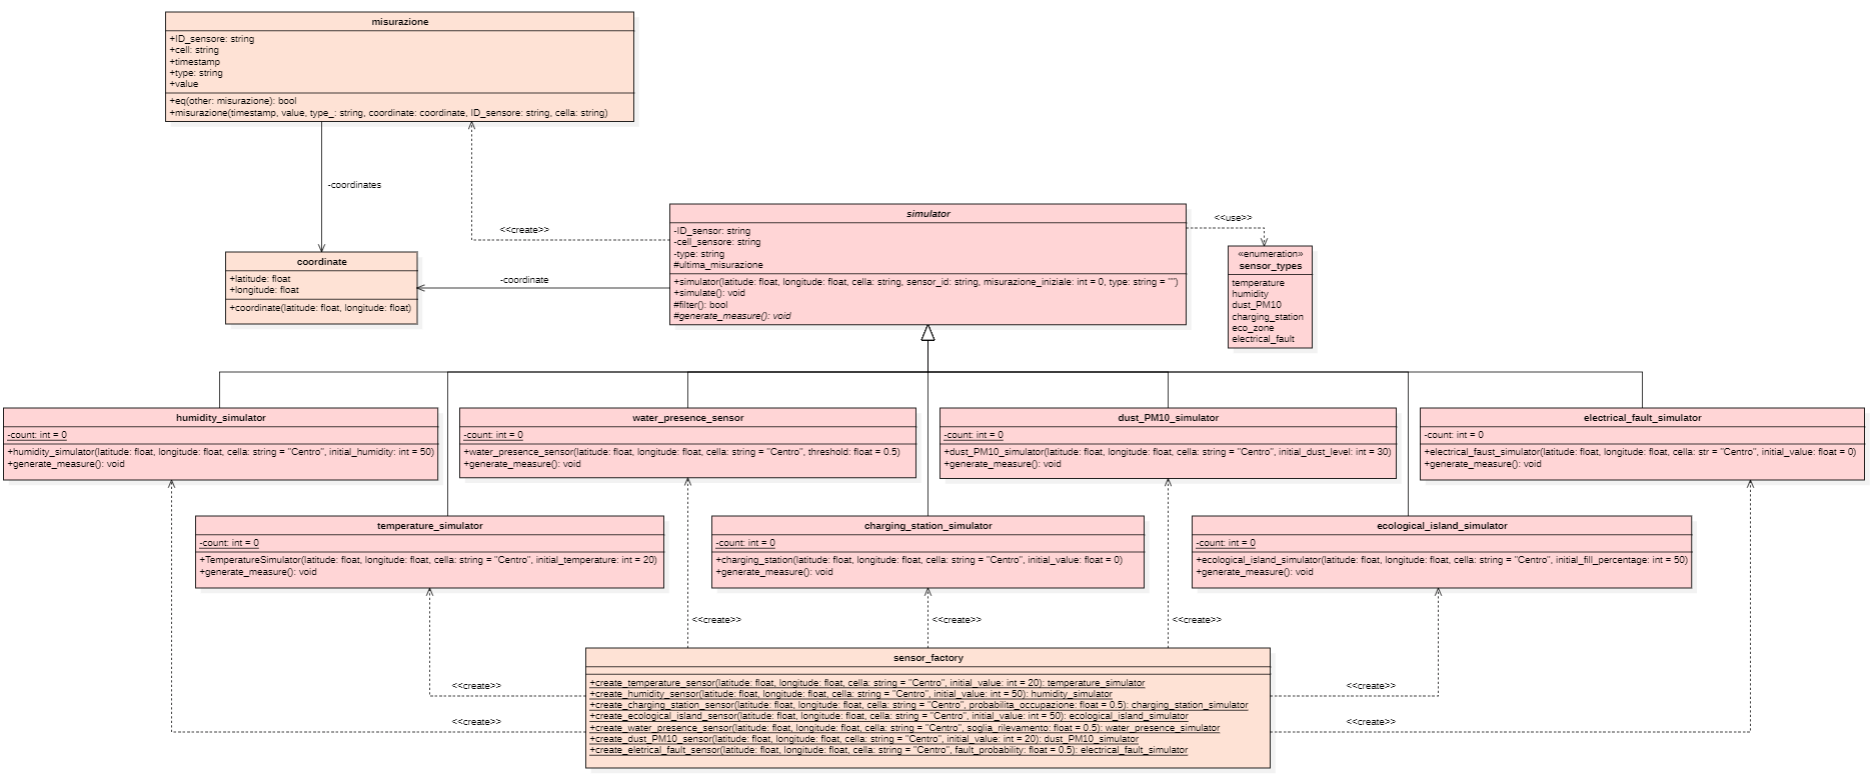
\includegraphics[width=1\textwidth]{../Images/SpecificaTecnica/simulatoriSensori.PNG}
    \caption{Modulo simulatori sensori - Innovacity}
    \label{fig: fddf}
\end{figure}

Questo modulo si occupa di integrare la logica di Scheduling e Threading per il calcolo periodico del punteggio di salute della città e quella di scrittura/invio di \textit{Writable}. In particolare, fornisce un'implementazione di un thread che, a intervalli regolari, richiama il calcolo del punteggio di salute della città. Successivamente, utilizzando il modulo "Writer", adatta le misurazioni di salute ottenute all'interfaccia per renderle un oggetto che implementa \textit{Writable}. Pertanto, questo modulo è utilizzatore del modello per il calcolo del punteggio di salute e del modulo di Writer.
In sintesi, il modulo:
    \begin{enumerate}
        \item Richiama l'algoritmo per calcolo del punteggio di salute della città a intervalli regolari;
        \item Scrive il risultato ottenuto sul topic Kafka dedicato.
    \end{enumerate}

\paragraph*{Dependecy Inversion principle}
Il modulo di scheduling e threading dipende dall'astrazione dell'interfaccia del modello per il calcolo del punteggio di salute e del modulo di Writer, invece di dipendere direttamente dalle implementazioni concrete di questi moduli. Ciò consente una maggiore flessibilità e facilità di manutenzione, poiché il modulo di scheduling e threading non è vincolato a implementazioni specifiche, ma può essere facilmente adattato per utilizzare diverse implementazioni che soddisfano lo stesso contratto.

In sostanza, seguendo il principio di Inversione delle Dipendenze, il modulo di scheduling e threading si concentra sull'utilizzo di interfacce o astrazioni, piuttosto che sulle implementazioni concrete, rendendo il sistema più modulare, scalabile e facilmente estendibile.

\paragraph*{Classi: metodi e attributi}
\begin{itemize}
    \item{\textbf{Classe: \textit{HealthCalculatorThread}}}
    \begin{itemize}
    \item\textbf{Attributi}:
        \begin{itemize}
        \item \textbf{healthCalculator: HealthAlgorithm [private]} - Un implementatazione dell'interfaccia \textit{HealthAlgorithm}, ovvero una strategia per il calcolo del punteggio.
        \item \textbf{frequency: float [private]} - La frequenza con cui il thread genera nuovi punteggi di salute.
        \item \textbf{is\_running: bool [private]} - Un flag che indica se il thread è in esecuzione.
        \item \textbf{data\_to\_generate: int [private]} - Il numero di misurazioni di salute da generare.
        \item \textbf{writers: Writer [private]} - Un oggetto della classe Writer. (Singolo scrittore o albero, Composite pattern)
    \end{itemize}
    \item \textbf{Metodi: }
    \begin{itemize}
        \item \textbf{run(): None [public]} - Esegue il thread, generando nuovi punteggi di salute a una certa frequenza.
        \item \textbf{stop(): None [public]} - Ferma l'esecuzione del thread.
    \end{itemize}
    \item\textbf{Note}:
        \begin{itemize}
            \item La classe estende la classe \textit{threading.Thread}.
            \item Se \textit{data\_to\_generate} è < 0 genera misurazioni di salute finchè il thread non viene interroto dall'esterno.
            \item   Grazie al pattern \textit{Strategy} è possibile cambiare agevolmente l'algoritmo volto al calcolo del punteggio di salute della città.
        \end{itemize}
    \end{itemize}
\end{itemize}

\subsubsection{Modulo Processing}
Per garantire un'interfaccia uniforme per i metodi di elaborazione dei dati provenienti da Kafka tramite Faust e per stabilire un canale di comunicazione con il modello per il calcolo del punteggio di salute, viene sviluppato il modulo di Processing. Questo modulo offre l'interfaccia target denominata \textit{Processor}, e un adapter a \textit{Processor} per l'invio delle misurazioni al modello per il calcolo del punteggio di salute, denominato \textit{HealthModelProcessorAdapter}.

\paragraph*{Design Pattern Object Adapter}
Nel contesto dell'applicazione Faust, all'interno del ruolo svolto dagli agenti, ogni volta che una misurazione viene ricevuta, viene invocato il metodo \textit{process\_measure()} dell'implementazione dell'interfaccia \textit{Processor}, denominata \textit{HealthModelProcessorAdapter}. In particolare, \textit{HealthModelProcessorAdapter} adatta la classe astratta \textit{HealthModelBuffer}, che rappresenta un buffer di misurazioni utilizzato per eseguire il calcolo periodico del punteggio di salute della città, all'interfaccia \textit{Processor}.

Questo pattern consente di incapsulare le logiche di elaborazione e di rendere il modello indipendente dall'implementazione specifica dell'applicazione Faust. Allo stesso tempo, facilita la sostituzione dell'operazione di elaborazione eseguita su ogni misurazione dagli agenti grazie al contratto dell'interfaccia \textit{Processor}.
\paragraph*{Classi: metodi e attributi}
\begin{itemize}
    \item{\textbf{Interfaccia: \textit{Processor}}}
    \begin{itemize}
    \item\textbf{Metodi: }
    \begin{itemize}
        \item \textbf{process(misurazione: FaustMeasurement): None [public, abstract]} - Un metodo astratto che deve essere implementato nelle sottoclassi. Questo metodo elabora una misurazione.
    \end{itemize}
    \item\textbf{Note}:
        \begin{itemize}
            \item  Le sottoclassi devono implementare il metodo astratto \textit{process()} definendo la propria operazione da effettuare su ogni misurazione ricevuta dai topic di iscrizione.
            \item Rappresenta la componente "Target" del pattern \textit{Object Adapter}.
            \item L'interfaccia è stata progettata per garantire un'interfaccia uniforme per i metodi di elaborazione dei dati provenienti da Kafka tramite Faust.
            \item Rappresenta un contratto per l'elaborazione di misurazioni.
            \item Gli agenti in ascolto sul topic utilizzeranno un implementatazione di \textit{Processor} per effettuare l'elaborazione delle misurazioni ottenute.
        \end{itemize}
    \end{itemize}
    \item{\textbf{Classe: \textit{FaustMeasurement}}}
    \begin{itemize}
    \item\textbf{Attributi}:
        \begin{itemize}
        \item \textbf{timestamp: str} - Il timestamp della misurazione.
        \item \textbf{value: float} - Il valore della misurazione.
        \item \textbf{type: str} - Il tipo della misurazione.
        \item \textbf{latitude: float} - La latitudine della misurazione.
        \item \textbf{longitude: float} - La longitudine della misurazione.
        \item \textbf{ID\_sensore: str} - L'ID del sensore che ha effettuato la misurazione.
        \item \textbf{cella: str} - La cella della misurazione.
    \end{itemize}
    \item\textbf{Note}:
        \begin{itemize}
            \item La classe \textit{FaustMeasurement} definita utilizzando \textit{faust.Record} rappresenta un singolo record di misurazione proveniente da un sensore in un'applicazione Faust basata su Python
            \item Faust si occupa automaticamente della conversione dei dati in formato JSON in base agli attributi definiti, facilitando la trasmissione e la ricezione dei dati nei topic Kafka.
            \item È possibile definire la validazione dei dati in ingresso per garantire l'integrità e la coerenza delle misurazioni.
            \item \textbf{In sintesi}:
            Questa classe viene utilizzata in un'applicazione Faust per definire il tipo di dati atteso nei topic Kafka. I dati provenienti dai sensori, contenenti timestamp, valore, tipo, coordinate geografiche, identificativo del sensore e eventuale cella di appartenenza, verranno convertiti in oggetti di tipo FaustMeasurement prima di essere elaborati dall'applicazione.
        \end{itemize}
    \end{itemize}
    \item{\textbf{Classe: \textit{HealthModelProcessorAdapter}}}
    \begin{itemize}
    \item\textbf{Attributi}:
        \begin{itemize}
        \item \textbf{healthCalculator: HealthProcessorBuffer} - Un implementazione di HealthProcessorBuffer.
    \end{itemize}
    \item \textbf{Metodi: }
    \begin{itemize}
        \item \textbf{process(misurazione: FaustMeasurement): None [public, async]} - Aggiunge la misurazione all'oggetto \textit{HealthProcessorBuffer} adattando \textit{FaustMeasurement} alla porta di accesso fornita da \textit{HealthProcessorBuffer} per l'elaborazione volta al calcolo del punteggio di salute.
    \end{itemize}
    \item\textbf{Note}:
        \begin{itemize}
            \item La classe implementa l'interfaccia \textit{Processor}. Implementa il metodo astratto \textit{process()} per aggiungere/adattare la misurazione del tipo \textit{FaustMeasurement} ad un implementatazione di \textit{HealthProcessorBuffer}.
            \item Rappresenta la componente "Adapter" del pattern \textit{Object Adapter}.
        \end{itemize}
    \end{itemize}
\end{itemize}


\subsection{Configurazione Database}
Si è optato per l'utilizzo di ClickHouse per il salvataggio dei dati, le motivazioni sono descritte nella sezione \ref{sec:clickHouse}. In particolare, per ogni sensore dei quali si desidera memorizzare i dati, viene creata una tabella che acquisisce i dati dal relativo topic Kafka e una tabella della famiglia MergeTree che permette la loro persistenza.
Le tipologie di sensori cui misurazioni si vogliono trattare nel progetto sono:
\begin{itemize}
    \item Sensori di temperatura;
    \item Sensori di umidità;
    \item Sensori di rilevamento polveri sottili; 
    \item Sensori stato riempimento isole ecologiche;
    \item Sensori di stato occupazione colonnine di ricarica;
    \item Sensori di guasti elettrici;
    \item Sensori di presenza dell'acqua.
\end{itemize}
Oltre alla misurazioni dei sensori, si è deciso di memorizzare anche i punteggi di salute delle celle calcolati. Questi punteggi vengono calcolati in base alle misurazioni dei sensori e vengono memorizzati in una tabella apposita.
La progettazione del database ClickHouse è cruciale, poiché un'adeguata ottimizzazione consente di garantire prestazioni ottimali per un sistema orientato al tempo reale e in grado di gestire analisi su enormi volumi di dati.


\subsubsection{Funzionalità Clickhouse utilizzate}
\paragraph{Materialized Views}
Link alla documentazione: \href{https://clickhouse.com/docs/en/guides/developer/cascading-materialized-views}{https://clickhouse.com/docs/en/guides/developer/cascading-materialized-views} (Consultato 25/03/2024).\newline
Le Materialized Views in ClickHouse sono un meccanismo potente per migliorare le prestazioni delle query e semplificare l'accesso ai dati. Funzionano mantenendo una copia fisica dei risultati di una query di selezione, che viene quindi memorizzata su disco. Questa copia è aggiornata periodicamente in base ai dati sottostanti.

\paragraph{Utilizzi Principali delle Materialized Views}
\begin{itemize}
    \item \textbf{Calcolo aggregazioni e popolamento tabelle}:Spesso le delle materialized Views sono state utilizzate per calcolare aggregazioni su dati e quindi popolare altre tabelle con i risultati aggregati. Ad esempio, nel caso specifico in cui una Materialized View calcola la media delle temperature per ogni sensore ogni secondo, i risultati di questa vista possono essere utilizzati per popolare una tabella principale contenente i dati di temperatura aggregati, aggiornando i valori di temperatura medi per ogni sensore ogni secondo;
    \item \textbf{Ottimizzazione delle Prestazioni}: memorizzando i risultati di una query complessa, le Materialized Views consentono di eseguire rapidamente le Query successive senza dover ricalcolare i dati ogni volta. Ciò è particolarmente utile in applicazioni che richiedono interrogazioni frequenti su grandi volumi di dati;
    \item \textbf{Decomposizione delle \textit{Query} Complesse}: le Materialized Views consentono di decomporre query complesse in passaggi più semplici e riutilizzabili, migliorando la leggibilità del codice e semplificando lo sviluppo e la manutenzione delle query.
\end{itemize}

Nel progetto le materialized view sono fondamentali per spostare automaticamente i dati dai topic Kafka alle tabelle di destinazione.
\begin{figure}[H]
  \centering
  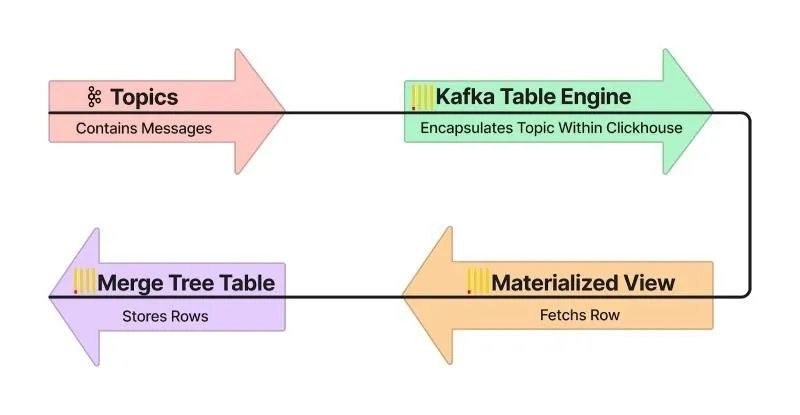
\includegraphics[width=1\textwidth]{../Images/SpecificaTecnica/enginePipeline.jpg}
  \caption{Data pipeline - ClickHouse}
  \label{fig:datapip}
\end{figure}

\paragraph{MergeTree}\label{sec:MergeTree}
Link alla documentazione: \href{https://clickhouse.com/docs/en/engines/table-engines/mergetree-family/mergetree#mergetree}{ClickHouse - MergeTree} (Consultato 25/03/2024).\newline
MergeTree è uno dei motori di archiviazione di base più utilizzati in ClickHouse. È progettato per gestire dati ordinati in append-only e offre un'ottima combinazione di prestazioni di lettura, scrittura, scalabilità e funzionalità per diversi casi d'uso.
Caratteristiche principali:
\begin{itemize}
  \item \textbf{Ordinato}: I dati sono archiviati in ordine crescente in base alla chiave di ordinamento specificata;
  \item \textbf{Append-only}: I nuovi dati vengono sempre aggiunti alla fine della tabella;
  \item \textbf{Scalabile}: Altamente scalabile orizzontalmente;
  \item \textbf{Partizionamento}: Supporto per partizionare la tabella in base a una colonna specifica;
  \item \textbf{TTL (Time to Live)}: Consente di definire un TTL per i dati, eliminandoli automaticamente dopo un periodo di tempo specificato;
  \item \textbf{Compressione}: Supporta diverse tecniche di compressione per ridurre lo spazio di archiviazione utilizzato.
\end{itemize}

Casi d'uso comuni:
\begin{itemize}
  \item \textbf{Analisi di log};
  \item \textbf{Dati sensoriali};
  \item \textbf{Dati finanziari};
  \item \textbf{Dati di monitoraggio};
  \item \textbf{Time series data}.
\end{itemize}

Vantaggi:
\begin{itemize}
  \item \textbf{Prestazioni di lettura e scrittura elevate};
  \item \textbf{Scalabilità};
  \item \textbf{Funzionalità avanzate};
  \item \textbf{Adatto a diversi casi d'uso}.
\end{itemize}

\paragraph{Time To Live in ClickHouse} \label{sec:RollupTTL}
Link alla documentazione: \href{https://clickhouse.com/docs/en/guides/developer/ttl#implementing-a-rollup}{https://clickhouse.com/docs/en/guides/developer/ttl\#implementing-a-rollup} \newline

TTL (time-to-live) si riferisce alla capacità di spostare, eliminare o eseguire il rollup di righe o colonne dopo che è trascorso un determinato intervallo di tempo. Sebbene l'espressione "time-to-live" sembri applicarsi solo all'eliminazione di vecchi dati, TTL ha diversi casi d'uso:
\begin{itemize}
  \item \textbf{Eliminazione dei vecchi dati}: rimuovere i dati dopo un certo periodo di tempo;
  \item \textbf{Spostamento dei dati tra dischi}: spostare i dati tra volumi di archiviazione dopo un certo periodo di tempo;
  \item \textbf{Rollup dei dati}: raggruppare i dati più vecchi in varie aggregazioni e calcoli utili .
\end{itemize}

Nel progetto è stato fatto utilizzo dove opportuno dell'operazione di Rollup di misurazioni dei sensori.
Nello specifico dopo un certo intervallo di tempo non vengono piu conservate tutte le misurazioni di un sensore, ma solo una misurazione aggregata per ogni sensore e per ogni periodo di tempo specificato. Questo permette di ridurre il volume di dati da analizzare e di mantenere comunque un'informazione utile per l'analisi.

\paragraph{Partition}\label{sec:Partition}
Link alla documentazione: \href{https://clickhouse.com/docs/en/engines/table-engines/mergetree-family/mergetree#partition-by}{ClickHouse - Partitioning} (Consultato 25/03/2024).\\
Le partizioni sono una funzionalità fondamentale di ClickHouse che consente di organizzare in modo efficiente e gestire grandi volumi di dati. Questa funzionalità permette di suddividere i dati in gruppi logici in base a criteri specifici, come il valore di una colonna o un intervallo di tempo. Grazie a questa organizzazione ottimizzata, le query che richiedono l'accesso a dati specifici all'interno di una partizione possono essere eseguite rapidamente, garantendo prestazioni elevate anche su dataset di grandi dimensioni.\\

Le partizioni rappresentano uno strumento particolarmente utile quando si lavora con dati di serie temporali. La decisione sull'utilizzo del partizionamento dovrebbe derivare da una serie di considerazioni chiave:
\begin{itemize}
  \item \textbf{Interrogazione singola:} È previsto che le query siano principalmente focalizzate su una singola partizione? Ad esempio, se le interrogazioni tendono a riguardare risultati entro un periodo specifico come un giorno o un mese, sarebbe vantaggioso partizionare i dati in base a tali periodi temporali.
  \item \textbf{Scadenza dei dati (TTL):} Si desidera applicare una politica di Time-To-Live (TTL) ai dati, in modo che una volta che una partizione raggiunge una certa età, venga applicata un'azione specifica su di essa?
\end{itemize}

Spesso si consiglia di mantenere il numero di partizioni al di sotto di circa 100. Anche se è tecnicamente possibile utilizzare fino a 1000 partizioni, tale approccio potrebbe non essere ottimale e potrebbe influenzare le prestazioni del sistema, inclusi tempi di avvio, tempi di inserimento/query e l'utilizzo di memoria. Questo è dovuto all'impatto che un elevato numero di partizioni può avere sul file system e sulle dimensioni dell'indice, con conseguente aumento della complessità gestionale e dei carichi di lavoro.

Nel progetto viene fatto utilizzo del partizionamento temporale nelle tabelle in cui è ritenuto oppurtuno in base alle considerazioni sopra descritte.
Infatti l'utilizzo delle partizioni nel nostro contesto viene giustificato anche dall'utilizzo di un TTL (Time To Live),oltre che dal fatto che le interrogazzioni riguardino principalmente una singola partizione. infatti l'utilizzo combinato di queste due funzionalità consente:
\begin{itemize}
    \item Una gestione efficace dei dati nel tempo;
    \item Migliori prestazioni del sistema;
\end{itemize}

Il partizionamento basato sul timestamp,come detto, è una pratica comune in ClickHouse, poiché consente di organizzare i dati in partizioni in base al periodo temporale, ad esempio mensilmente. Questo approccio ottimizza l'archiviazione e facilita l'analisi dei dati di serie temporali, come le temperature o i log di eventi. Grazie a questa struttura, le query che coinvolgono dati all'interno di specifici intervalli temporali diventano più efficienti, consentendo un accesso rapido e una migliore analisi dei dati.
    
\paragraph{Projection}\label{sec:projections}
Link alla documentazione: \href{https://clickhouse.com/docs/en/sql-reference/statements/alter/projection}{https://clickhouse.com/docs/en/sql-reference/statements/alter/projection}\newline
Altra fonte utile: \href{https://presentations.clickhouse.com/percona2021/projections.pdf}{https://presentations.clickhouse.com/percona2021/projections.pdf} (Consultato 25/03/2024). \newline

Le projection in ClickHouse sono una funzionalità di ottimizzazione per migliorare le prestazioni delle query su tabelle MergeTree. Esse creano delle viste pre-aggregate o pre-ordinate dei dati originali, consentendo a ClickHouse di accedere e analizzare i dati in modo più efficiente.
Questa funzionalità è utile per:

\begin{itemize}
    \item Eseguire \textit{Query} basate su di una colonna che non fa parte della chiave primaria;
    \item Pre-aggregare colonne, riducendo sia i calcoli che l'I/O.
\end{itemize}

Come funzionano le projection:
\begin{itemize}
  \item \textbf{Definizione}: Si definisce una projection su una tabella MergeTree esistente. La projection specifica una sottocategoria di colonne e, opzionalmente, un nuovo ordine di ordinamento per queste colonne;
  \item \textbf{Creazione interna}: ClickHouse crea internamente una nuova tabella nascosta che contiene i dati della projection;
  \item \textbf{Aggregazione o ordinamento}: I dati selezionati vengono aggregati (utilizzando funzioni come media, somma, ecc.) o ordinati in base alle colonne specificate nella definizione della projection;
  \item \textbf{Selezione automatica}: Durante l'esecuzione di una query, ClickHouse analizza la projection e la tabella originale. Se la projection rientra nei criteri di selezione della query (colonne e ordine), ClickHouse può utilizzare la projection per rispondere alla query, evitando di accedere alla tabella originale completa.
\end{itemize}

Vantaggi delle projection:
\begin{itemize}
  \item \textbf{Miglioramento delle prestazioni}: Accedendo ai dati pre-aggregati o pre-ordinati, le query possono essere eseguite più velocemente;
  \item \textbf{Riduzione dell'utilizzo della CPU}: Le aggregazioni e gli ordinamenti vengono eseguiti durante la creazione della projection, riducendo il carico di lavoro della CPU durante le query;
  \item \textbf{Più flessibilità di query}: Le projection possono supportare ordini diversi rispetto alla tabella originale, aumentando la flessibilità delle query.
\end{itemize}
Casi d'uso comuni delle projection:
\begin{itemize}
  \item \textbf{Analisi di dati aggregati}: Se le query spesso richiedono aggregazioni come medie, somme o conteggi su specifici sottoinsiemi di colonne, le projection pre-aggregate possono migliorare le prestazioni;
  \item \textbf{Query con ordini specifici}: Se le query spesso filtrano e ordinano i dati in base a colonne specifiche, le projection pre-ordinate possono essere vantaggiose.
\end{itemize}

Svantaggi delle projection:
\begin{itemize}
  \item \textbf{Complessità di gestione}: È necessario definire e gestire le projection, aggiungendo complessità all'amministrazione del database;
  \item \textbf{Sovraccarico di scrittura}: La creazione e l'aggiornamento delle projection richiedono risorse di scrittura aggiuntive;
  \item \textbf{Spazio di archiviazione aggiuntivo}: Le projection occupano spazio di archiviazione aggiuntivo rispetto alla tabella originale.
\end{itemize}

Nel contesto del progetto, le proiezioni sono state impiegate strategicamente al fine di ottimizzare le prestazioni delle interrogazioni basate sulla colonna "\textit{cella}". Questa colonna, pur non facendo parte della chiave primaria, è oggetto di interrogazioni molto frequenti su vasti volumi di dati.

L'adozione di proiezioni consente di migliorare l'efficienza delle interrogazioni, consentendo al sistema di recuperare rapidamente e gestire in modo ottimale i dati relativi alla colonna "\textit{cella}". Tale strategia si rivela particolarmente vantaggiosa vista la previsione di interrogazioni ricorrenti e su dataset di grandi dimensioni basate su tale colonna, contribuendo così a garantire tempi di risposta ottimizzati e una migliore esperienza utente.


In generale l'introduzione delle PROJECTIONS produce risultati di notevole importanza, come illustrato di seguito. Consideriamo una tipica query eseguita per l'analisi tramite Grafana:
    
    \begin{lstlisting}[caption={Query tipica - Grafana}, captionpos=b]
      SELECT ID_sensore, avgMerge(value) AS value, timestamp
      FROM innovacity.temperatures
      WHERE (cella IN ('Arcella')) AND ((timestamp >= toDateTime64(1708338633507 / 1000, 3)) AND (timestamp <= toDateTime64(1708338933507 / 1000, 3) + INTERVAL 1 DAY))
      GROUP BY timestamp, ID_sensore
      HAVING (value >= -100) AND (value <= 100)

      --Query id: 48635435-9b35-4727-b580-9e33a9db92d4
    \end{lstlisting}

    \begin{figure}[H]
        \centering
        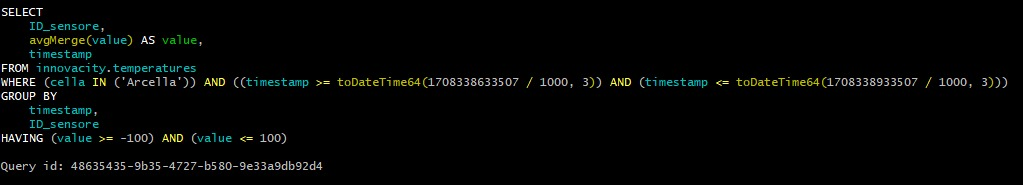
\includegraphics[width=1\textwidth]{../Images/SpecificaTecnica/ProjectionQuery.jpg}
        \caption{Query tipica - Grafana}
        \label{fig:ProjectionsQuery}
      \end{figure}
      Senza l'utilizzo delle PROJECTIONS, il risultato ottenuto è il seguente:
    \begin{figure}[H]
        \centering
        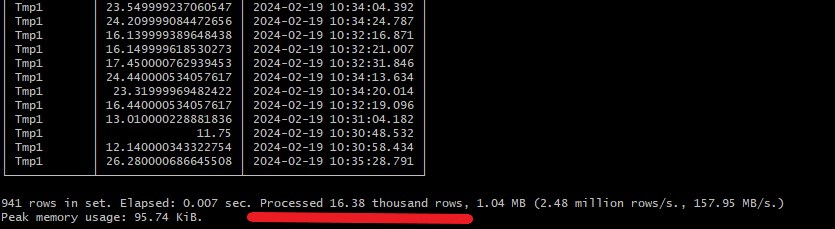
\includegraphics[width=0.9\textwidth]{../Images/SpecificaTecnica/SenzaProectionResult.jpg}
        \caption{Query tipica risultato senza projections}
        \label{fig:ProjectionsQueryWthout}
      \end{figure}
      ovvero sono state processate per ottenere il risultato della query \textbf{16,38} migliaia di righe. Invece in seguito all’aggiunta delle PROJECTIONS:

      \begin{figure}[H]
        \centering
        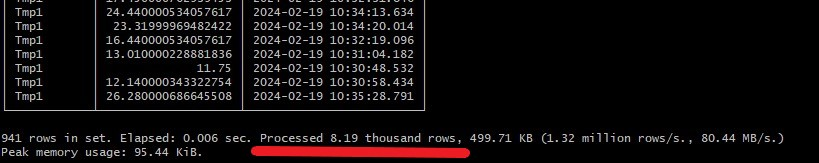
\includegraphics[width=0.9\textwidth]{../Images/SpecificaTecnica/ConProjectionRisultato.jpg}
        \caption{Query tipica risultato con projections}
        \label{fig:ProjectionsQueryWith}
      \end{figure}   
  Sono state elaborate approssimativamente \textbf{8,19} migliaia di righe per ottenere il risultato della query, circa la metà rispetto al conteggio precedente, evidenziando un miglioramento significativo. Inoltre, mediante un'interrogazione specifica è possibile confermare che le PROJECTIONS sono state effettivamente impiegate per generare il risultato della query in questione.
\begin{figure}[H]
    \centering
    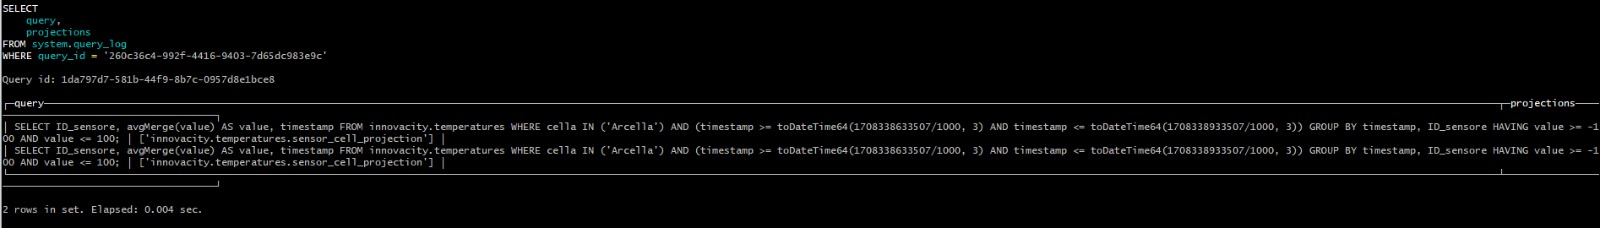
\includegraphics[width=1\textwidth]{../Images/SpecificaTecnica/ProjectionUsedByClickHouse.jpg}
    \caption{Uso della Projection}
    \label{fig:ProjectionsUsed}
\end{figure}

Considerando un'altra query eseguita dall'applicativo, che calcola la media globale di \textbf{170.000} misurazioni di temperatura, è possibile riconoscere i benefici derivanti dall'utilizzo delle PROJECTIONS. Alla conclusione dell'analisi, è evidente anche il loro effettivo impiego nel calcolo del risultato. Grazie all'adozione delle PROJECTIONS, si ottiene:
\begin{figure}[H]
    \centering
    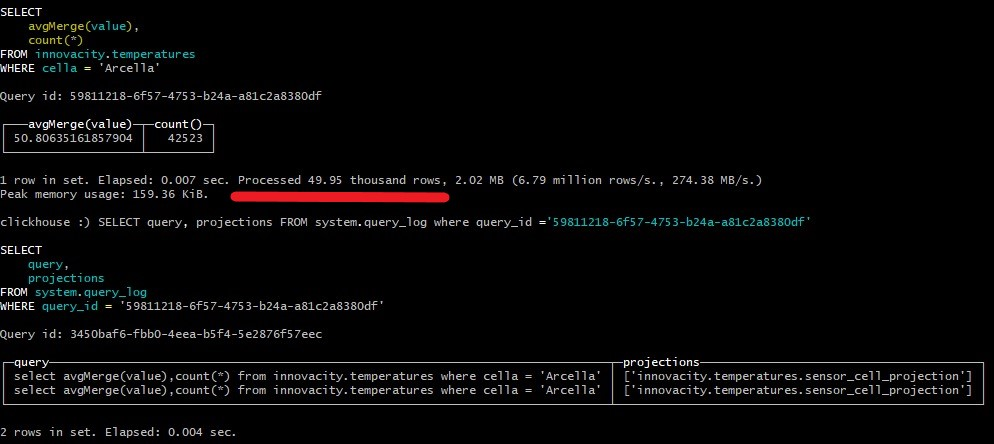
\includegraphics[width=1\textwidth]{../Images/SpecificaTecnica/query2ProjectionsWith.jpg}
    \caption{Query esempio Projection 2 - ClickHouse}
    \label{fig:with2proj}
  \end{figure}
Ovvero il totale di righe processate per ottenere il risultato è di \textbf{49,95 migliaia} con \textbf{0,07 secondi} di tempo utilizzati.
Si puo notare invece la differenza delle righe processate una volta rimossa la \textit{PROJECTIONS}:
\begin{figure}[H]
    \centering
    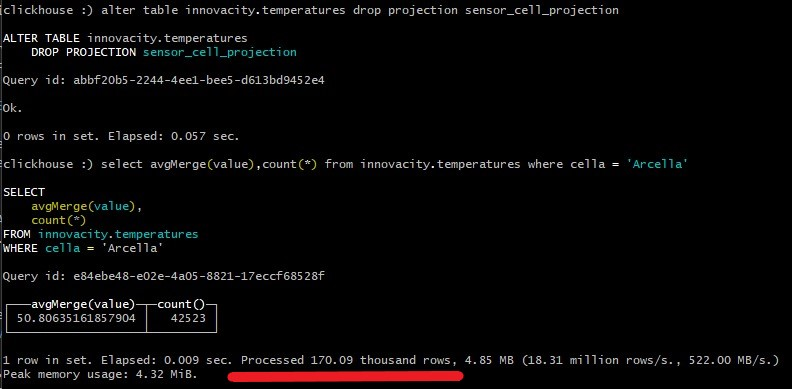
\includegraphics[width=1\textwidth]{../Images/SpecificaTecnica/query2ProjectionsWithout.jpg}
    \caption{Query esempio senza Projection 2 - ClickHouse}
    \label{fig:without2proj}
  \end{figure}

 Il totale di righe processate per ottenere il risultato è ora di \textbf{170,09 migliaia}, ovvero la totalità delle righe presenti nella tabella, con \textbf{0,09 secondi} di tempo utilizzati.

\subsubsection{Integrazione Kafka tramite Kafka Engine in ClickHouse}\label{sec:kafka_engine}
ClickHouse supporta l'integrazione con Kafka tramite Kafka Engine, permettendo la lettura dei dati da un topic Kafka e il loro salvataggio in una tabella ClickHouse adatta a grandi dataset. Tale funzionalità riveste un'importanza notevole per applicazioni che richiedono l'elaborazione in tempo reale di dati provenienti da fonti esterne, una necessità frequente nel contesto del monitoraggio urbano. L'integrazione con Kafka consente l'acquisizione e la memorizzazione efficiente dei dati, garantendo prestazioni elevate anche su grandi volumi di dati.\\
Kafka Engine è progettato per il recupero di dati una sola volta. Ciò significa che una volta che i dati vengono interrogati da una tabella Kafka, vengono considerati consumati dalla coda. Pertanto, non si dovrebbero mai selezionare dati direttamente da una tabella di Kafka Engine, ma utilizzare invece una vista materializzata. Una vista materializzata viene attivata una volta che i dati sono disponibili in una tabella di Kafka Engine. Automaticamente sposta i dati da una tabella Kafka a una tabella di tipo MergeTree o Distributed. Quindi, sono necessarie almeno 3 tabelle:
\begin{itemize}
  \item La tabella di origine del motore Kafka;
  \item La tabella di destinazione (famiglia MergeTree o distribuita);
  \item Vista materializzata per spostare i dati;
\end{itemize}
\begin{figure}[H]
  \centering
  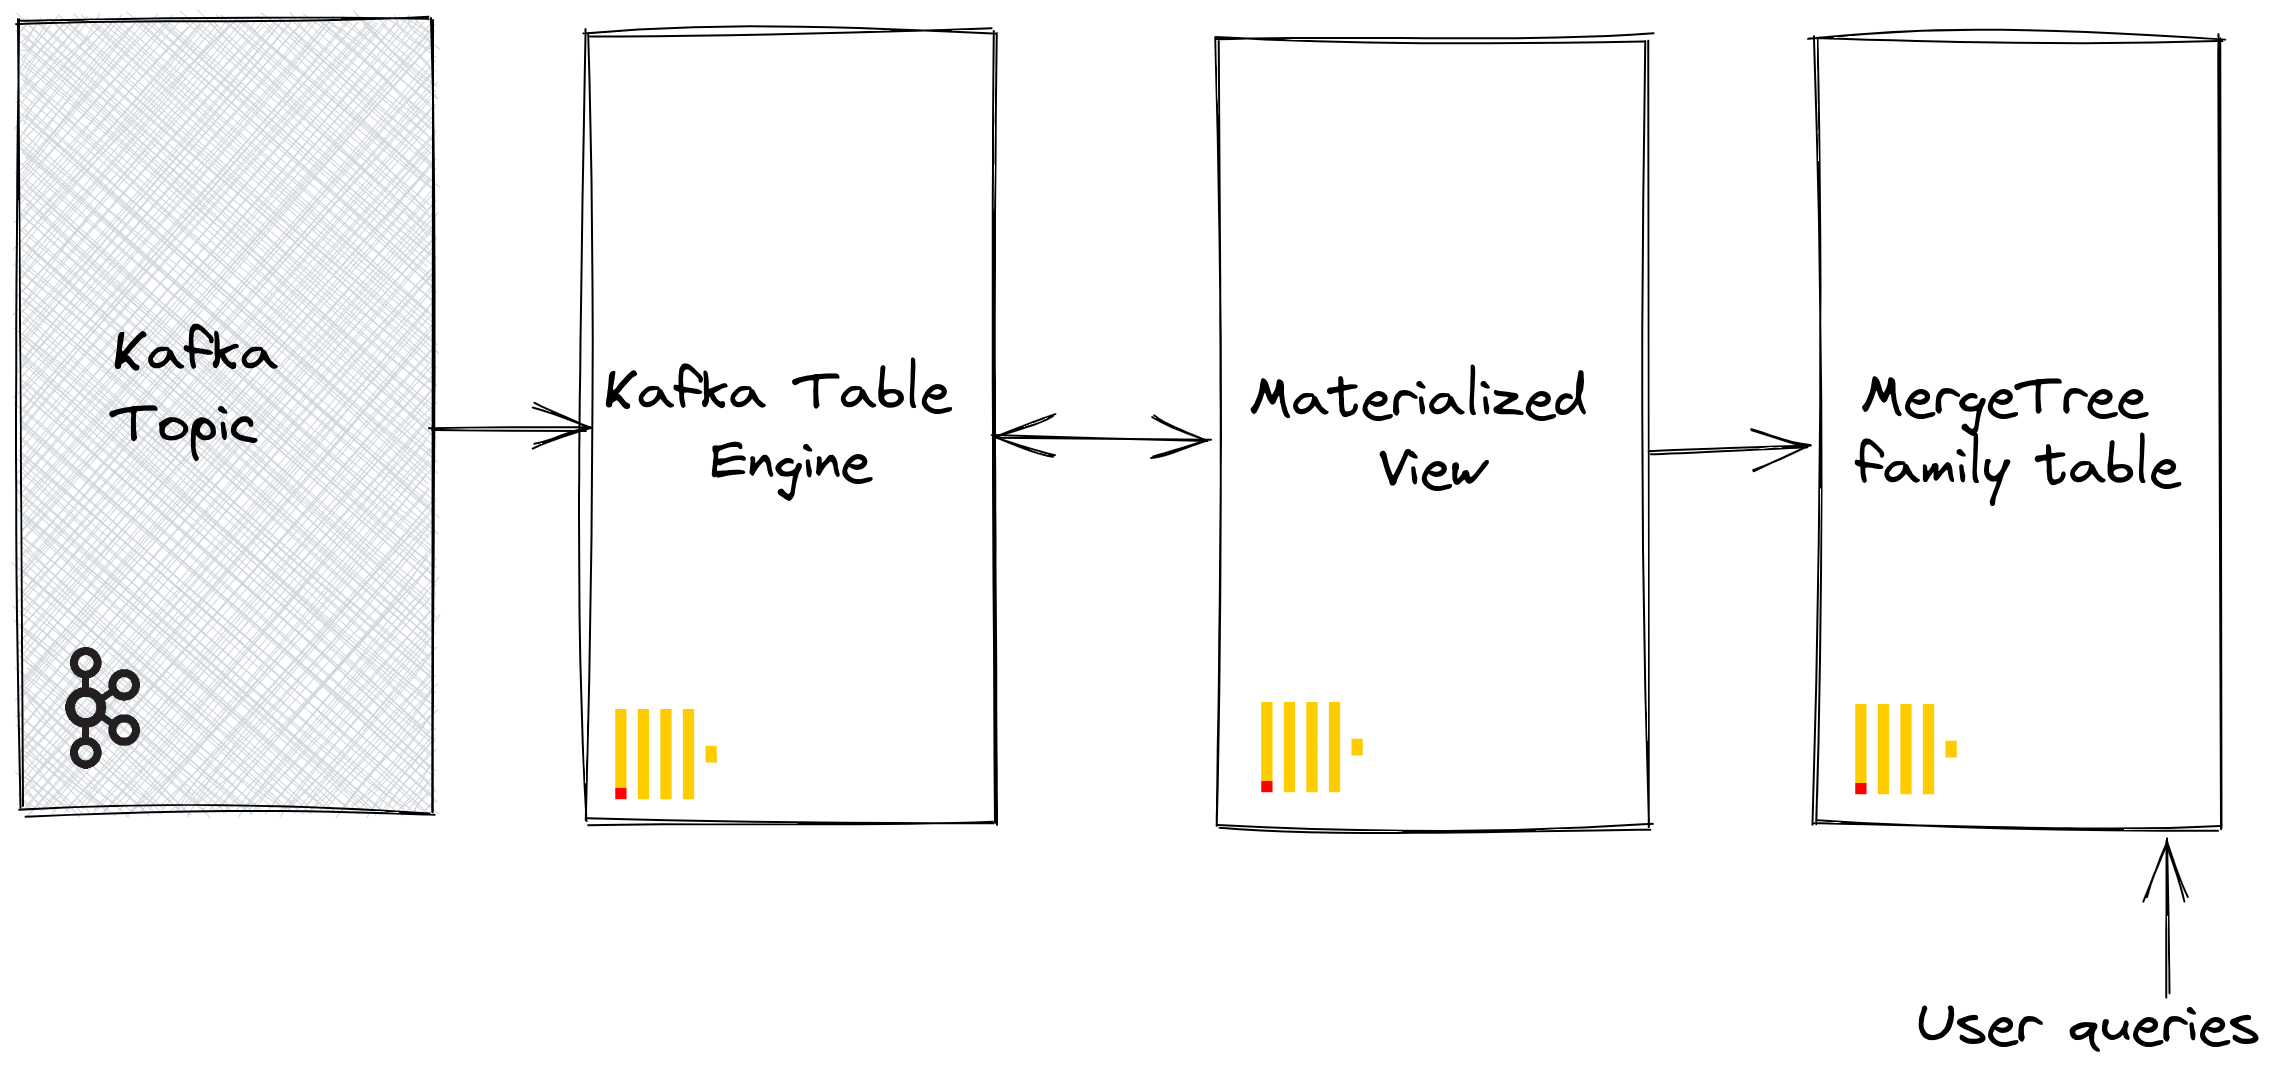
\includegraphics[width=.7\textwidth]{../Images/SpecificaTecnica/kafka_engine_architecture.png}
  \caption{Architettura di Kafka Engine in ClickHouse}
  \label{fig:Architettura_kafka_engine}
\end{figure}

\subsubsection{Trasferimento dati tramite Materialized View} \label{sec:materializedView}
Una materialized view funge da ponte tra la fonte dei dati (Kafka Engine) e la destinazione dei dati (MergeTree). Quando nuovi dati vengono scritti nella tabella Kafka Engine, la materialized view viene attivata automaticamente.\\
La materialized view esegue una query sulla tabella Kafka Engine per selezionare i dati più recenti. Una volta selezionati, questi dati vengono inseriti nella tabella di destinazione (ad esempio, una tabella MergeTree). Questo processo avviene in modo automatico e immediato, senza bisogno di intervento manuale.\\
In pratica, la materialized view si assicura che la tabella di destinazione sia sempre aggiornata con i dati più recenti presenti nella tabella Kafka Engine. Questo offre numerosi vantaggi:
\begin{itemize}
  \item \textbf{Automatizzazione del processo}: Non è necessario eseguire manualmente operazioni di trasferimento dati da una tabella all'altra. La materialized view si occupa di tutto in modo automatico;
  \item \textbf{Efficienza}: Il trasferimento dei dati avviene in tempo reale, garantendo che la tabella di destinazione sia sempre allineata con la fonte dei dati senza ritardi;
  \item \textbf{Ottimizzazione delle risorse}: Il processo di trasferimento dei dati è gestito in modo efficiente, utilizzando al meglio le risorse disponibili e garantendo prestazioni elevate.
\end{itemize}
Nel contesto specifico, le materialized view sono responsabili di eseguire controlli sui dati, come ad esempio la verifica della loro correttezza ed affidabilità nel contesto di utilizzo, prima di inserirli nella tabella di destinazione. Questo processo assicura che i dati siano sempre affidabili e pronti per l'analisi, senza la necessità di ulteriori operazioni di pulizia o preparazione.\\
Per esempio, nel caso dei dati di umidità raccolti da sensori in un'area urbana, la materialized view potrebbe eseguire controlli per assicurarsi che i valori rientrino all'interno di un intervallo plausibile e che non ci siano discrepanze improbabili. Ciò garantirebbe che i dati di umidità inseriti nella tabella di destinazione siano accurati e affidabili per l'analisi meteorologica o ambientale.


\subsubsection{Tabella Kafka Engine per un sensore generico}
Le tabelle del database impiegate per ottenere le misurazioni di ciascuna tipologia di sensore dai topic kafka presentano una configurazione sostanzialmente simile, differenziandosi principalmente per il tipo di dato della colonna relativa alla misurazione e per il \textit{topic} di riferimento utilizzato per ottenere le misurazioni.
Nello specifico per ogni sensore si avrà la seguente tabella Clickhouse:
\begin{figure}[H]
    \centering
    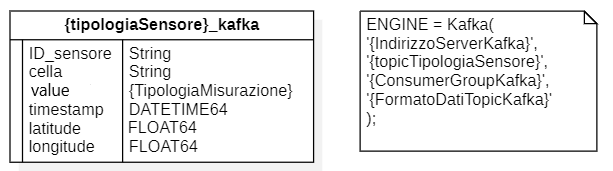
\includegraphics[width=.6\textwidth]{../Images/SpecificaTecnica/sensorType_kafka.PNG}
    \caption{Tabella sensore generico per il reperimento da kafka - ClickHouse}
    \label{fig:Reperimento_kafka_clickhouse}
  \end{figure}

    La tabella è configurata con il motore di storage Kafka, il che significa che i dati verranno letti da un \textit{topic Kafka}. 

    I campi sono:
    \begin{itemize}
        \item \textbf{ID\_sensore}: un campo di tipo \textit{String} che identifica univocamente il sensore che ha effettuato la misurazione;
        \item \textbf{cella}: un campo di tipo \textit{String} che rappresenta la cella della città in cui è stata effettuata la misurazione;
        \item \textbf{value}: un campo di tipo variabile a seconda del tipo di misurazione che contiene il valore della temperatura;
        \item \textbf{timestamp}: campo di tipo \textit{DATETIME64} che rappresenta il timestamp della misurazione della temperatura;
        \item \textbf{latitude}: un campo di tipo \textit{Float64} che rappresenta la latitudine del luogo dove è stata effettuata la misurazione;
        \item \textbf{longitude}: un campo di tipo \textit{Float64} che rappresenta la longitudine del luogo dove è stata effettuata la misurazione.
    \end{itemize}

    Mentre i parametri esposti racchiusi da parentesi graffe variano per ogni tipolgia di sensore correlato alla misurazione e sono:
    \begin{itemize}
        \item \textbf{tipologiaSensore}: viene sostituito con la tipologia del sensore che effettua le misurazioni salvate nella tabella; (ex. temperatures)
        \item \textbf{TipoDatoMisurazione}: viene sostituito con il tipo del dato che rappresenta la misurazione (ex. Float32, UInt8);
        \item \textbf{IndirizzoServerKafka}: specifica l'indirizzo del server Kafka.
        Nel nostro caso il server Kafka è in esecuzione su un container \textit{Docker} raggiungibile tramite l'indirizzo:
         \textit{'kafka:9092'};
        \item \textbf{topicTipologiaSensore}: specifica il nome del topic Kafka da cui leggere i dati (ex.temperature). Accetta anche liste di topic Kafka separati da virgole.
        \item \textbf{ConsumerGroupKafka}: specifica il nome del consumer group Kafka che verrà utilizzato per leggere i messaggi dal topic Kafka denominato 'temperature'.
        Un consumer group in Kafka è un gruppo di consumatori che lavorano insieme per consumare i messaggi da uno o più topic. Ogni messaggio inviato a un \textit{topic Kafka} può essere consumato da uno dei consumatori nel gruppo. I consumer all'interno di uno stesso gruppo condividono l'elaborazione dei messaggi all'interno dei topic: ogni messaggio viene elaborato da uno e un solo consumatore all'interno del gruppo. Nel nostro caso sarà sempre '\textit{CG\_Clickhouse\_1}' per indicare il servizio di salvataggio \textit{Clickhouse}.
        \item \textbf{FormatoDatiTopicKafka}: specifica il formato dei dati nel \textit{topic Kafka}. Nel nostro caso, i dati sono nel formato JSONEachRow, che è un formato di serializzazione JSON di \textit{ClickHouse} che consente di scrivere o leggere record JSON separati da una riga. Quindi avremo che <<FormatoDatiTopicKafka>> = \textit{JSONEachRow}.
        \item \textbf{KafkaSkipBrokenMessages}:
        \begin{itemize}
          \item è un'opzione di configurazione utilizzata nel motore Kafka di ClickHouse. Determina il comportamento del motore quando incontra messaggi Kafka considerati "corrotti" o non processabili.
          Un messaggio Kafka può essere considerato corrotto per diversi motivi, tra cui:
          \begin{itemize}
            \item \textbf{Formato non valido}: Il messaggio potrebbe avere un formato JSON o Avro non valido, impedendo a ClickHouse di decodificarlo correttamente.
            \item \textbf{Dati mancanti}: Il messaggio potrebbe contenere dati mancanti o incompleti, violando lo schema previsto.
            \item \textbf{Errori di codifica}: Il messaggio potrebbe avere errori di codifica che impediscono la lettura dei dati.
          \end{itemize}
         \item Per impostazione predefinita, \textit{kafka\_skip\_broken\_messages} è impostato su 0. Ciò significa che ClickHouse interrompe l'elaborazione del flusso di dati da Kafka e registra un errore quando incontra un messaggio corrotto.
        \item Puoi configurare \textit{kafka\_skip\_broken\_messages} su un valore diverso da zero per modificare il comportamento. Il valore rappresenta il numero massimo di messaggi corrotti consecutivi per blocco, considerato nel contesto di  \textit{kafka\_max\_block\_size}, che ClickHouse ignorerà prima di interrompere l'elaborazione.
        \item Bisogna anche ricordare che per come è stato progettato il sistema i messaggi corrotti vengono scartati "alla fonte" dallo Schema Registry di Kafka.
        \item Nel nostro caso vogliamo che ogni messaggio malformato nel blocco venga ignorato.
        \end{itemize}
        \item \textbf{input\_format\_skip\_unknown\_fields}:  è un'impostazione utilizzata con alcuni formati di input di ClickHouse, compreso quello da noi utilizzato \textit{JSONEachRow} per specificare come gestire i dati in entrata che contengono colonne sconosciute alla tabella di destinazione. Impostando \textit{input\_format\_skip\_unknown\_fields} su 1, ClickHouse ignorerà le colonne sconosciute nei dati in entrata e importerà solo le colonne che corrispondono alle colonne della tabella di destinazione. Questo è utile quando si desidera importare solo una parte dei dati in entrata, ignorando le colonne non necessarie o non rilevanti.
        Nel nostro caso l'impostazione di default è quella richiesta.
    \end{itemize}

   %_____________________________________________________________________________
 
    \subsubsection{Misurazioni temperatura} \label{sec:tab_temperatures}
    Di seguito viene presentata una configurazione dettagliata per l'archiviazione delle misurazioni di temperatura. Tale configurazione, progettata per acquisire dati da un topic Kafka permette la persistenza delle misurazioni di temperatura che include l'ID del sensore (String), la cella della città da cui proviene la misurazione(String), la temperatura misurata (Float32), il timestamp della misurazione (DATETIME64), la latitudine (Float64) e la longitudine (Float64) del sensore. La tabella di destinazione è denominata 'temperatures' e utilizza il motore di storage MergeTree, che è ottimizzato per l'archiviazione e l'analisi di dati cronologicamente ordinati in append-only (I nuovi dati vengono sempre aggiunti alla fine della tabella e i dati esistenti non vengono modificati). Questa scelta è giustificata dal fatto che le misurazioni di temperatura sono tipicamente ordinate cronologicamente e richiedono l'accesso a dati specifici all'interno di un intervallo di tempo definito.
    Da osservare che l'attributo presente nel messaggio JSON : "\textit{type}" viene ignorato, poichè non necessario in una tabella dedicata alle sole misurazioni di temperatura. Ciò accade grazie al valore di deault dell'impostazione \textit{input\_format\_skip\_unknown\_fields} della tabella con motore kakfa.
    Vengono definite come \textit{PRIMARY KEY} le colonne \textit{ID\_sensore} e \textit{timestamp} per garantire l'unicità delle misurazioni e la possibilità di effettuare ricerche efficienti.

    \begin{figure}[H]
        \centering
        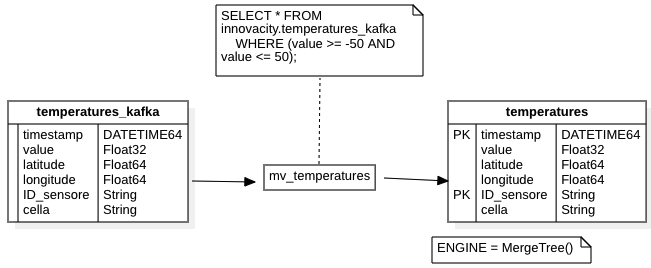
\includegraphics[width=1\textwidth]{../Images/SpecificaTecnica/temperatures.png}
        \caption{Tabella temperatures\_kafka e temperatures}
        \label{fig:temperatures}
      \end{figure}
    
    La tabella 'temperatures\_kafka' come spiegato in precedenza funge da tramite tra il topic Kafka relativo alle misurazioni di temperatura e il sistema di gestione dei dati ClickHouse. Questa tabella agisce come un'interfaccia trasformando i flussi di dati provenienti dal topic Kafka in un formato comprensibile per ClickHouse. Successivamente, una Materialized View, in questo caso 'mv\_temperatures', opera su questa tabella per trasferire i dati ottenuti verso la tabella di destinazione 'temperatures' della famiglia MergeTree come spiegato in \ref{sec:materializedView}.
    
\paragraph{Projections per misurazioni di temperatura} \label{sec:temp_projections}
Durante la fase di progettazione, è stata dedicata particolare attenzione all'utilizzo delle tabelle precedentemente descritte e alle richieste che verranno formulate su di esse. È emerso che, considerando il requisito di suddividere la città in una serie di celle e specificare la cella di origine della misurazione, la filtrazione delle misurazioni per celle diventerà una richiesta frequente al database. Di conseguenza, si è optato per l'utilizzo delle PROJECTIONS per ottimizzare il filtering su tale campo, le quali sono dettagliatamente descritte nella sezione \ref{sec:projections}.
\vspace{0,3cm}
\begin{lstlisting}[caption={implementazione PROJECTION tabella temperatures}, captionpos=b]
  --Projection per tabella temperatures
  ALTER TABLE innovacity.temperatures ADD PROJECTION tmp_sensor_cell_projection (SELECT * ORDER BY cella);
  ALTER TABLE innovacity.temperatures MATERIALIZE PROJECTION tmp_sensor_cell_projection;
\end{lstlisting}
\vspace{0,3cm}
La proiezione ci consentirà di effettuare rapidamente filtraggi basati sulle celle, anche se tale attributo non è definito come \textit{PRIMARY\_KEY} nella tabella originale.
      
  \paragraph{TTL per misurazioni di temperatura} \label{sec:temp_projections}
  L'implementazione del Time to Live (TTL) di Rollup per le misurazioni di temperatura deve permettere di salvare un solo dato aggregato per ora e per sensore dopo che è trascorso più di un mese dal timestamp della misurazione.
  \begin{lstlisting}[caption={implementazione TTL tabella temperatures}, captionpos=b]
    TTL toDateTime(timestamp) + INTERVAL 1 MONTH
      GROUP BY ID_sensore,toStartOfHour(timestamp)
      SET
          value = avg(value);
  \end{lstlisting}

\paragraph*{Partition per misurazioni di temperatura}\label{sec:temp_part}
La tabella è partizionata per anno e mese in base al valore della colonna timestamp. Ciò significa che i dati vengono archiviati in parti separate per ogni combinazione di anno e mese. Questo approccio consente di organizzare i dati in modo efficiente e di eseguire query su intervalli temporali specifici in modo rapido ed efficiente. Inoltre, il partizionamento per anno e mese consente di applicare il TTL in modo selettivo.
La scelta sull'utilizzo delle Partition e sulla relativa configurazione è stata dettata dalle considerazioni esposte in \ref{sec:Partition}.

%_____________________________________________________________________________

\subsubsection{Misurazioni umidità}
Le considerazioni relative al salvataggio delle misurazioni di umidità coincidono con quelle espresse nella sezione \ref{sec:temp_projections} riguardo alle misurazioni di temperatura.
In questa situazione, dove le misure riguardano l’umidità, la tabella di destinazione ClickHouse è nominata ‘humidity’:
Il tipo della colonna \textit{value} è \textit{Float32} poichè il valore dell'umidità è in percentuale, compreso tra 0 e 100. Le altre colonne sono identiche a quelle della tabella 'temperatures' e sono definite con lo stesso tipo di dato per garantire la precisione e l'integrità dei dati.
\begin{figure}[H]
    \centering
    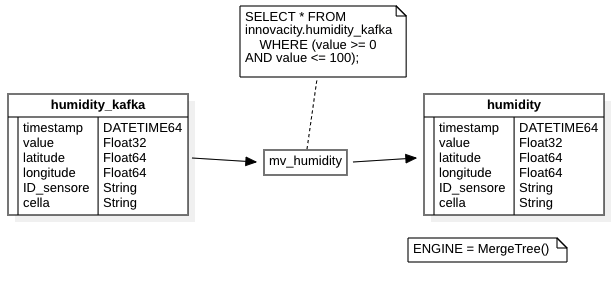
\includegraphics[width=1\textwidth]{../Images/SpecificaTecnica/humidity.png}
    \caption{Tabella humidity\_kafka e humidity}
    \label{fig:humidity_tables}
  \end{figure}

\paragraph{Projections per misurazioni di umidità} 
Dopo aver considerato le stesse argomentazioni presentate nella sezione \ref{sec:tab_temperatures} riguardanti le misurazioni di temperatura, abbiamo deciso di estendere l'utilizzo delle PROJECTION anche alle misurazioni di umidità. I vantaggi ottenuti risultano essere simili a quelli evidenziati per le misurazioni di temperatura, come descritto nella stessa sezione. A seguire, vengono illustrate le configurazioni delle PROJECTION relative alle tabelle delle misurazioni di umidità:

\begin{lstlisting}
    --Projection per tabella humidity
    ALTER TABLE innovacity.humidity ADD PROJECTION umd_sensor_cell_projection (SELECT * ORDER BY cella);
    ALTER TABLE innovacity.humidity MATERIALIZE PROJECTION umd_sensor_cell_projection;
\end{lstlisting}

\paragraph{Partition \& TTL per misurazioni di umidità}
La configurazione riguardante il partizionamento e il TTL per le misurazioni di umidità corrisponde a quella descritta nella sezione \ref{sec:temp_projections} e \ref{sec:temp_part} in merito alle misurazioni di temperatura.
%_____________________________________________________________________________

\subsubsection{Misurazioni di polveri sottili}
Le considerazioni concernenti l'archiviazione delle misurazioni di polveri sottili corrispondono a quelle espresse nella sezione \ref{sec:tab_temperatures} in merito alle misurazioni di temperatura.
Il tipo della colonna \textit{value} è \textit{Float32} poichè il valore delle polveri sottili è espresso in microgrammi per metro cubo (µg/m³), un valore compreso tra 0 e 1000. La tabella di destinazione ClickHouse è nominata ‘dustPM10’:
Le altre colonne sono identiche a quelle della tabella 'temperatures' e sono definite con lo stesso tipo di dato per garantire la precisione e l'integrità dei dati.
\begin{figure}[H]
    \centering
    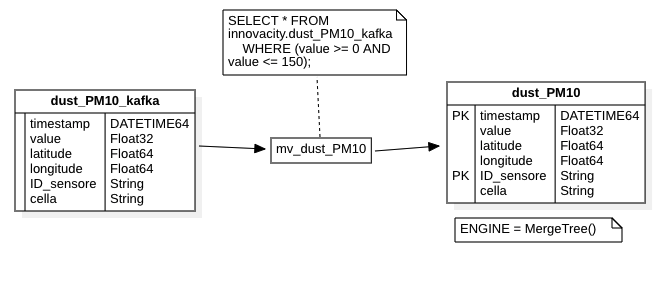
\includegraphics[width=1\textwidth]{../Images/SpecificaTecnica/dust_PM10.png}
    \caption{Tabella dustPM10\_kafka e dustPM10}
    \label{fig:dust_table}
  \end{figure}

\paragraph{Projections per misurazioni di polveri sottili} 
Dopo aver considerato le stesse argomentazioni presentate nella sezione \ref{sec:tab_temperatures} riguardanti le misurazioni di temperatura, abbiamo deciso di estendere l'utilizzo delle PROJECTION anche alle misurazioni di polveri sottili. I vantaggi ottenuti risultano essere simili a quelli evidenziati per le misurazioni di temperatura, come descritto nella stessa sezione. A seguire, vengono illustrate le configurazioni delle PROJECTION relative alle tabelle delle misurazioni di polveri sottili:

\begin{lstlisting}
  --Projection per tabella dust_PM10
  ALTER TABLE innovacity.dust_PM10 ADD PROJECTION dust_sensor_cell_projection (SELECT * ORDER BY cella);
  ALTER TABLE innovacity.dust_PM10 MATERIALIZE PROJECTION dust_sensor_cell_projection;
\end{lstlisting}

\paragraph{Partition \& TTL per misurazioni di polveri sottili}
La configurazione riguardante il partizionamento e il TTL per le misurazioni di umidità corrisponde a quella descritta nella sezione \ref{sec:temp_projections} e \ref{sec:temp_part} in merito alle misurazioni di temperatura.
%_____________________________________________________________________________
\subsubsection{Misurazioni isole ecologiche}
Le considerazioni concernenti l'archiviazione delle misurazioni delle isole ecologiche corrispondono a quelle espresse nella sezione \ref{sec:tab_temperatures} in merito alle misurazioni di temperatura. Il tipo della colonna \textit{value} è \textit{Float32} poichè il valore della misurazione riguarda la percentuale di riempimento, compreso tra 0 e 100. Le altre colonne sono identiche a quelle della tabella 'temperatures' e sono definite con lo stesso tipo di dato per garantire la precisione e l'integrità dei dati.

\begin{figure}[H]
  \centering
  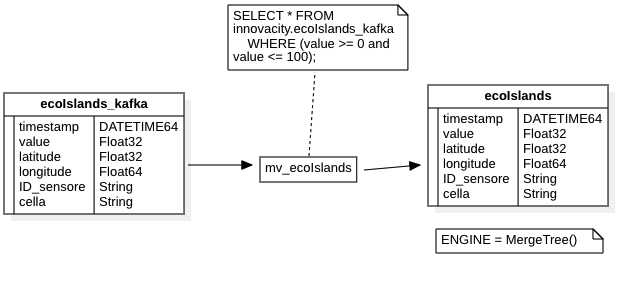
\includegraphics[width=1\textwidth]{../Images/SpecificaTecnica/ecoIslands.png}
  \caption{Tabella ecoIslands\_kafka e ecoIslands}
  \label{fig:ecoIslands_tables}
\end{figure}

\paragraph{Projections per misurazioni delle isole ecologiche} 
Dopo aver considerato le stesse argomentazioni presentate nella sezione \ref{sec:tab_temperatures} riguardanti le misurazioni di temperatura, abbiamo deciso di estendere l'utilizzo delle PROJECTION anche alle misurazioni delle isole ecologiche. I vantaggi ottenuti risultano essere simili a quelli evidenziati per le misurazioni di temperatura, come descritto nella stessa sezione. A seguire, vengono illustrate le configurazioni delle PROJECTION relative alle tabelle delle misurazioni delle isole ecologiche:

\begin{lstlisting}
  --Projection per tabella ecoIslands
  ALTER TABLE innovacity.ecoIslands ADD PROJECTION umd_sensor_cell_projection (SELECT * ORDER BY cella);
  ALTER TABLE innovacity.ecoIslands MATERIALIZE PROJECTION umd_sensor_cell_projection;
\end{lstlisting}

\paragraph{Partition \& TTL per misurazioni di umidità}
La configurazione riguardante il partizionamento e il TTL per le misurazioni di umidità corrisponde a quella descritta nella sezione \ref{sec:temp_projections} e \ref{sec:temp_part} in merito alle misurazioni di temperatura.

%_____________________________________________________________________________

\subsubsection{Misurazioni guasti elettrici} \label{sec:tab_guasti}
Le considerazioni concernenti l'archiviazione delle misurazioni dei guasti elettrici corrispondono a quelle espresse nella sezione \ref{sec:tab_temperatures} in merito alle misurazioni di temperatura.
Il tipo della colonna \textit{value} è \textit{UInt8} poichè il valore delle misurazioni dei guasti elettrici è binario, 0 (guasto rilevato) oppure 1 (guasto non rilevato). La tabella di destinazione ClickHouse è nominata ‘electricalFault’:
Le altre colonne sono identiche a quelle della tabella 'temperatures' e sono definite con lo stesso tipo di dato per garantire la precisione e l'integrità dei dati.

\begin{figure}[H]
    \centering
    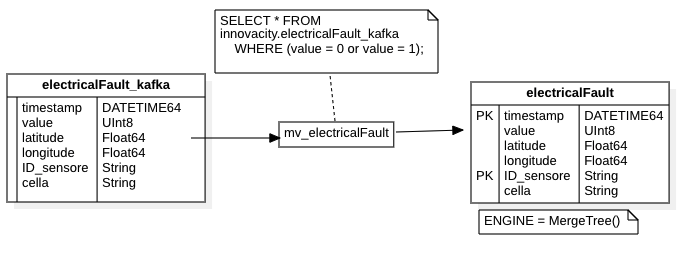
\includegraphics[width=1\textwidth]{../Images/SpecificaTecnica/electricalFault.png}
    \caption{Tabella electricalFault\_kafka e electricalFault}
    \label{fig:electricalFault_tables}
  \end{figure}


\paragraph{Considerazioni su Projection,Partition e TTL per misurazioni di guasti elettrici} 
Le proiezioni per questo tipo di misurazione non offrono la stessa utilità rispetto a quelle relative alla temperatura, dove spesso si eseguono analisi temporali su ampi periodi e grandi volumi di dati filtrati per cella.

In questo contesto di misurazione, le operazioni di selezione sulla tabella si concentrano sul recupero dell'ultimo valore registrato.

La creazione di una proiezione per questa tabella comporterebbe solo un sovraccarico di calcolo, IO e spazio su disco utilizzato, senza un reale vantaggio in termini di prestazioni o funzionalità.

Inoltre non si verificano le condizioni che giustifichino l'utilizzo del partizionamento (esposte in {sec:Partition}) e del Time-To-Live (TTL),  in quanto non avrebbe senso aggregare misurazioni di questo genere dopo un certo periodo di tempo che porterebbero a misurazioni prive di valore informativo o senza significato.
%_____________________________________________________________________________

\subsubsection{Misurazioni stazioni di ricarica} Le considerazioni concernenti l'archiviazione delle misurazioni delle stazioni di ricarica corrispondono a quelle espresse nella sezione \ref{sec:tab_guasti} in merito alle misurazioni guasti elettrici. Il tipo della colonna \textit{value} è \textit{UInt8} poichè il valore delle misurazioni delle stazioni di ricarica è binario, 0 (stazione di ricarica non occupata) oppure 1 (stazione di ricarica occupata). La tabella di destinazione ClickHouse è nominata ‘chargingStation’:

\begin{figure}[H]
    \centering
    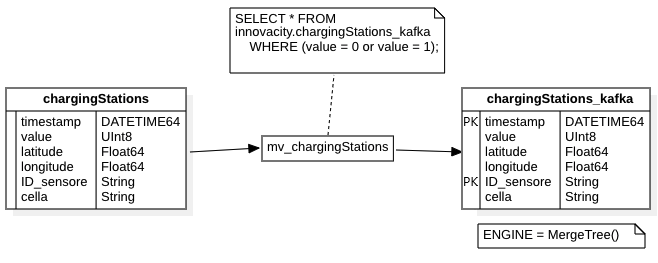
\includegraphics[width=1\textwidth]{../Images/SpecificaTecnica/chargingStations.png}
    \caption{Tabella chargingStation\_kafka e chargingStation}
    \label{fig:chargingStation_tables}
  \end{figure}
%_____________________________________________________________________________

\subsubsection{Misurazioni sensori di rilevameno dell’acqua}
Le considerazioni concernenti l'archiviazione delle misurazioni dei sensori di livello dell'acqua corrispondono a quelle espresse nella sezione \ref{sec:tab_guasti} in merito alle misurazioni guasti elettrici. Il tipo della colonna \textit{value} è \textit{UInt8} poichè il valore delle misurazioni dei sensori di livello dell'acqua è binario, 0 (acqua non rilevata) oppure 1 (acqua rilevata). La tabella di destinazione ClickHouse è nominata ‘waterPresence’:

\begin{figure}[H]
  \centering
  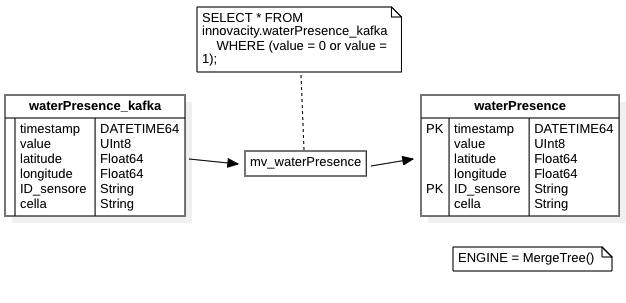
\includegraphics[width=1\textwidth]{../Images/SpecificaTecnica/waterPresence.png}
  \caption{Tabella waterPresence\_kafka e waterPresence}
  \label{fig:waterPresence_tables}
\end{figure}

%_____________________________________________________________________________

\subsubsection{Punteggi di salute}
Viene create anche una tabella dedicata alla persistenza dei punteggi di salute nel tempo calcolati per ogni cella della città. La tabella di destinazione ClickHouse è nominata ‘HealthScores’, i campi sono: cella (String), value (Float32), timestamp(DATETIME64).


\begin{figure}[H]
  \centering
  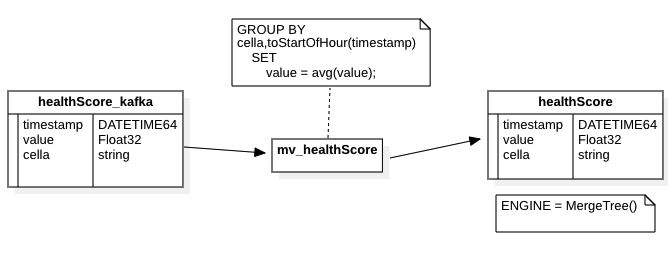
\includegraphics[width=1\textwidth]{../Images/SpecificaTecnica/healthScore.png}
  \caption{Tabella HealthScore\_kafka e HealthScore}
  \label{fig:HealthScore_tables}
\end{figure}

\paragraph(Time to Live)
La tabella dedicata alle misurazioni di salute include la configurazione di un TTL (Time-to-Live) che consente l'aggregazione dei dati dopo un mese dal timestamp della "misurazione" in una singola "misurazione" per cella e per ora. Questo approccio consente di ridurre l'utilizzo dello spazio di archiviazione e accelerare il tempo di interrogazione, mantenendo comunque un livello di dettaglio adeguato per le analisi.







\subsection{Grafana}
Grafana è un software open source per la visualizzazione e l'analisi dei dati. È progettato per funzionare con vari database di serie temporali, tra cui Clickhouse. Grafana offre un'interfaccia utente intuitiva e flessibile che consente di creare e condividere dashboard personalizzate per monitorare i dati in tempo reale. È ampiamente utilizzato per monitorare sistemi e applicazioni, nonché per analizzare e visualizzare dati in tempo reale.

\subsubsection{Utenti}
L'accesso a Grafana è vincolato a due utenze e non permette uteriori registrazioni per l'accesso alla piattaforma di monitoraggio.
\begin{itemize}
    \item \textbf{Amministratore:} 
    \begin{itemize}
        \item Accesso riservato all'amministratore di sistema per permettere manutenzione e modifiche alle impostazioni sensibili della piattaforma.
        \item Non accessibile in produzione.
    \end{itemize}
    
    \item \textbf{User:} 
    \begin{itemize}
        \item Accesso riservato alle autorità locali per la visualizzazione e l'analisi dei dati.
        \begin{itemize}
            \item \textbf{Username:} user
            \item \textbf{Password:} user
        \end{itemize} 
    \end{itemize}
\end{itemize}

\subsubsection{Dashboards}
Per soddisfare tutti i requisiti definiti in \textit{Analisi dei requisiti v2.0.0} sono state create due Dashboard:
\begin{itemize}
    \item \textbf{Dashboard Principale:} Questa dashboard fornisce una visualizzazione chiara e intuitiva delle misurazioni provenienti da tutti i sensori, di tutte le tipologie, distribuiti nell'area urbana. La dashboard include una mappa interattiva della città che mostra la posizione geografica di ciascun sensore e la relativa ultima misurazione. Inoltre, viene presentato il punteggio di salute della città o di celle specifiche.
    \item \textbf{Dashboard dedicata:} Mostra le misurazioni di una specifica tipologia di sensore selezionata dall'utente in modo più dettagliato e permette di effettuare le attività di filtraggio e aggregazione definite in \textit{Analisi dei requisiti v2.0.0}.
\end{itemize}



\paragraph*{Dashboard Principale - Progettazione in dettaglio}
La dashboard principale è suddivisa in righe comprimibili. Di seguito, vengono elencate le informazioni da visualizzare per ciascuna riga, nell’ordine dall'enumerazione, \textbf{ l'intervallo di tempo scelto dall'utente tramite interfaccia di default Grafana verrà chiamato \textit{UserInterval}.}
\begin{enumerate}
    \item Titolo riga: \textbf{City manager}
    \begin{enumerate}
        \item Pannello per la scelta delle celle della città cui si intende visualizzare le misurazioni;
        \item Mappa interattiva della città, presenta i sensori interni alle celle selezionate
        \item Pannello per la visualizzazione del punteggio di salute relativo alla celle selezionate;
        \item Pannello per la visualizzazione dello stato degli alert relativi alle celle selezionate.
    \end{enumerate}
    \item Titolo riga: \textbf{Temperatura}
    \begin{enumerate}
        \item Pannello per la scelta dei sensori di temperatura da analizzare, (vengono proposti per la scelta solo i sensori interni alle celle selezionate per l'analisi);
        \textbf{Verrà chiamato \textit{tmps} l'insieme dei sensori di temperatura scelti nel pannello appena esposto e presenti nelle celle selezionate nel pannello apposito.}
        \item Pannello con vista time-series delle misurazioni di temperatura, vengono presentati le misurazioni dei sensori \textit{tmps} in \textit{UserInterval}
        \item Pannello con vista della media delle misurazioni dei sensori \textit{tmps} in \textit{UserInterval}.
    \end{enumerate}
    \item Titolo riga: \textbf{Umidità}
    \begin{enumerate}
        \item Pannello per la scelta dei sensori di umidità da analizzare, (vengono proposti per la scelta solo i sensori interni alle celle selezionate per l'analisi);
        \textbf{Verrà chiamato \textit{umids} l'insieme dei sensori di umidità scelti nel pannello appena esposto e presenti nelle celle selezionate nel pannello apposito.}
        \item Pannello con vista time-series delle misurazioni di umidità, vengono presentati le misurazioni dei sensori \textit{umids} in \textit{UserInterval}
        \item Pannello con vista della media delle misurazioni dei sensori \textit{umids} in \textit{UserInterval}.
    \end{enumerate}
    \item Titolo riga: \textbf{Polveri sottili}
    \begin{enumerate}
        \item Pannello per la scelta dei sensori di polveri sottili da analizzare, (vengono proposti per la scelta solo i sensori interni alle celle selezionate per l'analisi);
        \textbf{Verrà chiamato \textit{pm\_sensors} l'insieme dei sensori di polveri sottili scelti nel pannello appena esposto e presenti nelle celle selezionate nel pannello apposito.}
        \item Pannello con vista time-series delle misurazioni di polveri sottili, vengono presentati le misurazioni dei sensori \textit{pm\_sensors} in \textit{UserInterval};
        \item Pannello con vista della media delle misurazioni dei sensori \textit{pm\_sensors} in \textit{UserInterval}.
    \end{enumerate}
    \item Titolo riga: \textbf{Isole ecologiche}
    \begin{enumerate}
        \item Pannello per la scelta delle isole ecologiche da analizzare, (vengono proposte per la scelta solo le isole ecologiche interne alle celle selezionate per l'analisi);
        \textbf{Verrà chiamato \textit{islands} l'insieme delle isole ecologiche scelte nel pannello appena esposto.}
        \item Pannello con vista time-series delle misurazioni delle isole ecologiche, vengono presentate le misurazioni delle isole ecologiche \textit{islands} in \textit{UserInterval}
        \item Pannello con vista della media delle misurazioni delle isole ecologiche \textit{islands} in \textit{UserInterval}.
    \end{enumerate}
\item Titolo riga: \textbf{Colonnine di ricarica}
\begin{enumerate}
    \item Pannello per la scelta delle colonnine di ricarica da analizzare, (vengono proposte per la scelta solo le  colonnine di ricarica interne alle celle selezionate per l'analisi);
    \textbf{Verrà chiamato \textit{chsSt} l'insieme delle  colonnine di ricarica scelte nel pannello appena esposto.}
    \item Pannello con vista sul numero di colonnine di ricarica libere in \textit{chsSt} considerato l'ultima misurazione in
    \textit{UserInterval} 
    \item Pannello con vista sul numero di colonnine di ricarica occupate in \textit{chsSt} considerato l'ultima misurazione in \textit{UserInterval} 
    \item Pannello con vista tabellare delle ultime misurazioni in \textit{UserInterval} delle colonnine di ricarica in \textit{chsSt}.
\end{enumerate}
\item Titolo riga: \textbf{Guasti elettrici}
\begin{enumerate}
    \item Pannello per la scelta dei sensori di guasti elettrici da analizzare, (vengono proposti per la scelta solo i sensori di guasti elettrici interni alle celle selezionate per l'analisi);
    \textbf{Verrà chiamato \textit{GstEl} l'insieme dei sensori di guasti elettrici scelti nel pannello appena esposto.}
    \item Pannello con vista sul numero di sensori che hanno rilevato anomalie in \textit{GstEl} considerato l'ultima misurazione in \textit{UserInterval} 
    \item Pannello con vista sul numero di sensori che non  hanno rilevato anomalie in \textit{GstEl} considerato l'ultima misurazione in \textit{UserInterval} 
    \item Pannello con vista tabellare delle ultime misurazioni in \textit{UserInterval} dei sensori \textit{GstEl}.
\end{enumerate}
\item Titolo riga: \textbf{Sensori di presenza dell'acqua}
\begin{enumerate}
\item Pannello per la selezione dei sensori di presenza dell'acqua da analizzare (vengono proposti solo i sensori di presenza dell'acqua interni alle celle selezionate per l'analisi);
\textbf{Verrà chiamato \textit{PresAcq} l'insieme dei sensori di presenza dell'acqua scelti nel pannello appena esposto.}
\item Pannello con vista sul numero di sensori che hanno rilevato acqua in \textit{PresAcq} considerando l'ultima misurazione nell'intervallo temporale definito dall'utente (\textit{UserInterval}).
\item Pannello con vista sul numero di sensori che non hanno rilevato acqua in \textit{PresAcq} considerando l'ultima misurazione nell'intervallo temporale definito dall'utente (\textit{UserInterval}).
\item Pannello con vista tabellare delle ultime misurazioni nell'intervallo (\textit{UserInterval}) dei sensori \textit{PresAcq}.
\end{enumerate}
\end{enumerate}


\paragraph*{Dashboard dedicata - Progettazione in dettaglio}
La dashboard dedicata è suddivisa in due sezioni: la prima posta nella parte superiore della dashboard è dedicata ai pannelli per le variabili di input, mentre la seconda posta nella parte inferiore della dashboard è dedicata alla visualizzazione delle misurazioni dei sensori secondo le impostazioni selezionate.\\
Di seguito vengono esposti i dettagli relativi alla progettazione della selezione delle variabili di input:
\begin{enumerate}
    \item Nome pannello: \textbf{Selezione cella}: Permette di selezionare le celle della città da analizzare;
    \item Nome pannello: \textbf{Tipologia misurazioni}: Permette di selezionare la tipologia di sensori da analizzare;
    \item Nome pannello variabili: \textbf{Seleziona i sensori}: Permette di selezionare i sensori da analizzare della tipologia e della cella selezionata;
    \item Nome pannello: \textbf{Aggregazione temporale}: Permette di selezionare l'intervallo temporale di aggregazione delle misurazioni:{Automatico, Secondo, Minuto, Ora, Giorno, Mese, Nessuno}. Maggiori dettagli in \ref{sec:var_dedicate};
    \item Nome pannello: \textbf{Misurazine minima}: Permette di selezionare il valore minimo delle misurazioni da visualizzare;
    \item Nome pannello: \textbf{Misurazione massima}: Permette di selezionare il valore massimo delle misurazioni da visualizzare.
\end{enumerate}
Di seguito vengono esposti i dettagli relativi alla progettazione della visualizzazione delle misurazioni secondo le variabili selezionate:
\begin{enumerate}
    \item Nome pannello: \textbf{Grafico a linee}: Visualizzazione delle misurazioni avviene attraverso un grafico a linee time-series. Le misurazioni sono mostrate in base ai parametri specificati dall’utente. In particolare, le misurazioni esposte si basano sulla selezione delle celle, dei sensori, della tipologia delle misurazioni, dell’aggregazione temporale e della misurazione massima e minima definita dall’utente;
    \item Nome pannello: \textbf{Tabella misurazioni}: Visualizzazione delle misurazioni in forma tabellare. Come nel pannello precedente, le misurazioni sono mostrate in base ai parametri specificati dall'utente.
\end{enumerate}

\subsubsection{ClickHouse data source plugin} \label{sec:click_plugin}
\paragraph{Documentazione:}
\href{https://grafana.com/grafana/plugins/grafana-clickhouse-datasource/}{https://grafana.com/grafana/plugins/grafana-clickhouse-datasource/}

Questo plugin di grafana consente di connettersi a un'istanza di ClickHouse e di visualizzare i dati in tempo reale. È possibile eseguire query SQL personalizzate e visualizzare i risultati in forma di grafici, tabelle e pannelli personalizzati. Il plugin offre anche funzionalità di aggregazione e di calcolo dei dati, consentendo di analizzare e visualizzare i dati in modo flessibile e personalizzato.

\paragraph{Data sources configuration}
La configurazione del data source avviene tramite file \textit{yaml} che deve essere presente in \textit{"grafana/provisioning/datasources"}.
Il protocollo di trasporto utilizzato è TLS ma puo essere modificato nel file appena citato grazie al parametro di configurazione: "protocol".

\paragraph{Macro utilizzate}\label{sec:macros}
Per semplificare la sintassi e consentire operazioni dinamiche, come i filtri dell'intervallo di date, le queries al database Clickhouse possono contenere macro.
Quelle utilizzate sono:
\begin{itemize}
    \item \textbf{\$\_\_timeFilter(columnName)}: Permette di effettuare il filtro temporale alla query per ottenere le sole misurazioni all'interno dell'intervallo di tempo selezionato dall'utente.
    \item  \textbf{\$\_\_timeInterval(columnName)}: Permette di modificare il raggruppamento temporale delle misurazioni in automatico sulla base dell'ampiezza dell'intervallo temporale selezionato dall'utente.
    In questo modo è possibile avere una visione ottimizzate delle misurazioni.
\end{itemize}

\subsubsection{Variabili Grafana}
\paragraph*{Documentazione:}
 \href{https://grafana.com/docs/grafana/latest/dashboards/variables/}{https://grafana.com/docs/grafana/latest/dashboards/variables/}


 Le variabili in Grafana sono un potente strumento per rendere le dashboard dinamiche e interattive. Permettono di filtrare i dati visualizzati in base a valori scelti dall'utente, rendendo la dashboard più versatile e adattabile a differenti esigenze.
\paragraph*{Utilizzo delle variabili nella dashboard principale:}
Nella dashboard principale, le variabili sono:
\begin{itemize}
    \item \textbf{variabile (\$cella)}: per mostrare solo le misurazioni provenienti da determinate celle della città, 
    \item \textbf{variabili (\$<TipoSensore>\_sensors\_id)}: per mostrare le misurazioni di determinati sensori di un certo tipo.
\end{itemize}
Queste variabili all'interno delle query al database permettono il filtraggio delle misurazioni sulla base di quanto selezionato dall'utente.
Un esempio di query per la visualizzazione delle misurazioni time-series di temperatura è:
\begin{lstlisting}[style=code]
    SELECT    ID_sensore, avg(value) as value,
              $__timeInterval(timestamp) as timestamp
    FROM    innovacity.temperatures 
    WHERE    $__timeFilter(timestamp) AND cella IN ($Cella) AND ID_sensore in (${tmp_sensors_id})
    GROUP BY ID_sensore, timestamp;
\end{lstlisting}

La query esposta mostra anche l'utilizzo delle macro esposte in: \ref{sec:macros}
\paragraph*{Utilizzo delle variabili nella dashboard dedicata:} \label{sec:var_dedicate}
Nella dashboard dedicata alla visualizzazione spefica delle misurazioni di una sola tipologia di sensori, le variabili sono:
\begin{itemize}
    \item \textbf{variabile (\$cella)}: per mostrare solo le misurazioni provenienti da determinate celle della città, 
    \item \textbf{variabili (\$<TipoSensore>\_sensors\_id)}: per mostrare le misurazioni di determinati sensori di un certo tipo.
    \item \textbf{variabili (\$tabella)}: per selezionare la tipoligia di sensore di cui si vuole visualizzare la dashboard dedicata e quindi la tabella del database da cui ricavare i dati.
    \item \textbf{(\$aggregazione)}: variabile per selezionare l'intervallo temporale di aggregazione delle misurazioni
    (Automatico, Secondo,Minuto,Ora,Giorno,Mese,Nessuno).
    Nel caso della selezione della modalità "Automatico" si utilizzza l'intervallo temporale di aggregazione più opportuno sulla base dell'ampiezza dell'intervallo temporale selezionato dall'utente.
    \item \textbf{(\$Max\_value)}: variabile ad input numerico per filtrare le misurazioni con valore al di sotto di quello indicato.
    \item \textbf{(\$Min\_value)}: variabile ad input numerico per filtrare le misurazioni con valore al di sopra di quello indicato.
\end{itemize}
\paragraph{Variable Panel plugin}
\textbf{Documentazione:}
\href{https://volkovlabs.io/plugins/volkovlabs-variable-panel/}{https://volkovlabs.io/plugins/volkovlabs-variable-panel/}


Il plugin permette di creare dei pannelli grafana che possono essere posizionati ovunque nella Dashboard e che consentono di selezionare i valori delle variabili.
Inoltre permette la visualizzazione ad albero delle variabili utile nel nostro caso dove i sensori sono contenuti all'interno di celle della città.

\subsubsection{Grafana alerts}
\textbf{Documentazione}

\href{https://grafana.com/docs/grafana/latest/alerting/}{https://grafana.com/docs/grafana/latest/alerting/}


Grafana offre un sistema di alerting completo per monitorare i dati e inviare notifiche quando si verificano determinate condizioni. Le notifiche possono essere inviate tramite diversi canali, tra cui email, Slack, Telegram e Discord.

\paragraph{Alert Rule}
Per poter configurare un alert è necessario creare una regola di alert. La regola di alert viene impostata tramite query al data source e fa scattare l'alert quando la query restituisce un risultato che soddisfa le condizioni impostate.
Gli alert impostati sono per:
\begin{itemize}
    \item Quando un sensore di temperatura registra una temperatura superiore ai 40°C o inferiore ai -10°C;
    \item Quando un sensore di polveri sottili supera i 50 microgrammi al metro cubo;
    \item Quando un sensore di guasti elettrici rileva un guasto.
\end{itemize}

Gli alert attraversano 3 stati:
\begin{itemize}
    \item \textbf{Pending:} indica che un alert è stato attivato, ma la sua valutazione non è ancora stata completata.
                            Quando si è in questo stato è perchè il valore della query di alert è stato valutato e risulta essere vero ma la configurazione della regola di allerta ha impostato che l'allerta deve essere attiva per un certo periodo di tempo prima di essere considerata vera e quindi inviare la notifica.
\item \textbf{Firing:}  indica che un alert è stato attivato e la sua valutazione ha confermato che la condizione di alert è soddisfatta per il periodo impostato nella regola e quindi viene inviata la notifica ai canali impostati.
\item \textbf{OK:} indica che un alert è stato disattivato e la sua valutazione ha confermato che la condizione di alert non è più soddisfatta.

Le regole di allerta sono impostabili tramite l'interfaccia grafica di Grafana e vengono esportate in formato \textit{yaml} ed inserite in "/provisioning/alerting".
                            
\end{itemize}

\paragraph{Configurazione il canale di notifica}
Per configurare i canali di notifica è necessario andare in "Alerting" e selezionare "Notification channels" dall'interfaccia grafica di Grafana.

Per il progetto è stato scelto Discord come unico canale di notifica.
Per configurare il canale di notifica è necessario:
\begin{itemize}
    \item Seleziona Discord come canale di notifica.
    \item Configurazione Server Discord "Innovacity":
    \begin{itemize}
        \item Il server discord è stato creato ed è raggiungibile tramite l'indirizzo: \href{https://discord.gg/cCp9qxK7}{https://discord.gg/cCp9qxK7}
        \item Per ottenerre il webhook URL del canale Discord andare in : \textit{Impostazioni server/Integrazioni} e seleziona "visualizza webhook".
    \end{itemize}
    \item Inserisci il webhook URL del tuo canale Discord.
    \item Personalizza il messaggio di notifica.
    
\end{itemize}

Anche le impostazioni di configurazione del canale di notifica sono esportabili in formato \textit{yaml} e vengono inserite in "/provisioning/alerting".



\paragraph{Notification policies}
Le norme di notifica negli Alert di Grafana sono un modo potente per gestire l'invio degli alert a diversi canali di notifica.

Per una spiegazione dettagliata della configurazione si rimanda alla documentazione ufficiale di Grafana: \href{https://grafana.com/docs/grafana/latest/alerting/alerting-rules/create-notification-policy/}{https://grafana.com/docs/grafana/latest/alerting/alerting-rules/create-notification-policy/}

Anche le impostazioni delle notification policies sono esportabili in formato \textit{yaml} e vengono inserite in "/provisioning/alerting".

\subsubsection{Altri plugin utilizzati}
\paragraph{Orchestra Cities Map plugin}
\textbf{Documentazione:}

\href{https://grafana.com/grafana/plugins/orchestracities-map-panel/}{https://grafana.com/grafana/plugins/orchestracities-map-panel/}

Il plugin Orchestra Cities Map per Grafana estende il pannello Geomap di Grafana con diverse funzionalità avanzate per la visualizzazione di dati geolocalizzati su mappe:

Funzionalità principali:
\begin{itemize}
    \item \textbf{Supporto per GeoJSON}: Permette di visualizzare dati geoJSON su mappe, come shapefile di città, regioni o stati.
    \item \textbf{Icone personalizzate}: Puoi utilizzare icone personalizzate per rappresentare diversi tipi di dati sui punti mappa.
    \item \textbf{Popup informativi}: Mostra popup con informazioni dettagliate quando si clicca su un punto mappa.
    \item \textbf{Strati multipli}: Permette di creare più strati sovrapposti per visualizzare diversi set di dati sulla stessa mappa.
    \item \textbf{Filtraggio e ricerca}: Puoi filtrare i punti mappa in base a diversi criteri, come proprietà dei dati o valori delle metriche.
    \item \textbf{Colorazione dei punti}: Puoi colorare i punti mappa in base a valori di metriche o ad altri criteri.
    \item \textbf{Legende personalizzate}: Puoi creare legende personalizzate per spiegare il significato dei colori e delle icone utilizzati nella mappa.
\end{itemize}

Viene utilizzato per poter visualizzare in modo diverse le icone dei diversi tipi di sensori dislocati nella città oltre che l'ultima misurazione effettuata ovvero lo stato attuale del sensore.
